% Options for packages loaded elsewhere
\PassOptionsToPackage{unicode}{hyperref}
\PassOptionsToPackage{hyphens}{url}
%
\documentclass[
]{book}
\usepackage{amsmath,amssymb}
\usepackage{iftex}
\ifPDFTeX
  \usepackage[T1]{fontenc}
  \usepackage[utf8]{inputenc}
  \usepackage{textcomp} % provide euro and other symbols
\else % if luatex or xetex
  \usepackage{unicode-math} % this also loads fontspec
  \defaultfontfeatures{Scale=MatchLowercase}
  \defaultfontfeatures[\rmfamily]{Ligatures=TeX,Scale=1}
\fi
\usepackage{lmodern}
\ifPDFTeX\else
  % xetex/luatex font selection
\fi
% Use upquote if available, for straight quotes in verbatim environments
\IfFileExists{upquote.sty}{\usepackage{upquote}}{}
\IfFileExists{microtype.sty}{% use microtype if available
  \usepackage[]{microtype}
  \UseMicrotypeSet[protrusion]{basicmath} % disable protrusion for tt fonts
}{}
\makeatletter
\@ifundefined{KOMAClassName}{% if non-KOMA class
  \IfFileExists{parskip.sty}{%
    \usepackage{parskip}
  }{% else
    \setlength{\parindent}{0pt}
    \setlength{\parskip}{6pt plus 2pt minus 1pt}}
}{% if KOMA class
  \KOMAoptions{parskip=half}}
\makeatother
\usepackage{xcolor}
\usepackage{color}
\usepackage{fancyvrb}
\newcommand{\VerbBar}{|}
\newcommand{\VERB}{\Verb[commandchars=\\\{\}]}
\DefineVerbatimEnvironment{Highlighting}{Verbatim}{commandchars=\\\{\}}
% Add ',fontsize=\small' for more characters per line
\usepackage{framed}
\definecolor{shadecolor}{RGB}{248,248,248}
\newenvironment{Shaded}{\begin{snugshade}}{\end{snugshade}}
\newcommand{\AlertTok}[1]{\textcolor[rgb]{0.94,0.16,0.16}{#1}}
\newcommand{\AnnotationTok}[1]{\textcolor[rgb]{0.56,0.35,0.01}{\textbf{\textit{#1}}}}
\newcommand{\AttributeTok}[1]{\textcolor[rgb]{0.13,0.29,0.53}{#1}}
\newcommand{\BaseNTok}[1]{\textcolor[rgb]{0.00,0.00,0.81}{#1}}
\newcommand{\BuiltInTok}[1]{#1}
\newcommand{\CharTok}[1]{\textcolor[rgb]{0.31,0.60,0.02}{#1}}
\newcommand{\CommentTok}[1]{\textcolor[rgb]{0.56,0.35,0.01}{\textit{#1}}}
\newcommand{\CommentVarTok}[1]{\textcolor[rgb]{0.56,0.35,0.01}{\textbf{\textit{#1}}}}
\newcommand{\ConstantTok}[1]{\textcolor[rgb]{0.56,0.35,0.01}{#1}}
\newcommand{\ControlFlowTok}[1]{\textcolor[rgb]{0.13,0.29,0.53}{\textbf{#1}}}
\newcommand{\DataTypeTok}[1]{\textcolor[rgb]{0.13,0.29,0.53}{#1}}
\newcommand{\DecValTok}[1]{\textcolor[rgb]{0.00,0.00,0.81}{#1}}
\newcommand{\DocumentationTok}[1]{\textcolor[rgb]{0.56,0.35,0.01}{\textbf{\textit{#1}}}}
\newcommand{\ErrorTok}[1]{\textcolor[rgb]{0.64,0.00,0.00}{\textbf{#1}}}
\newcommand{\ExtensionTok}[1]{#1}
\newcommand{\FloatTok}[1]{\textcolor[rgb]{0.00,0.00,0.81}{#1}}
\newcommand{\FunctionTok}[1]{\textcolor[rgb]{0.13,0.29,0.53}{\textbf{#1}}}
\newcommand{\ImportTok}[1]{#1}
\newcommand{\InformationTok}[1]{\textcolor[rgb]{0.56,0.35,0.01}{\textbf{\textit{#1}}}}
\newcommand{\KeywordTok}[1]{\textcolor[rgb]{0.13,0.29,0.53}{\textbf{#1}}}
\newcommand{\NormalTok}[1]{#1}
\newcommand{\OperatorTok}[1]{\textcolor[rgb]{0.81,0.36,0.00}{\textbf{#1}}}
\newcommand{\OtherTok}[1]{\textcolor[rgb]{0.56,0.35,0.01}{#1}}
\newcommand{\PreprocessorTok}[1]{\textcolor[rgb]{0.56,0.35,0.01}{\textit{#1}}}
\newcommand{\RegionMarkerTok}[1]{#1}
\newcommand{\SpecialCharTok}[1]{\textcolor[rgb]{0.81,0.36,0.00}{\textbf{#1}}}
\newcommand{\SpecialStringTok}[1]{\textcolor[rgb]{0.31,0.60,0.02}{#1}}
\newcommand{\StringTok}[1]{\textcolor[rgb]{0.31,0.60,0.02}{#1}}
\newcommand{\VariableTok}[1]{\textcolor[rgb]{0.00,0.00,0.00}{#1}}
\newcommand{\VerbatimStringTok}[1]{\textcolor[rgb]{0.31,0.60,0.02}{#1}}
\newcommand{\WarningTok}[1]{\textcolor[rgb]{0.56,0.35,0.01}{\textbf{\textit{#1}}}}
\usepackage{longtable,booktabs,array}
\usepackage{calc} % for calculating minipage widths
% Correct order of tables after \paragraph or \subparagraph
\usepackage{etoolbox}
\makeatletter
\patchcmd\longtable{\par}{\if@noskipsec\mbox{}\fi\par}{}{}
\makeatother
% Allow footnotes in longtable head/foot
\IfFileExists{footnotehyper.sty}{\usepackage{footnotehyper}}{\usepackage{footnote}}
\makesavenoteenv{longtable}
\usepackage{graphicx}
\makeatletter
\def\maxwidth{\ifdim\Gin@nat@width>\linewidth\linewidth\else\Gin@nat@width\fi}
\def\maxheight{\ifdim\Gin@nat@height>\textheight\textheight\else\Gin@nat@height\fi}
\makeatother
% Scale images if necessary, so that they will not overflow the page
% margins by default, and it is still possible to overwrite the defaults
% using explicit options in \includegraphics[width, height, ...]{}
\setkeys{Gin}{width=\maxwidth,height=\maxheight,keepaspectratio}
% Set default figure placement to htbp
\makeatletter
\def\fps@figure{htbp}
\makeatother
\ifLuaTeX
  \usepackage{luacolor}
  \usepackage[soul]{lua-ul}
\else
  \usepackage{soul}
\fi
\setlength{\emergencystretch}{3em} % prevent overfull lines
\providecommand{\tightlist}{%
  \setlength{\itemsep}{0pt}\setlength{\parskip}{0pt}}
\setcounter{secnumdepth}{5}
\usepackage{booktabs}
\ifLuaTeX
  \usepackage{selnolig}  % disable illegal ligatures
\fi
\usepackage[]{natbib}
\bibliographystyle{plainnat}
\usepackage{bookmark}
\IfFileExists{xurl.sty}{\usepackage{xurl}}{} % add URL line breaks if available
\urlstyle{same}
\hypersetup{
  pdftitle={ADS - Engenharia de Software 2025 - Anotações de aula},
  pdfauthor={Professor Miguel Suez Xve Penteado},
  hidelinks,
  pdfcreator={LaTeX via pandoc}}

\title{ADS - Engenharia de Software 2025 - Anotações de aula}
\author{Professor Miguel Suez Xve Penteado}
\date{2025-03-25}

\begin{document}
\maketitle

{
\setcounter{tocdepth}{1}
\tableofcontents
}
\chapter*{Sobre estas anotações}\label{sobre-estas-anotauxe7uxf5es}
\addcontentsline{toc}{chapter}{Sobre estas anotações}

Estas anotações são apenas lembretes das aulas expostas em sala, durante a disciplina de ENGENHARIA DE SOFTWARE.

\subsection{ACESSO AO GITBOOK CELULAR}\label{acesso-ao-gitbook-celular}

\subsection{\texorpdfstring{\url{https://miguel7penteado.github.io/ADS-EngenhariaSoftware2025}}{https://miguel7penteado.github.io/ADS-EngenhariaSoftware2025}}\label{httpsmiguel7penteado.github.ioads-engenhariasoftware2025}


\includegraphics{images/qr-code-disciplina.jpg}

\subsection{APP EPUB ANDROID}\label{app-epub-android}

\subsection{\texorpdfstring{\textbf{Moon+ Reader}}{Moon+ Reader}}\label{moon-reader}


\includegraphics{images/qrcode/leitor_epub/MoonReaderPlus.jpg}

\subsection{Livros Texto da Disciplina}\label{livros-texto-da-disciplina}

\subsubsection{``Engenharia de Software'' do autor ``Roger S Pressman''}\label{engenharia-de-software-do-autor-roger-s-pressman}

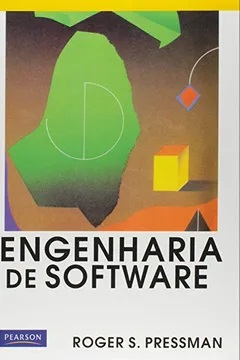
\includegraphics{images/livros/engenharia_software_pressman.jpg}

\begin{longtable}[]{@{}
  >{\raggedright\arraybackslash}p{(\columnwidth - 2\tabcolsep) * \real{0.5000}}
  >{\raggedright\arraybackslash}p{(\columnwidth - 2\tabcolsep) * \real{0.5000}}@{}}
\toprule\noalign{}
\endhead
\bottomrule\noalign{}
\endlastfoot
\textbf{Autor(es)} & \href{https://www.indicalivros.com/autores?q=Roger\%20S.\%20Pressman}{Roger S. Pressman} \\
\textbf{Editora} & Pearson \\
\textbf{Idioma} & Português \\
\textbf{ISBN} & 8534602379 9788534602372 \\
\textbf{Formato} & Capa comum \\
\textbf{Páginas} & 1056 \\
\textbf{Código Biblioteca} & \\
\end{longtable}

\subsubsection{``Engenharia de Software'' do autor ``Ian Sommerville''}\label{engenharia-de-software-do-autor-ian-sommerville}

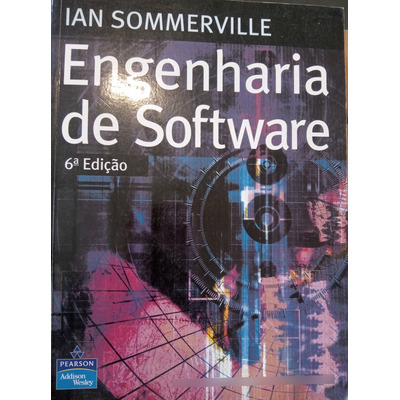
\includegraphics{images/livros/engenharia_software_sommerville.jpg}

\begin{longtable}[]{@{}ll@{}}
\toprule\noalign{}
\endhead
\bottomrule\noalign{}
\endlastfoot
\textbf{Autor(es)} & Ian SommerVille \\
\textbf{Editora} & Pearson \\
\textbf{Idioma} & Português \\
\textbf{ISBN} & 9788588639072 \\
\textbf{Formato} & Capa comum \\
\textbf{Páginas} & 768 \\
\textbf{Código Biblioteca} & \\
\end{longtable}

Calendário das aulas

\paragraph{FEVEREIRO 2025}\label{fevereiro-2025}

\begin{longtable}[]{@{}lll@{}}
\toprule\noalign{}
\endhead
\bottomrule\noalign{}
\endlastfoot
Data & Dia da semana & Aulas \\
4 de fevereiro & Terça-feira & Recesso \\
11 de fevereiro & Terça-feira & Recesso \\
18 de fevereiro & Terça-feira & Aula Inaugural \\
25 de fevereiro & Terça-feira & Qualidade de Software I \\
\end{longtable}

\paragraph{MARÇO 2025}\label{maruxe7o-2025}

\begin{longtable}[]{@{}lll@{}}
\toprule\noalign{}
\endhead
\bottomrule\noalign{}
\endlastfoot
Data & Dia da semana & Aulas \\
4 de março & Terça-feira & Carnaval \\
11 de março & Terça-feira & Verificação e Validação de Software I \\
18 de março & Terça-feira & Verificação e Validação de Software II \\
25 de março & Terça-feira & \\
\end{longtable}

\paragraph{ABRIL DE 2025}\label{abril-de-2025}

\begin{longtable}[]{@{}lll@{}}
\toprule\noalign{}
\endhead
\bottomrule\noalign{}
\endlastfoot
Data & Dia da semana & Aulas \\
1 de abril & Terça-feira & Prova NP1 \\
8 de abril & Terça-feira & Manutenção de software I \\
15 de abril & Terça-feira & Manutenção de software II \\
22 de abril & Terça-feira & Manutenção de software III \\
29 de abril & Terça-feira & Manutenção de software IV \\
\end{longtable}

\paragraph{MAIO DE 2025}\label{maio-de-2025}

\begin{longtable}[]{@{}lll@{}}
\toprule\noalign{}
\endhead
\bottomrule\noalign{}
\endlastfoot
Data & Dia da semana & Aulas \\
6 de maio & Terça-feira & Gerência de Configuração \\
13 de maio & Terça-feira & Revisão \\
20 de maio & Terça-feira & Prova NP2 \\
27 de maio & Terça-feira & Substitutiva \\
\end{longtable}

\paragraph{JUNHO DE 2025}\label{junho-de-2025}

\begin{longtable}[]{@{}lll@{}}
\toprule\noalign{}
\endhead
\bottomrule\noalign{}
\endlastfoot
Data & Dia da semana & Aulas \\
3 de junho & Terça-feira & Plantão \\
10 de junho & Terça-feira & Plantão \\
17 de junho & Terça-feira & Exame \\
24 de junho & Terça-feira & \\
\end{longtable}

\subsection{Alunos 2025}\label{alunos-2025}

\subsubsection{Turma DS2P40}\label{turma-ds2p40}

\begin{longtable}[]{@{}ll@{}}
\toprule\noalign{}
Matrícula & Nome do Aluno \\
\midrule\noalign{}
\endhead
\bottomrule\noalign{}
\endlastfoot
F35HFJ-1 & BEATRIZ ALMEIDA DA SILVA \\
R54885-6 & BRENO SOUZA MASCARENHAS \\
R19267-9 & CARLOS EDUARDO DA S GALDINO \\
R150FH-8 & DANILO LUCAS LOURENCO \\
G740IF-9 & GUSTAVO ALCANTARA NOBRE \\
G76IBD-7 & HELLEN REGINA B DOS SANTOS \\
F35EBD-4 & JOAO ALFREDO DA S BRENNER \\
R11835-5 & LUCAS ROSSE \\
G839GC-6 & PABLO HENRIQUE C ARAUJO \\
G61ICI-3 & THIAGO VERNIER LOUREIRO MAIA \\
\end{longtable}

\subsubsection{Turma DS3P40}\label{turma-ds3p40}

\begin{longtable}[]{@{}ll@{}}
\toprule\noalign{}
Matrícula & Nome do Aluno \\
\midrule\noalign{}
\endhead
\bottomrule\noalign{}
\endlastfoot
T736DG-3 & ANDRE LUIS RIGUEIRA ZANA \\
R06534-0 & BIANCA CAVALCANTE DOS SANTOS \\
G964AA-5 & CIBELE MARIA BARBOSA \\
R1007A-0 & DANIEL GOES CARVALHO SILVA \\
G98399-8 & DAVI PEREIRA DO VALE \\
F3567F-6 & EDUARDO MONTINO LACERDA \\
F35973-5 & FELIPE DE CAMPOS MOREIRA ALVES \\
R0622A-5 & FERNANDA VICTORIA D LO VACCO \\
R091EC-3 & GABRIEL ALVES BATISTA \\
G989DC-6 & GABRIEL PINHEIRO SOUZA \\
R08565-1 & GIOVANNY GOMES BRANDAO \\
R055AF-2 & GUILHERME NASCIMENTO R BARBOSA \\
N088EG-0 & GUILHERME R DE OLIVEIRA \\
R06229-5 & GUSTAVO SILVA DOS SANTOS \\
R07095-6 & HENRIQUE MOREIRA BOTELLA \\
R0823C-0 & HENRIQUE P DOS S FRANCISCO \\
G98BGB-2 & IGOR XAVIER DE MATTOS \\
G90JDE-2 & JOAO RICARDO DA SILVA JUNIOR \\
F3590G-2 & JOAO RICK GALDINO PEREIRA \\
R0567D-6 & JOAO VICTOR CARVALHO DE SOUZA \\
G9756E-6 & JOAO VICTOR DA SILVA MACHADO \\
G0249I-6 & JULIANA BORGES MOURA \\
F35937-9 & MATHEUS SERVULO CAJE \\
R10099-5 & MELISSA SCARPINATTI B DA SILVA \\
G8832G-1 & RENAN PRAZERES CLEMENTINO \\
F35CDF-2 & SERGIO ALEXANDRE A DO AMARAL \\
\end{longtable}

\subsubsection{Turma DS3Q40}\label{turma-ds3q40}

Com base nas informações da fonte \textbf{``DS3Q40.pdf''} e em nossa conversa anterior, apresento novamente a tabela com a coluna \textbf{Matrícula} (RA) e \textbf{Nome do Aluno} da turma \textbf{DS3Q40}:

\begin{longtable}[]{@{}ll@{}}
\toprule\noalign{}
Matrícula & Nome do Aluno \\
\midrule\noalign{}
\endhead
\bottomrule\noalign{}
\endlastfoot
G003II-9 & ALEX LIMA SILVA \\
G0327I-4 & AMANDA SIMONETTO DIAS \\
G02JDI-5 & ATILA WILLIAM F DE BARROS \\
R096DH-9 & BRENDA RUOTTI \\
R0087I-2 & GUSTAVO SILVA DE ARAUJO \\
G99JAH-4 & JESSICA SANTOS ANJOS \\
G8811G-1 & KAIKY ALVES MONTEIRO \\
G99319-5 & KLEBER WENDEL DE ALMEIDA RIBAS \\
G90EJA-1 & LEONARDO OLIVEIRA DOS SANTOS \\
G99ACJ-8 & LUCAS SILVA PINTO DE ASSIS \\
G99843-0 & MATHEUS ALVES LIMA \\
G996FJ-4 & MATHEUS DE OLIVEIRA MONTEIRO \\
G99JFJ-7 & MATHEUS RIBEIRO DE CAMPOS \\
G9931A-5 & PEDRO HENRIQUE CAMPOS LEAL \\
G012IF-3 & PEDRO PAULO VITALINO \\
R094GC-7 & RENAN DOS SANTOS FERREIRA \\
G96JFG-6 & RICHARD TRISTAN P GARCIA \\
G92GHH-8 & RODRIGO SANTOS ARAUJO \\
G977HG-0 & SIDNEI SERRAO DA SILVA \\
G003IC-0 & THIAGO DA SILVA SEIXEIRO \\
G99566-0 & YASMIN HELENA DE OLIVEIRA FERN \\
\end{longtable}

\chapter*{INTRODUÇÃO A DISCIPLINA DE ENGENHARIA DE SOFTWARE}\label{introduuxe7uxe3o-a-disciplina-de-engenharia-de-software}
\addcontentsline{toc}{chapter}{INTRODUÇÃO A DISCIPLINA DE ENGENHARIA DE SOFTWARE}

Do que trata esta disciplina e o que quer dizer o termo que dá nome a ela ?

\section{O que é ENGENHARIA DE SOFTWARE}\label{o-que-uxe9-engenharia-de-software}

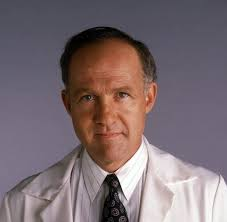
\includegraphics[width=0.95833in,height=\textheight]{images/pressman.jpg}

\begin{quote}
\textbf{Engenharia de Software}~\emph{é o processo de desenvolvimento de programas de computador, estruturas de dados e documentos.} (\textbf{\emph{Roger S. Pressman}})
\end{quote}

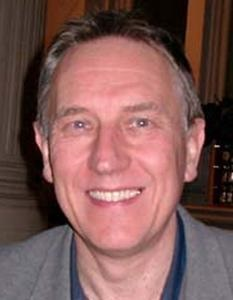
\includegraphics[width=1.0625in,height=\textheight]{images/sommerville.jpg}

\begin{quote}
\textbf{Engenharia de Software} \emph{é uma disciplina de engenharia que se preocupa com todo o processo de produção de software. Isso inclui desde a especificação do sistema até a sua manutenção.} (\textbf{Ian Sommerville})
\end{quote}

É atribuído a \textbf{Margaret Hamilton,} desenvolvedora do programa de navegação da APOLLO 11 a criação do termo ENGENHARIA DE SOFTWARE.

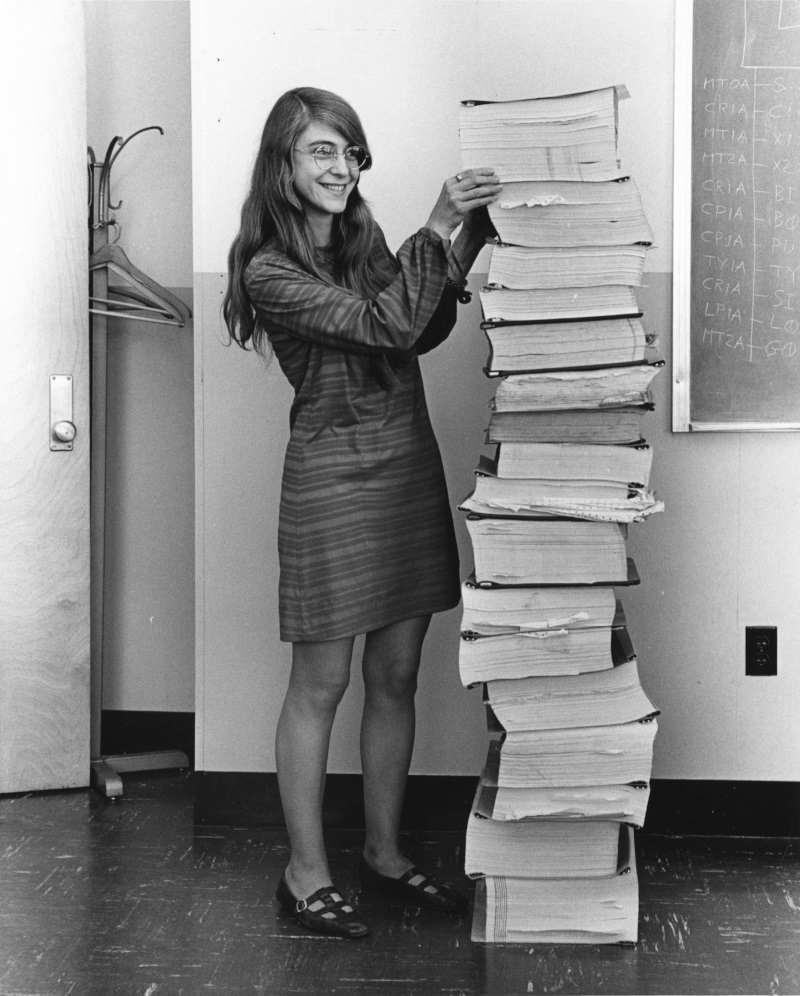
\includegraphics[width=0.5\textwidth,height=\textheight]{images/Margaret_Hamilton.jpg}

\chapter{QUALIDADE DE SOFTWARE}\label{qualidade-de-software}

\section{COMPLIANCE}\label{compliance}

Para que uma organização consiga fechar contrados de venda ou fornecimento com outra organização, especialmente quando o valor do contrato de venda ou prestação é muito alto, há um processo de checagem de COMPLIANCE:

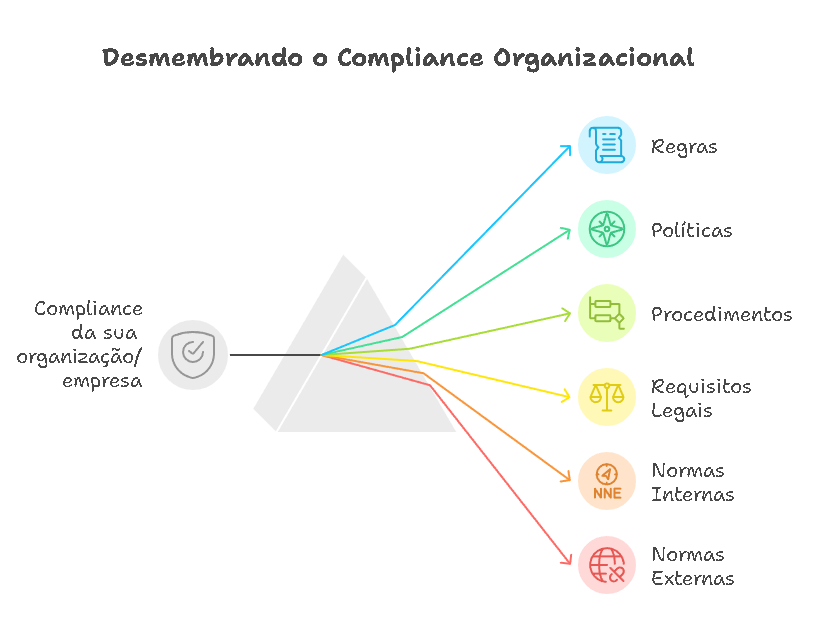
\includegraphics{images/qualidade-geral/compliance.png}

\section{QUALIDADE}\label{qualidade}

O que é Qualidade ? (Definição ISO 9000)

\begin{quote}
Qualidade é definida como o grau em que um conjunto de características inerentes de um objeto satisfaz requisitos onde: \textbf{Características inerentes} São propriedades que fazem parte do objeto, onde:

\begin{itemize}
\item
  \textbf{Requisitos}: São as necessidades ou expectativas declaradas, geralmente implícitas ou obrigatórias;
\item
  \textbf{objeto} pode ser representado por um produto, serviço, processo, organização, sistema ou pessoa;
\end{itemize}
\end{quote}

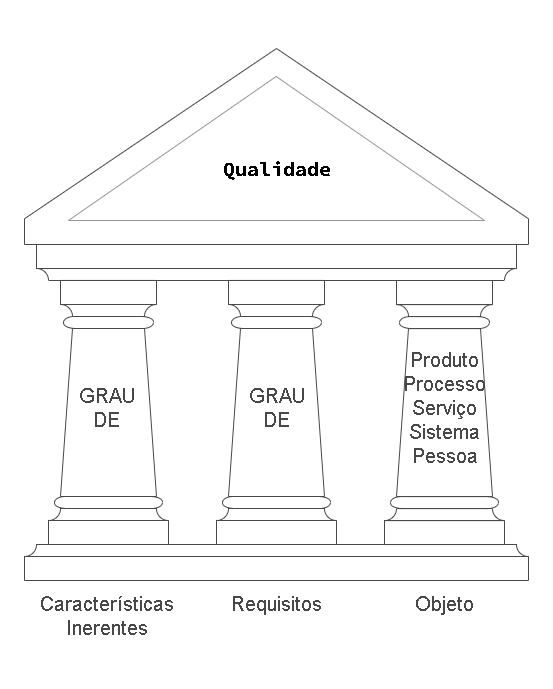
\includegraphics{images/qualidade-geral/Qualidade.png}

\subsection{QUALIDADE APLICADA A PRODUTO}\label{qualidade-aplicada-a-produto}

O CONTROLE DE QUALIDADE do PRODUTO concentra-se em aperfeiçoar:

\begin{itemize}
\item
  as \textbf{características} e
\item
  o \textbf{desempenho} do produto em si,
\end{itemize}

visando atender às necessidades e expectativas dos clientes.

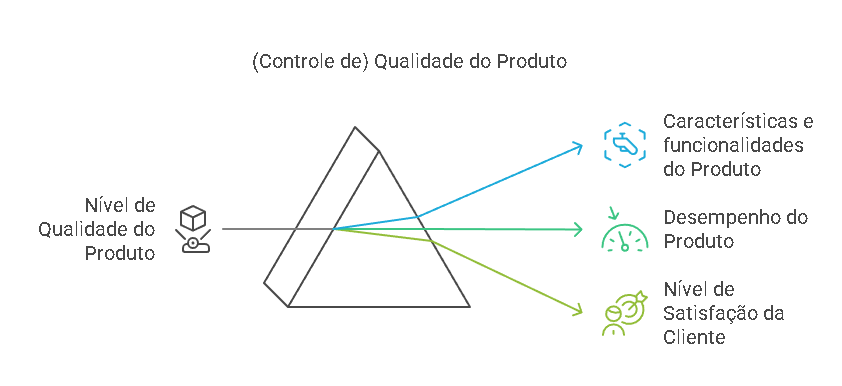
\includegraphics{images/qualidade-geral/Qualidade_do_Produto.png}

\begin{longtable}[]{@{}
  >{\raggedright\arraybackslash}p{(\columnwidth - 0\tabcolsep) * \real{1.0000}}@{}}
\caption{Resultado esperado do CONTROLE DE QUALIDADE aplicado ao PRODUTO}\tabularnewline
\toprule\noalign{}
\begin{minipage}[b]{\linewidth}\raggedright
Resultados do CONTROLE DE QUALIDADE aplicado ao PRODUTO
\end{minipage} \\
\midrule\noalign{}
\endfirsthead
\toprule\noalign{}
\begin{minipage}[b]{\linewidth}\raggedright
Resultados do CONTROLE DE QUALIDADE aplicado ao PRODUTO
\end{minipage} \\
\midrule\noalign{}
\endhead
\bottomrule\noalign{}
\endlastfoot
\begin{minipage}[t]{\linewidth}\raggedright
\begin{itemize}
\tightlist
\item
  Aumento no GRAU das características e funcionalidades do produto.
\end{itemize}
\end{minipage} \\
\begin{minipage}[t]{\linewidth}\raggedright
\begin{itemize}
\tightlist
\item
  Aumento no GRAU de desempenho do produto.
\end{itemize}
\end{minipage} \\
\begin{minipage}[t]{\linewidth}\raggedright
\begin{itemize}
\tightlist
\item
  Aumento no GRAU de nível de satisfação do cliente.
\end{itemize}
\end{minipage} \\
\end{longtable}

\subsection{QUALIDADE APLICADA A PROCESSO}\label{qualidade-aplicada-a-processo}

O CONTROLE DE QUALIDADE DE PROCESSO concentra-se em aperfeiçoar

\begin{itemize}
\item
  as \textbf{atividades} e
\item
  melhor \textbf{aplicação dos recursos}
\end{itemize}

utilizados para criar o produto, visando garantir a consistência e a eficácia da produção.

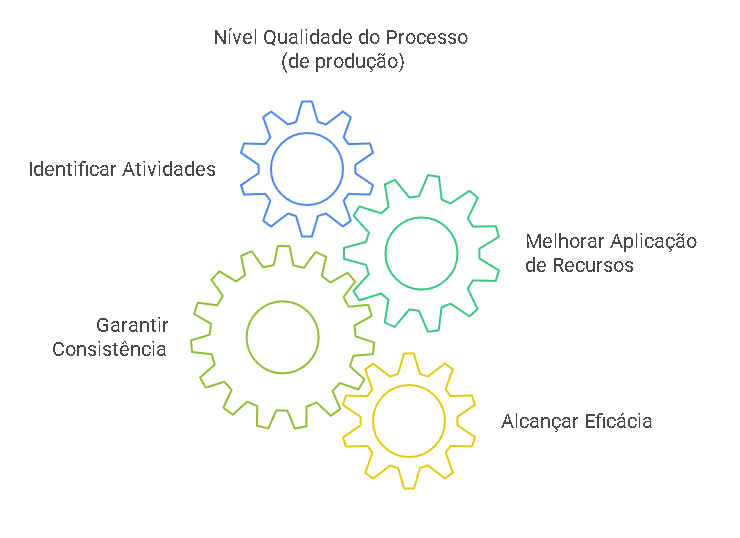
\includegraphics{images/qualidade-geral/Qualidade_do_Processo.png}

\begin{longtable}[]{@{}
  >{\raggedright\arraybackslash}p{(\columnwidth - 0\tabcolsep) * \real{0.8472}}@{}}
\toprule\noalign{}
\begin{minipage}[b]{\linewidth}\raggedright
Resultados do CONTROLE DE QUALIDADE aplicado ao PROCESSO
\end{minipage} \\
\midrule\noalign{}
\endhead
\bottomrule\noalign{}
\endlastfoot
\begin{minipage}[t]{\linewidth}\raggedright
\begin{itemize}
\tightlist
\item
  \textbf{identificar} as ATIVIDADES do processo.
\end{itemize}
\end{minipage} \\
\begin{minipage}[t]{\linewidth}\raggedright
\begin{itemize}
\tightlist
\item
  \textbf{Garantir a Consistência} as ATIVIDADES do processo.
\end{itemize}
\end{minipage} \\
\begin{minipage}[t]{\linewidth}\raggedright
\begin{itemize}
\tightlist
\item
  \textbf{Melhorar} a APLICAÇÃO DE RECURSOS do processo.
\end{itemize}
\end{minipage} \\
\begin{minipage}[t]{\linewidth}\raggedright
\begin{itemize}
\tightlist
\item
  Alcançar a \textbf{EFICÁCIA.}
\end{itemize}
\end{minipage} \\
\end{longtable}

\subsection{CASO MACDONALDS - Qualidade de Produto e Processo}\label{caso-macdonalds---qualidade-de-produto-e-processo}

O filme ``Fome de Poder'' (``The Founder'', no original) narra a história real da ascensão da rede McDonald's, desde sua origem como uma pequena hamburgueria na Califórnia até se tornar um império global do fast-food.

\begin{itemize}
\tightlist
\item
  Reconhecimento da \textbf{qualidade do produto} - hamburguers McDonalds
\end{itemize}

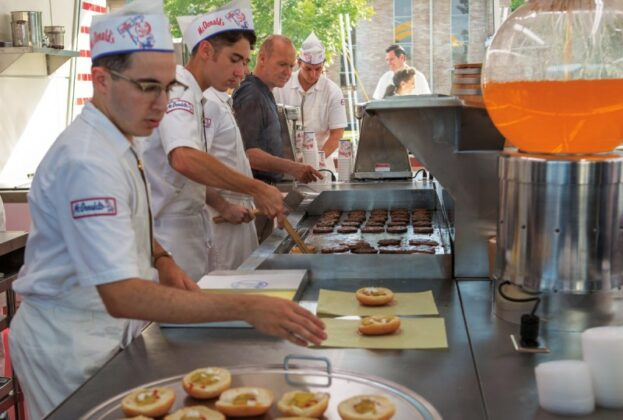
\includegraphics{images/mac-donalds/cozinha-mac.jpg}

Reconhecimento da \textbf{Qualidade do Processo} de fabricação do Produto

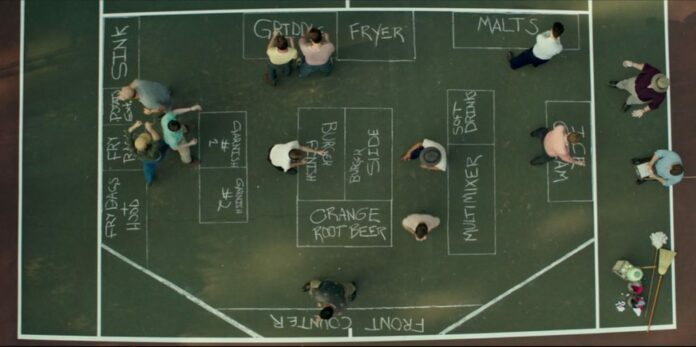
\includegraphics{images/mac-donalds/modelo-mac.jpg}

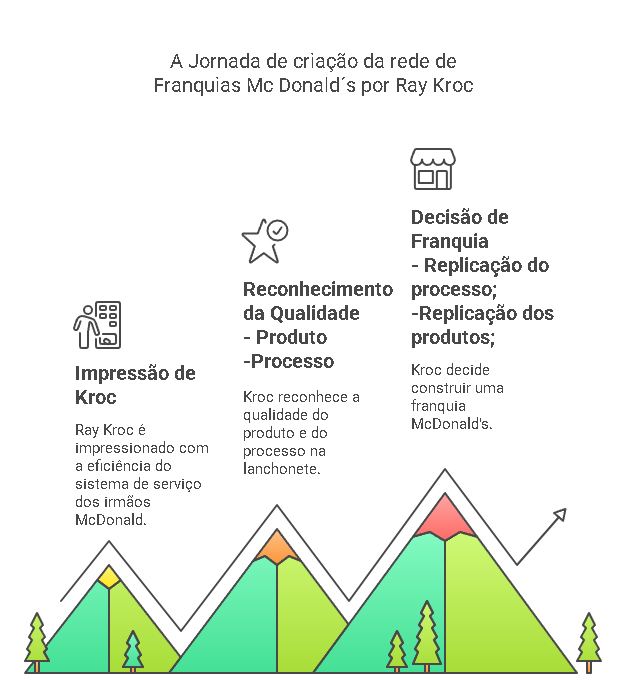
\includegraphics{images/qualidade-geral/MacDonalds1.png}

\begin{itemize}
\tightlist
\item
  Reconhecimento da Capacidade de Franquia (Replicação):
\end{itemize}

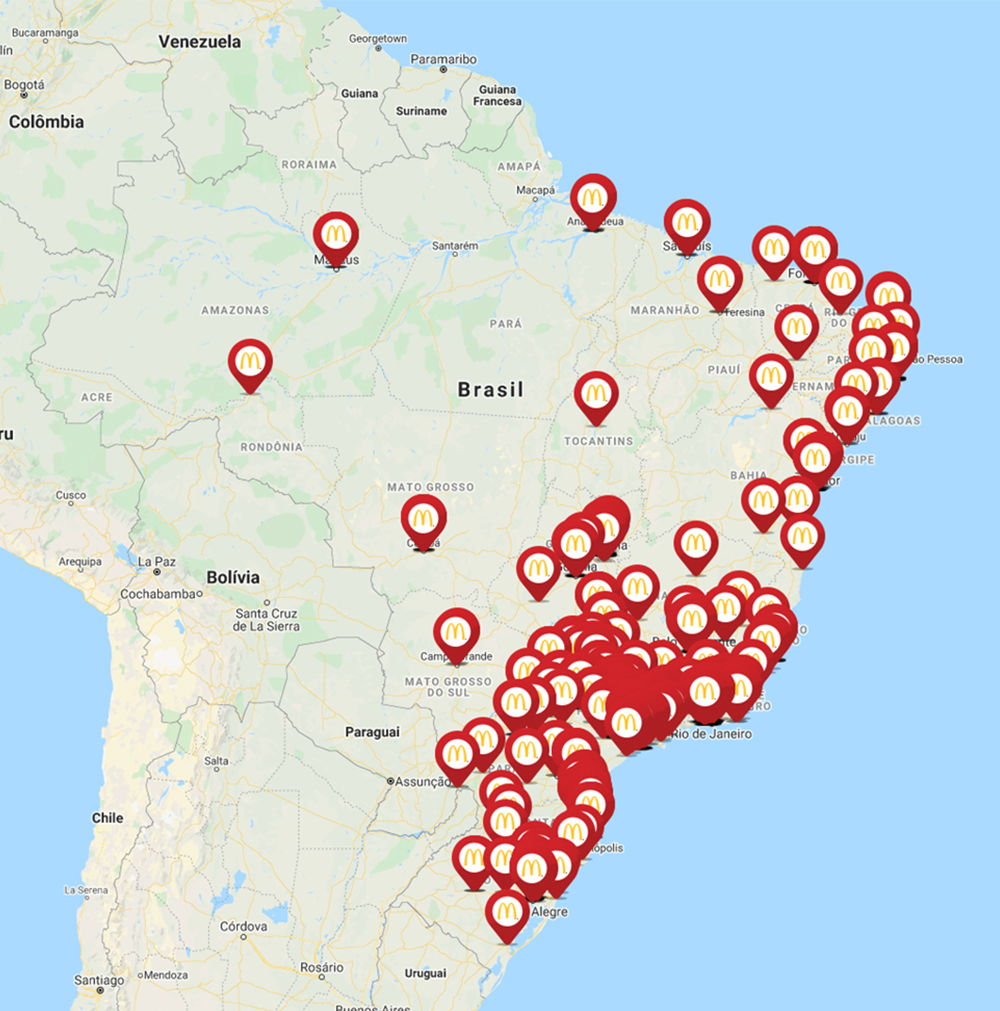
\includegraphics[width=4.23958in,height=\textheight]{images/mac-donalds/Franquias.jpg}

\subsection{QUALIDADE NAS ORGANIZAÇÕES}\label{qualidade-nas-organizauxe7uxf5es}

\subsection{Família ISO 9000}\label{famuxedlia-iso-9000}

\textbf{A NBR ISO 9000} é um conjunto de normas técnicas que estabelecem diretrizes e padrões para a criação de um \textbf{Sistema de Gestão da Qualidade (SGQ)}.

O sistema SGQ (um si que pode ou não ser um pacote de software) deve mapear

\begin{longtable}[]{@{}
  >{\centering\arraybackslash}p{(\columnwidth - 8\tabcolsep) * \real{0.2000}}
  >{\centering\arraybackslash}p{(\columnwidth - 8\tabcolsep) * \real{0.2000}}
  >{\centering\arraybackslash}p{(\columnwidth - 8\tabcolsep) * \real{0.2000}}
  >{\centering\arraybackslash}p{(\columnwidth - 8\tabcolsep) * \real{0.2000}}
  >{\centering\arraybackslash}p{(\columnwidth - 8\tabcolsep) * \real{0.2000}}@{}}
\toprule\noalign{}
\endhead
\bottomrule\noalign{}
\endlastfoot
Áreas mapeadas por um sistema SGQ & PROCESSOS & POLÍTICAS & PROCEDIMENTOS & RESPONSABILIDADES \\
\end{longtable}

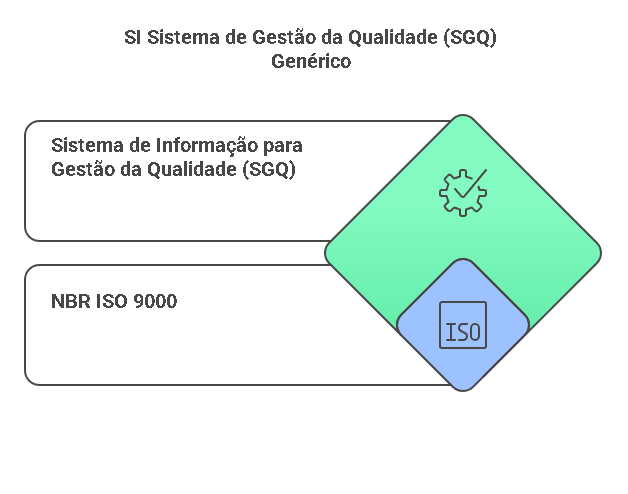
\includegraphics[width=5.71875in,height=\textheight]{images/qualidade-geral/ISO-9000-SGQ.png}

\subsection{Família ISO 14000}\label{famuxedlia-iso-14000}

\textbf{A NBR ISO 14000} é um conjunto de normas técnicas que tratam de GESTÃO AMBIENTAL nas organizações. Estabelecem normas e diretrizes para criar \textbf{(SI) Sistemas de Gestão Ambiental (SGA)}:

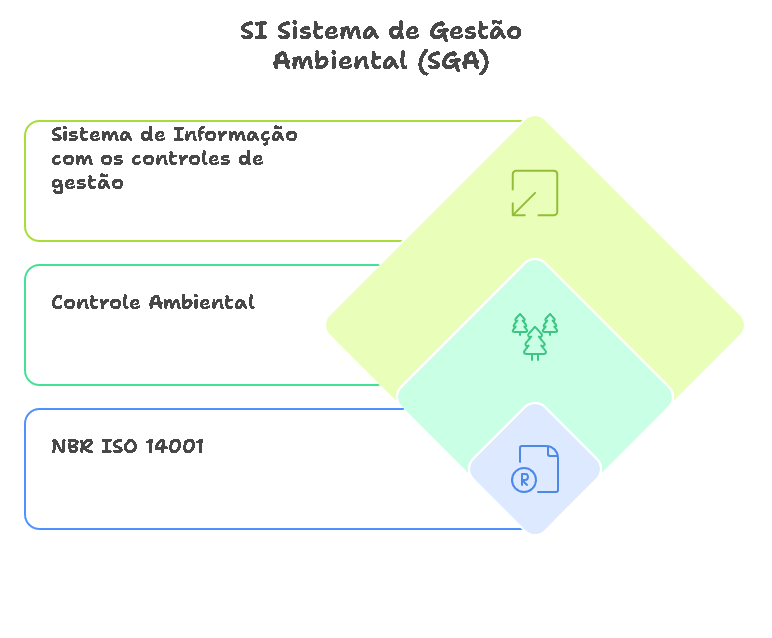
\includegraphics{images/qualidade-geral/ISO-14000-SGQ.png}

\subsection{Família ISO 27000}\label{famuxedlia-iso-27000}

\textbf{NBR ISO 27000}, trata de normas para \textbf{gestão segurança da Informação.} Fornecem um framework para a gestão da segurança da informação em organizações.

Especifica os requisitos para um para a criação de um(SI) Sistema de Gestão de Segurança da Informação (SGSI).

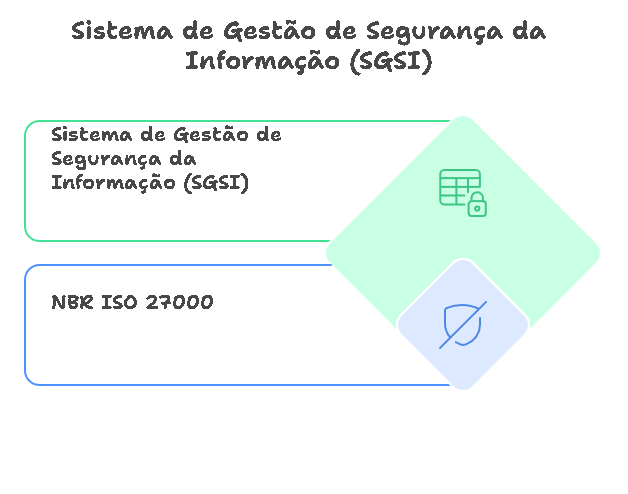
\includegraphics{images/qualidade-geral/ISO-27000-SGSI.png}

\subsection{Segmentos das Organizações e Adoção das normas de Qualidade}\label{segmentos-das-organizauxe7uxf5es-e-adouxe7uxe3o-das-normas-de-qualidade}

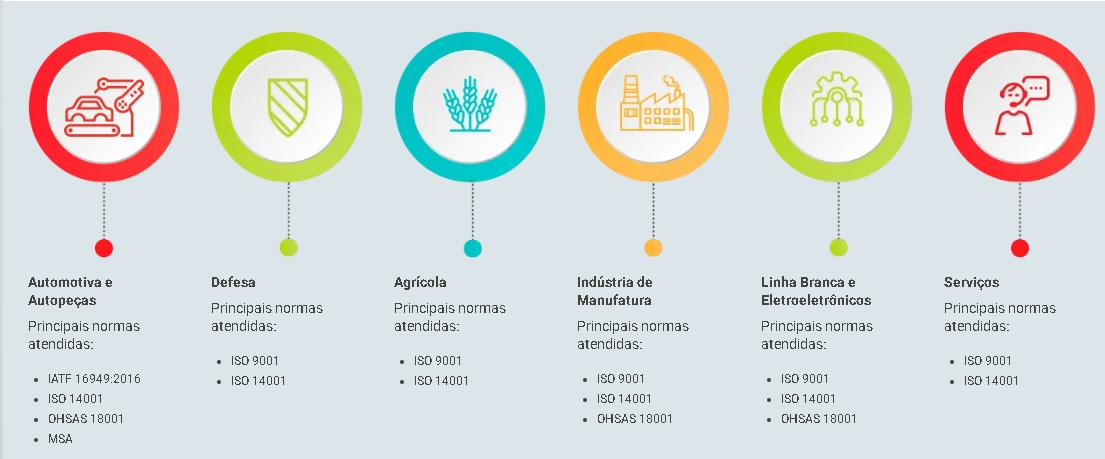
\includegraphics{images/qualidade-geral/segmentos.jpg}

\subsection{QUALIDADE NA ENGENHARIA DE SOFTWARE}\label{qualidade-na-engenharia-de-software}

A qualidade de software não define S.I.s

\subsection{Família NBR ISO 9126}\label{famuxedlia-nbr-iso-9126}

Focava na qualidade do produto de software, definindo um conjunto de parâmetros para padronizar a avaliação dessa qualidade. Ela se enquadrava no modelo de qualidade das normas da família 9000.

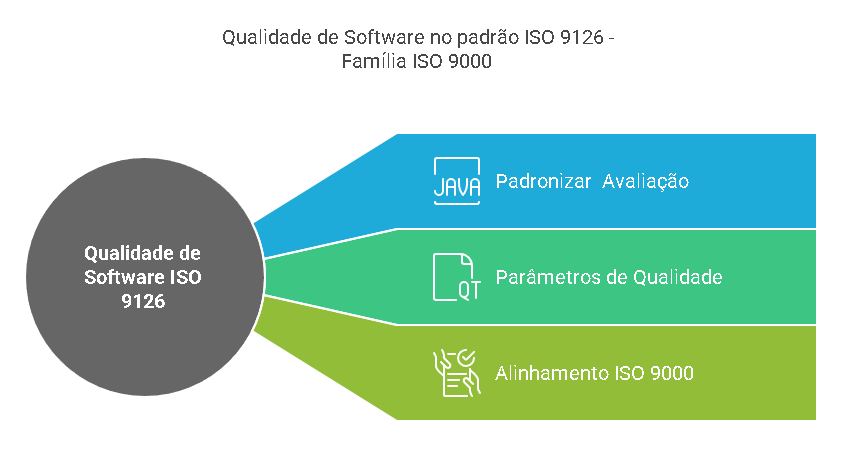
\includegraphics{images/qualidade-geral/ISO-9126-SGSI.png}

\subsection{Família NBR ISO 12207}\label{famuxedlia-nbr-iso-12207}

A norma ISO 12207 define um conjunto de processos para o ciclo de vida do software. Seu principal foco é estabelecer um framework padronizado para o desenvolvimento, manutenção e descarte de software, visando garantir a qualidade e a eficiência desses processos.

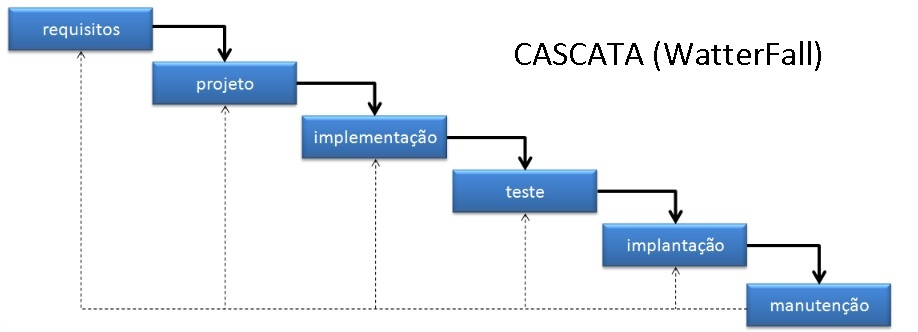
\includegraphics{images/modelos_processos_software/Cascata.jpg}

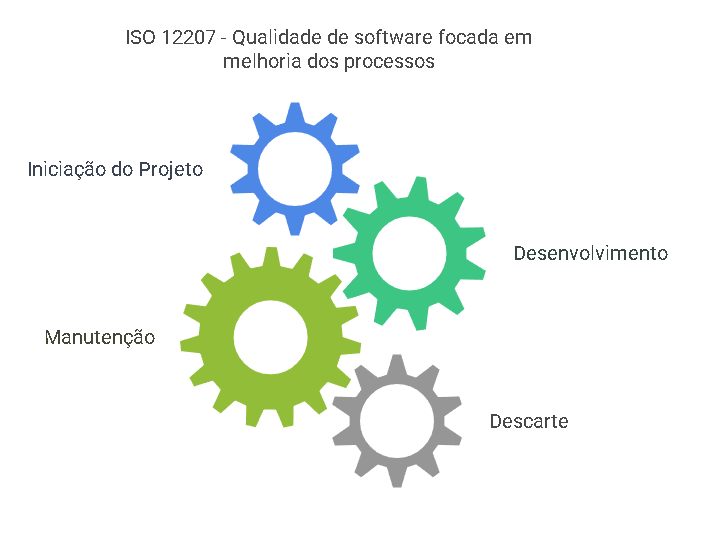
\includegraphics{images/qualidade-geral/ISO-12207-processos.png}

\subsection{Família NBR ISO 25000}\label{famuxedlia-nbr-iso-25000}

\textbf{A NBR ISO 25000}, também conhecida como SQuaRE (Software Product Quality Requirements and Evaluation - Requisitos e Avaliação da Qualidade de Produtos de Software), é uma série de normas internacionais que fornecem um subconjunto de normas para a avaliação da qualidade de produtos de software. Este subconjunto é formado pelas normas \textbf{ISO/IEC 25000} , \textbf{ISO/IEC 25010}, \textbf{ISO/IEC 25020}, \textbf{ISO/IEC 25030} e \textbf{ISO/IEC 25040}.

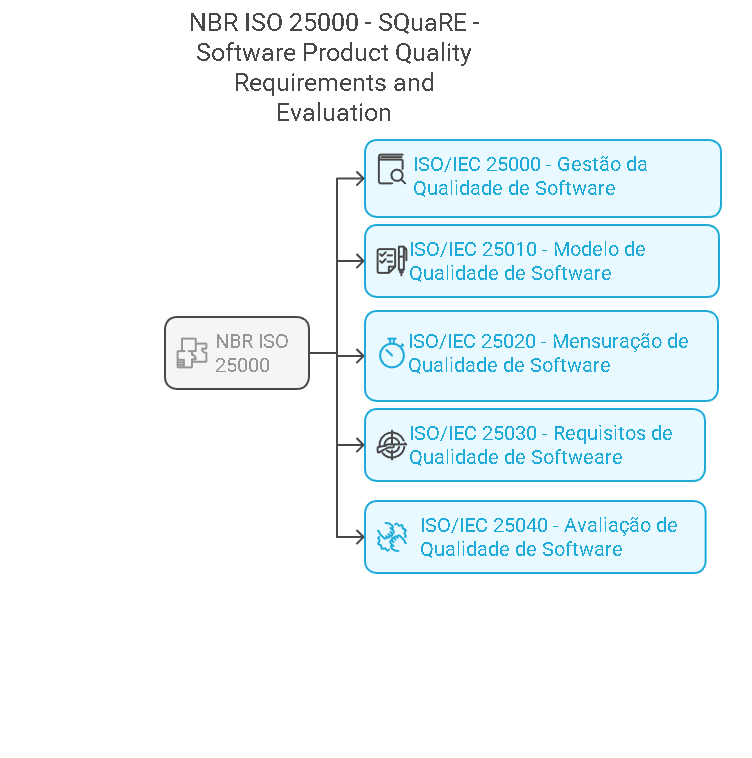
\includegraphics{images/qualidade-geral/ISO-25000-SQuaRE.png}

\section{Exercício de Fixação:}\label{exercuxedcio-de-fixauxe7uxe3o}

\subsection{Testes:}\label{testes}

\begin{longtable}[]{@{}
  >{\raggedright\arraybackslash}p{(\columnwidth - 0\tabcolsep) * \real{1.0085}}@{}}
\toprule\noalign{}
\begin{minipage}[b]{\linewidth}\raggedright
TESTE 01
\end{minipage} \\
\midrule\noalign{}
\endhead
\bottomrule\noalign{}
\endlastfoot
\textbf{Qual das seguintes alternativas melhor descreve o conceito de qualidade, de acordo com a definição apresentada?} \\
\begin{minipage}[t]{\linewidth}\raggedright
\begin{enumerate}
\def\labelenumi{\alph{enumi})}
\tightlist
\item
  Qualidade é a ausência de defeitos em um produto ou serviço.
\end{enumerate}
\end{minipage} \\
\begin{minipage}[t]{\linewidth}\raggedright
\begin{enumerate}
\def\labelenumi{\alph{enumi})}
\setcounter{enumi}{1}
\tightlist
\item
  Qualidade é o grau em que um produto ou serviço excede as expectativas do cliente.
\end{enumerate}
\end{minipage} \\
\begin{minipage}[t]{\linewidth}\raggedright
\begin{enumerate}
\def\labelenumi{\alph{enumi})}
\setcounter{enumi}{2}
\tightlist
\item
  Qualidade é o grau em que um conjunto de características inerentes de um objeto satisfaz requisitos.
\end{enumerate}
\end{minipage} \\
\begin{minipage}[t]{\linewidth}\raggedright
\begin{enumerate}
\def\labelenumi{\alph{enumi})}
\setcounter{enumi}{3}
\tightlist
\item
  Qualidade é a conformidade com as normas e regulamentos estabelecidos.
\end{enumerate}
\end{minipage} \\
\begin{minipage}[t]{\linewidth}\raggedright
\begin{enumerate}
\def\labelenumi{\alph{enumi})}
\setcounter{enumi}{4}
\tightlist
\item
  Qualidade é a capacidade de um produto ou serviço ser produzido em grande quantidade.
\end{enumerate}
\end{minipage} \\
\end{longtable}

\begin{longtable}[]{@{}
  >{\raggedright\arraybackslash}p{(\columnwidth - 0\tabcolsep) * \real{1.0067}}@{}}
\toprule\noalign{}
\begin{minipage}[b]{\linewidth}\raggedright
TESTE 02
\end{minipage} \\
\midrule\noalign{}
\endhead
\bottomrule\noalign{}
\endlastfoot
\textbf{Qual das seguintes alternativas melhor descreve o conceito de Compliance?} \\
\begin{minipage}[t]{\linewidth}\raggedright
\begin{enumerate}
\def\labelenumi{\alph{enumi})}
\tightlist
\item
  Compliance é um conjunto de estratégias de marketing para aumentar a visibilidade da empresa.
\end{enumerate}
\end{minipage} \\
\begin{minipage}[t]{\linewidth}\raggedright
\begin{enumerate}
\def\labelenumi{\alph{enumi})}
\setcounter{enumi}{1}
\tightlist
\item
  Compliance é um sistema de gestão financeira para otimizar os lucros da empresa.
\end{enumerate}
\end{minipage} \\
\begin{minipage}[t]{\linewidth}\raggedright
\begin{enumerate}
\def\labelenumi{\alph{enumi})}
\setcounter{enumi}{2}
\tightlist
\item
  Compliance é o conjunto de normas, procedimentos e práticas para cumprir legislação e padrões éticos, visando segurança e minimização de riscos.
\end{enumerate}
\end{minipage} \\
\begin{minipage}[t]{\linewidth}\raggedright
\begin{enumerate}
\def\labelenumi{\alph{enumi})}
\setcounter{enumi}{3}
\tightlist
\item
  Compliance é um programa de treinamento para melhorar o desempenho dos funcionários.
\end{enumerate}
\end{minipage} \\
\begin{minipage}[t]{\linewidth}\raggedright
\begin{enumerate}
\def\labelenumi{\alph{enumi})}
\setcounter{enumi}{4}
\tightlist
\item
  Compliance é uma ferramenta de análise de mercado para identificar oportunidades de negócio.
\end{enumerate}
\end{minipage} \\
\end{longtable}

\begin{longtable}[]{@{}
  >{\raggedright\arraybackslash}p{(\columnwidth - 0\tabcolsep) * \real{1.0068}}@{}}
\toprule\noalign{}
\begin{minipage}[b]{\linewidth}\raggedright
TESTE 03
\end{minipage} \\
\midrule\noalign{}
\endhead
\bottomrule\noalign{}
\endlastfoot
\textbf{Qual das seguintes alternativas melhor descreve o conceito de qualidade aplicada ao produto?} \\
\begin{minipage}[t]{\linewidth}\raggedright
\begin{enumerate}
\def\labelenumi{\alph{enumi})}
\tightlist
\item
  Qualidade do produto é a capacidade de um produto ser vendido a um preço baixo.
\end{enumerate}
\end{minipage} \\
\begin{minipage}[t]{\linewidth}\raggedright
\begin{enumerate}
\def\labelenumi{\alph{enumi})}
\setcounter{enumi}{1}
\tightlist
\item
  Qualidade do produto é o grau em que um produto atende às expectativas do cliente em relação às suas características inerentes e o desempenho.
\end{enumerate}
\end{minipage} \\
\begin{minipage}[t]{\linewidth}\raggedright
\begin{enumerate}
\def\labelenumi{\alph{enumi})}
\setcounter{enumi}{2}
\tightlist
\item
  Qualidade do produto é a quantidade de produtos produzidos em um determinado período de tempo.
\end{enumerate}
\end{minipage} \\
\begin{minipage}[t]{\linewidth}\raggedright
\begin{enumerate}
\def\labelenumi{\alph{enumi})}
\setcounter{enumi}{3}
\tightlist
\item
  Qualidade do produto é a aparência estética de um produto, independentemente de sua funcionalidade.
\end{enumerate}
\end{minipage} \\
\begin{minipage}[t]{\linewidth}\raggedright
\begin{enumerate}
\def\labelenumi{\alph{enumi})}
\setcounter{enumi}{4}
\tightlist
\item
  Qualidade do produto é a capacidade de um produto ser facilmente descartado após o uso.
\end{enumerate}
\end{minipage} \\
\end{longtable}

\begin{longtable}[]{@{}
  >{\raggedright\arraybackslash}p{(\columnwidth - 0\tabcolsep) * \real{1.0069}}@{}}
\toprule\noalign{}
\begin{minipage}[b]{\linewidth}\raggedright
TESTE 04
\end{minipage} \\
\midrule\noalign{}
\endhead
\bottomrule\noalign{}
\endlastfoot
\textbf{Qual das seguintes alternativas melhor descreve o conceito de qualidade aplicada ao processo?} \\
\begin{minipage}[t]{\linewidth}\raggedright
\begin{enumerate}
\def\labelenumi{\alph{enumi})}
\tightlist
\item
  Qualidade no processo se refere à inspeção final do produto para garantir que ele esteja livre de defeitos.
\end{enumerate}
\end{minipage} \\
\begin{minipage}[t]{\linewidth}\raggedright
\begin{enumerate}
\def\labelenumi{\alph{enumi})}
\setcounter{enumi}{1}
\tightlist
\item
  Qualidade no processo é a capacidade de um processo produzir resultados consistentes e previsíveis, atendendo aos requisitos estabelecidos.
\end{enumerate}
\end{minipage} \\
\begin{minipage}[t]{\linewidth}\raggedright
\begin{enumerate}
\def\labelenumi{\alph{enumi})}
\setcounter{enumi}{2}
\tightlist
\item
  Qualidade no processo é a utilização de materiais de alta qualidade na fabricação do produto.
\end{enumerate}
\end{minipage} \\
\begin{minipage}[t]{\linewidth}\raggedright
\begin{enumerate}
\def\labelenumi{\alph{enumi})}
\setcounter{enumi}{3}
\tightlist
\item
  Qualidade no processo é a implementação de um sistema de gestão da qualidade certificado, como a ISO 9001.
\end{enumerate}
\end{minipage} \\
\begin{minipage}[t]{\linewidth}\raggedright
\begin{enumerate}
\def\labelenumi{\alph{enumi})}
\setcounter{enumi}{4}
\tightlist
\item
  Qualidade no processo é a satisfação do cliente com o produto final, independentemente de como ele foi produzido.
\end{enumerate}
\end{minipage} \\
\end{longtable}

\begin{longtable}[]{@{}
  >{\raggedright\arraybackslash}p{(\columnwidth - 0\tabcolsep) * \real{1.0061}}@{}}
\toprule\noalign{}
\begin{minipage}[b]{\linewidth}\raggedright
TESTE 05
\end{minipage} \\
\midrule\noalign{}
\endhead
\bottomrule\noalign{}
\endlastfoot
\textbf{Quais das alternativas melhor reflete principais resultados do controle de qualidade aplicado ao produto?} \\
\begin{minipage}[t]{\linewidth}\raggedright
\begin{enumerate}
\def\labelenumi{\alph{enumi})}
\tightlist
\item
  Aumento no grau das características e funcionalidades do produto, aumento no grau de desempenho do produto e aumento no grau de nível de satisfação do cliente.
\end{enumerate}
\end{minipage} \\
\begin{minipage}[t]{\linewidth}\raggedright
\begin{enumerate}
\def\labelenumi{\alph{enumi})}
\setcounter{enumi}{1}
\tightlist
\item
  Redução de custos de produção, aumento da eficiência dos processos e diminuição do tempo de entrega.
\end{enumerate}
\end{minipage} \\
\begin{minipage}[t]{\linewidth}\raggedright
\begin{enumerate}
\def\labelenumi{\alph{enumi})}
\setcounter{enumi}{2}
\tightlist
\item
  Melhoria na imagem da empresa, aumento da participação de mercado e expansão para novos mercados.
\end{enumerate}
\end{minipage} \\
\begin{minipage}[t]{\linewidth}\raggedright
\begin{enumerate}
\def\labelenumi{\alph{enumi})}
\setcounter{enumi}{3}
\tightlist
\item
  Padronização dos produtos, simplificação dos processos de fabricação e redução do desperdício de materiais.
\end{enumerate}
\end{minipage} \\
\begin{minipage}[t]{\linewidth}\raggedright
\begin{enumerate}
\def\labelenumi{\alph{enumi})}
\setcounter{enumi}{4}
\tightlist
\item
  Maior flexibilidade na produção, personalização dos produtos e aumento da variedade de produtos oferecidos.
\end{enumerate}
\end{minipage} \\
\end{longtable}

\begin{longtable}[]{@{}
  >{\raggedright\arraybackslash}p{(\columnwidth - 0\tabcolsep) * \real{1.0061}}@{}}
\toprule\noalign{}
\begin{minipage}[b]{\linewidth}\raggedright
TESTE 06
\end{minipage} \\
\midrule\noalign{}
\endhead
\bottomrule\noalign{}
\endlastfoot
\textbf{Qual era o principal objetivo da família de normas ISO/NBR 9126?} \\
\begin{minipage}[t]{\linewidth}\raggedright
\begin{enumerate}
\def\labelenumi{\alph{enumi})}
\tightlist
\item
  Definir padrões para a gestão de projetos de software.
\end{enumerate}
\end{minipage} \\
\begin{minipage}[t]{\linewidth}\raggedright
\begin{enumerate}
\def\labelenumi{\alph{enumi})}
\setcounter{enumi}{1}
\tightlist
\item
  Estabelecer diretrizes para a segurança da informação em sistemas de software.
\end{enumerate}
\end{minipage} \\
\begin{minipage}[t]{\linewidth}\raggedright
\begin{enumerate}
\def\labelenumi{\alph{enumi})}
\setcounter{enumi}{2}
\tightlist
\item
  Padronizar a documentação de software e os processos de desenvolvimento.
\end{enumerate}
\end{minipage} \\
\begin{minipage}[t]{\linewidth}\raggedright
\begin{enumerate}
\def\labelenumi{\alph{enumi})}
\setcounter{enumi}{3}
\tightlist
\item
  Promover a interoperabilidade entre diferentes sistemas de software.
\end{enumerate}
\end{minipage} \\
\begin{minipage}[t]{\linewidth}\raggedright
\begin{enumerate}
\def\labelenumi{\alph{enumi})}
\setcounter{enumi}{4}
\tightlist
\item
  Padronizar a avaliação da qualidade de produtos de software, definindo parâmetros para essa avaliação dentro do modelo de qualidade das normas da família 9000.
\end{enumerate}
\end{minipage} \\
\end{longtable}

\begin{longtable}[]{@{}
  >{\raggedright\arraybackslash}p{(\columnwidth - 0\tabcolsep) * \real{1.0109}}@{}}
\toprule\noalign{}
\endhead
\bottomrule\noalign{}
\endlastfoot
\textbf{TESTE 07} \\
Qual tipo de Sistema de Informação (SI) a família de normas ISO 9000 propunha implementar? \\
\begin{minipage}[t]{\linewidth}\raggedright
\begin{enumerate}
\def\labelenumi{\alph{enumi})}
\tightlist
\item
  Sistema de Gestão Financeira (SGF)
\end{enumerate}
\end{minipage} \\
\begin{minipage}[t]{\linewidth}\raggedright
\begin{enumerate}
\def\labelenumi{\alph{enumi})}
\setcounter{enumi}{1}
\tightlist
\item
  Sistema de Gestão de Recursos Humanos (SGRH)
\end{enumerate}
\end{minipage} \\
\begin{minipage}[t]{\linewidth}\raggedright
\begin{enumerate}
\def\labelenumi{\alph{enumi})}
\setcounter{enumi}{2}
\tightlist
\item
  Sistema de Gestão da Qualidade (SGQ)
\end{enumerate}
\end{minipage} \\
\begin{minipage}[t]{\linewidth}\raggedright
\begin{enumerate}
\def\labelenumi{\alph{enumi})}
\setcounter{enumi}{3}
\tightlist
\item
  Sistema de Gestão de Produção (SGP)
\end{enumerate}
\end{minipage} \\
\begin{minipage}[t]{\linewidth}\raggedright
\begin{enumerate}
\def\labelenumi{\alph{enumi})}
\setcounter{enumi}{4}
\tightlist
\item
  Sistema de Gestão de Marketing (SGM)
\end{enumerate}
\end{minipage} \\
\end{longtable}

\begin{longtable}[]{@{}
  >{\raggedright\arraybackslash}p{(\columnwidth - 0\tabcolsep) * \real{1.0085}}@{}}
\toprule\noalign{}
\begin{minipage}[b]{\linewidth}\raggedright
TESTE 08
\end{minipage} \\
\midrule\noalign{}
\endhead
\bottomrule\noalign{}
\endlastfoot
\textbf{Qual área a família de normas ISO 14000 trata e qual tipo de Sistema de Informação (SI) ela propõe implementar?} \\
\begin{minipage}[t]{\linewidth}\raggedright
\begin{enumerate}
\def\labelenumi{\alph{enumi})}
\tightlist
\item
  Trata da gestão da qualidade e propõe implementar um Sistema de Gestão da Qualidade (SGQ).
\end{enumerate}
\end{minipage} \\
\begin{minipage}[t]{\linewidth}\raggedright
\begin{enumerate}
\def\labelenumi{\alph{enumi})}
\setcounter{enumi}{1}
\tightlist
\item
  Trata da segurança da informação e propõe implementar um Sistema de Gestão de Segurança da Informação (SGSI).
\end{enumerate}
\end{minipage} \\
\begin{minipage}[t]{\linewidth}\raggedright
\begin{enumerate}
\def\labelenumi{\alph{enumi})}
\setcounter{enumi}{2}
\tightlist
\item
  Trata da gestão de projetos e propõe implementar um Sistema de Gestão de Projetos (SGP).
\end{enumerate}
\end{minipage} \\
\begin{minipage}[t]{\linewidth}\raggedright
\begin{enumerate}
\def\labelenumi{\alph{enumi})}
\setcounter{enumi}{3}
\tightlist
\item
  Trata da gestão de recursos humanos e propõe implementar um Sistema de Gestão de Recursos Humanos (SGRH).
\end{enumerate}
\end{minipage} \\
\begin{minipage}[t]{\linewidth}\raggedright
\begin{enumerate}
\def\labelenumi{\alph{enumi})}
\setcounter{enumi}{4}
\tightlist
\item
  Trata da gestão ambiental e propõe implementar um Sistema de Gestão Ambiental (SGA).
\end{enumerate}
\end{minipage} \\
\end{longtable}

\begin{longtable}[]{@{}
  >{\raggedright\arraybackslash}p{(\columnwidth - 0\tabcolsep) * \real{1.0053}}@{}}
\toprule\noalign{}
\begin{minipage}[b]{\linewidth}\raggedright
TESTE 09
\end{minipage} \\
\midrule\noalign{}
\endhead
\bottomrule\noalign{}
\endlastfoot
\textbf{Qual é o principal objetivo da norma ISO 12207?} \\
\begin{minipage}[t]{\linewidth}\raggedright
\begin{enumerate}
\def\labelenumi{\alph{enumi})}
\tightlist
\item
  Definir um conjunto de processos para o ciclo de vida do software, estabelecendo um framework padronizado para desenvolvimento, manutenção e descarte, visando qualidade e eficiência.
\end{enumerate}
\end{minipage} \\
\begin{minipage}[t]{\linewidth}\raggedright
\begin{enumerate}
\def\labelenumi{\alph{enumi})}
\setcounter{enumi}{1}
\tightlist
\item
  Estabelecer diretrizes para a segurança da informação em sistemas de software.
\end{enumerate}
\end{minipage} \\
\begin{minipage}[t]{\linewidth}\raggedright
\begin{enumerate}
\def\labelenumi{\alph{enumi})}
\setcounter{enumi}{2}
\tightlist
\item
  Padronizar a documentação de software e os processos de desenvolvimento ágil.
\end{enumerate}
\end{minipage} \\
\begin{minipage}[t]{\linewidth}\raggedright
\begin{enumerate}
\def\labelenumi{\alph{enumi})}
\setcounter{enumi}{3}
\tightlist
\item
  Promover a interoperabilidade entre diferentes sistemas de software e hardware.
\end{enumerate}
\end{minipage} \\
\begin{minipage}[t]{\linewidth}\raggedright
\begin{enumerate}
\def\labelenumi{\alph{enumi})}
\setcounter{enumi}{4}
\tightlist
\item
  Definir padrões para a gestão de projetos de software, focando na otimização de custos e prazos.
\end{enumerate}
\end{minipage} \\
\end{longtable}

\begin{longtable}[]{@{}
  >{\raggedright\arraybackslash}p{(\columnwidth - 0\tabcolsep) * \real{1.0119}}@{}}
\toprule\noalign{}
\begin{minipage}[b]{\linewidth}\raggedright
TESTE 10
\end{minipage} \\
\midrule\noalign{}
\endhead
\bottomrule\noalign{}
\endlastfoot
\textbf{Qual é o principal objetivo da família de normas NBR ISO 25000 (SQuaRE)?} \\
\begin{minipage}[t]{\linewidth}\raggedright
\begin{enumerate}
\def\labelenumi{\alph{enumi})}
\tightlist
\item
  Definir padrões para a gestão de projetos de software.
\end{enumerate}
\end{minipage} \\
\begin{minipage}[t]{\linewidth}\raggedright
\begin{enumerate}
\def\labelenumi{\alph{enumi})}
\setcounter{enumi}{1}
\tightlist
\item
  Estabelecer diretrizes para a segurança da informação em sistemas de software.
\end{enumerate}
\end{minipage} \\
\begin{minipage}[t]{\linewidth}\raggedright
\begin{enumerate}
\def\labelenumi{\alph{enumi})}
\setcounter{enumi}{2}
\tightlist
\item
  Padronizar a avaliação da qualidade de produtos de software.
\end{enumerate}
\end{minipage} \\
\begin{minipage}[t]{\linewidth}\raggedright
\begin{enumerate}
\def\labelenumi{\alph{enumi})}
\setcounter{enumi}{3}
\tightlist
\item
  Promover a interoperabilidade entre diferentes sistemas de software.
\end{enumerate}
\end{minipage} \\
\begin{minipage}[t]{\linewidth}\raggedright
\begin{enumerate}
\def\labelenumi{\alph{enumi})}
\setcounter{enumi}{4}
\tightlist
\item
  Definir processos para o ciclo de vida do software.
\end{enumerate}
\end{minipage} \\
\end{longtable}

\begin{longtable}[]{@{}
  >{\raggedright\arraybackslash}p{(\columnwidth - 0\tabcolsep) * \real{1.0000}}@{}}
\toprule\noalign{}
\begin{minipage}[b]{\linewidth}\raggedright
TESTE 11
\end{minipage} \\
\midrule\noalign{}
\endhead
\bottomrule\noalign{}
\endlastfoot
Qual subnorma da NBR ISO 25000 (SQuaRE) é responsável por definir modelos de qualidade para produtos de software? \\
Alternativas: \\
a) ISO/IEC 25020 \\
b) ISO/IEC 25030 \\
c) ISO/IEC 25040 \\
d) ISO/IEC 25010 \\
e) ISO/IEC 25000 \\
\end{longtable}

\begin{longtable}[]{@{}
  >{\raggedright\arraybackslash}p{(\columnwidth - 0\tabcolsep) * \real{1.0000}}@{}}
\toprule\noalign{}
\begin{minipage}[b]{\linewidth}\raggedright
TESTE 12
\end{minipage} \\
\midrule\noalign{}
\endhead
\bottomrule\noalign{}
\endlastfoot
Qual subnorma da NBR ISO 25000 (SQuaRE) fornece diretrizes para a avaliação da qualidade de produtos de software? \\
a) ISO/IEC 25040 \\
b) ISO/IEC 25020 \\
c) ISO/IEC 25030 \\
d) ISO/IEC 25010 \\
e) ISO/IEC 25000 \\
\end{longtable}

\subsection{Repostas dos testes}\label{repostas-dos-testes}

\begin{longtable}[]{@{}lc@{}}
\toprule\noalign{}
Teste & Alternativa Correta \\
\midrule\noalign{}
\endhead
\bottomrule\noalign{}
\endlastfoot
01 & c \\
02 & c \\
03 & b \\
04 & b \\
05 & a \\
06 & e \\
07 & c \\
08 & e \\
09 & a \\
10 & c \\
11 & d \\
12 & a \\
\end{longtable}

\chapter{Verificação de Validação de Software}\label{verificauxe7uxe3o-de-validauxe7uxe3o-de-software}

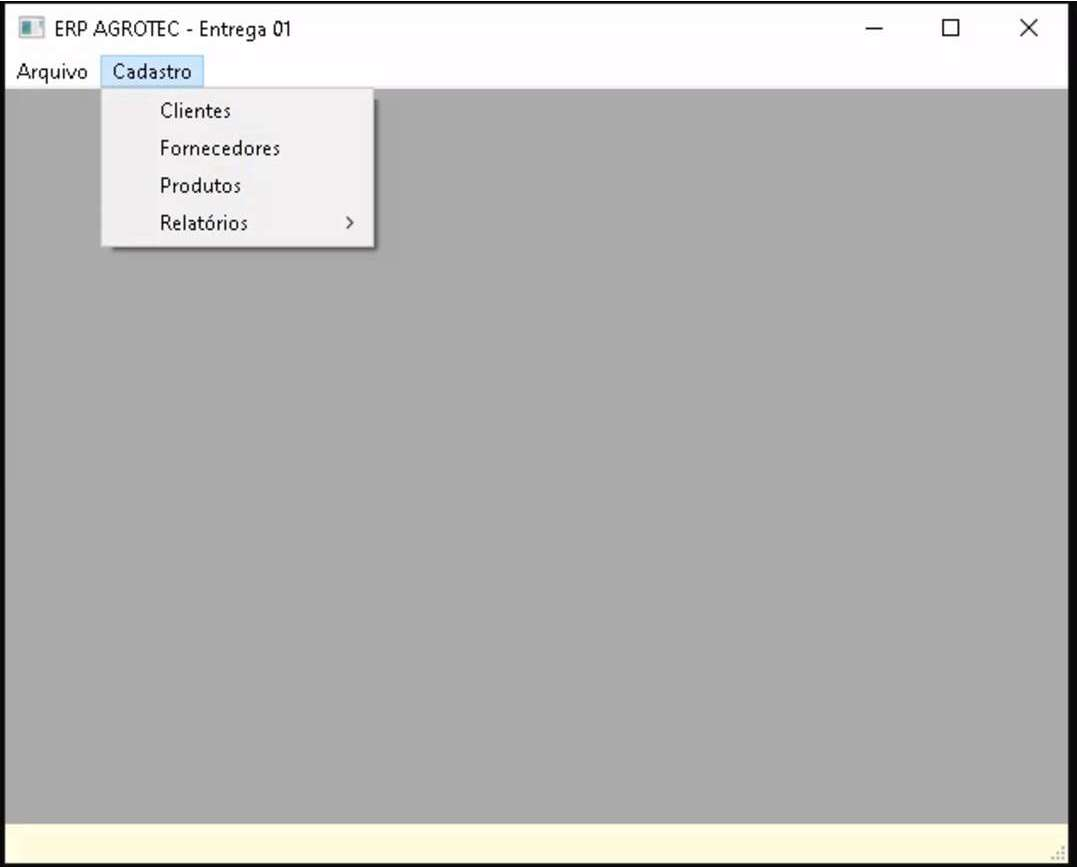
\includegraphics{images/agrotech.jpg}

Conforme sabemos existem quatro \textbf{atividades} fundamentais no \textbf{processo de engenharia de software}. Estas atividades podem ser organizadas de diferentes maneiras dependendo do processo de desenvolvimento utilizado. A seguinte tabela resume as atividades do processo de software de acordo com Sommerville:

\begin{longtable}[]{@{}
  >{\raggedright\arraybackslash}p{(\columnwidth - 2\tabcolsep) * \real{0.5000}}
  >{\raggedright\arraybackslash}p{(\columnwidth - 2\tabcolsep) * \real{0.5000}}@{}}
\toprule\noalign{}
\begin{minipage}[b]{\linewidth}\raggedright
Atividade do Processo de Software
\end{minipage} & \begin{minipage}[b]{\linewidth}\raggedright
Descrição
\end{minipage} \\
\midrule\noalign{}
\endhead
\bottomrule\noalign{}
\endlastfoot
\emph{Especificação de Software} & \emph{A funcionalidade do software e as restrições ao seu funcionamento devem ser definidas.} \\
\emph{Projeto e Implementação de Software} & \emph{O software deve ser produzido para atender às especificações.} \\
\textbf{Validação de Software} & \textbf{O software deve ser validado para garantir que atenda às demandas do cliente.} \\
\emph{Evolução de Software} & \emph{O software deve evoluir para atender às necessidades de mudança dos clientes. Alterações no software são uma parte inevitável.} \\
\end{longtable}

Hoje vamos explorar a terceira etapa, mas especificamente a \emph{Verificação e Validação de Software}.

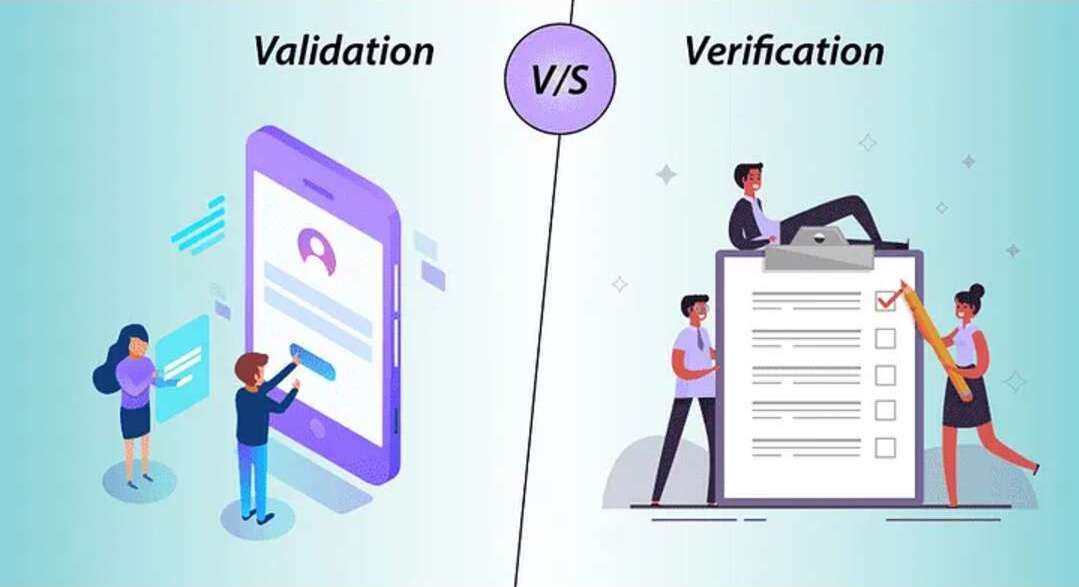
\includegraphics{images/verificacao-validacao.jpg}

\section{Verificação de Software:}\label{verificauxe7uxe3o-de-software}

\begin{quote}
\textbf{Definição de Verificação de Software}: \emph{Assegurar que o software implementa corretamente uma função específica. ``Estamos criando o produto corretamente?}''.
\end{quote}

\section{Validação de Software:}\label{validauxe7uxe3o-de-software}

\begin{quote}
\textbf{Definição de Validação de Software}: \emph{Assegurar que o software foi criado e pode ser rastreado segundo os requisitos do cliente. ``Estamos criando o produto certo?''. Validação tem sucesso quando o software funciona de uma maneira que pode ser razoavelmente esperada pelo cliente.}
\end{quote}

Quais os objetivos globais da etapa de Verificação e Validação de Software ?

\begin{longtable}[]{@{}
  >{\raggedright\arraybackslash}p{(\columnwidth - 0\tabcolsep) * \real{1.0116}}@{}}
\toprule\noalign{}
\begin{minipage}[b]{\linewidth}\raggedright
Objetivos Globais - Etapa de Verificação e Validação do Processo de Software
\end{minipage} \\
\midrule\noalign{}
\endhead
\bottomrule\noalign{}
\endlastfoot
\begin{minipage}[t]{\linewidth}\raggedright
\begin{enumerate}
\def\labelenumi{\arabic{enumi})}
\tightlist
\item
  Conscientizar sobre a importância da V\&V para a qualidade do software produzido.
\end{enumerate}
\end{minipage} \\
\begin{minipage}[t]{\linewidth}\raggedright
\begin{enumerate}
\def\labelenumi{\arabic{enumi})}
\setcounter{enumi}{1}
\tightlist
\item
  Identificar erros precocemente.
\end{enumerate}
\end{minipage} \\
\begin{minipage}[t]{\linewidth}\raggedright
\begin{enumerate}
\def\labelenumi{\arabic{enumi})}
\setcounter{enumi}{2}
\tightlist
\item
  Reduzir os custos de desenvolvimento do software.
\end{enumerate}
\end{minipage} \\
\begin{minipage}[t]{\linewidth}\raggedright
\begin{enumerate}
\def\labelenumi{\arabic{enumi})}
\setcounter{enumi}{3}
\tightlist
\item
  Assegurar que o software atenda aos requisitos do cliente.
\end{enumerate}
\end{minipage} \\
\end{longtable}

\section{Classificação das Técnicas de Verificação e Validação:}\label{classificauxe7uxe3o-das-tuxe9cnicas-de-verificauxe7uxe3o-e-validauxe7uxe3o}

Para garantir a Qualidade do Software, a abordagem das técnicas de Verificação e Validação de software podem ser organizadas em dois grandes grupos principais:

\begin{itemize}
\item
  \textbf{Técnicas Estáticas de Verificação e Validação de software};
\item
  \textbf{Técnicas} \textbf{Dinâmicas de Verificação e Validação de software};
\end{itemize}

Ambas sem complementam e o ideal é que ambas abordagens sejam aplicadas na avaliação do produto.

\section{Verificação e Validação de software por Técnicas Estáticas}\label{verificauxe7uxe3o-e-validauxe7uxe3o-de-software-por-tuxe9cnicas-estuxe1ticas}

As Técnicas Estáticas são Inspeções e revisões que analisam os requisitos do sistema, modelos de projeto e o código-fonte do programa sem executá-lo. O objetivo dessas técnicas é identificar erros, inconsistências, ambiguidades e desvios de padrões e requisitos em um estágio inicial do ciclo de vida do desenvolvimento de software. Os 4 tipos de técnicas estáticas mais comuns são:

\begin{longtable}[]{@{}
  >{\raggedright\arraybackslash}p{(\columnwidth - 0\tabcolsep) * \real{0.5972}}@{}}
\caption{Os tipos de TÉCNICAS ESTÁTICAS}\tabularnewline
\toprule\noalign{}
\endfirsthead
\endhead
\bottomrule\noalign{}
\endlastfoot
\begin{minipage}[t]{\linewidth}\raggedright
\begin{enumerate}
\def\labelenumi{\alph{enumi})}
\tightlist
\item
  Revisões Técnicas
\end{enumerate}
\end{minipage} \\
\begin{minipage}[t]{\linewidth}\raggedright
\begin{enumerate}
\def\labelenumi{\alph{enumi})}
\setcounter{enumi}{1}
\tightlist
\item
  Inspeções
\end{enumerate}
\end{minipage} \\
\begin{minipage}[t]{\linewidth}\raggedright
\begin{enumerate}
\def\labelenumi{\alph{enumi})}
\setcounter{enumi}{2}
\tightlist
\item
  Análise Estática
\end{enumerate}
\end{minipage} \\
\begin{minipage}[t]{\linewidth}\raggedright
\begin{enumerate}
\def\labelenumi{\alph{enumi})}
\setcounter{enumi}{3}
\tightlist
\item
  Verificação Formal e Métodos Formais
\end{enumerate}
\end{minipage} \\
\end{longtable}

\subsubsection{A) Revisões Técnicas}\label{a-revisuxf5es-tuxe9cnicas}

São atividades de controle de qualidade realizadas por engenheiros de software para descobrir erros na função, lógica ou implementação do software.

Podem ser \textbf{Informais} (sem a necessidade de agendamento ou declaração oficial ) ou \textbf{formais} ( com planilhas, documentação e acordos de compromisso).

\subsubsection{Passeio (Walkthrough) ( caso especial de revisão técnica formal)}\label{passeio-walkthrough-caso-especial-de-revisuxe3o-tuxe9cnica-formal}

\begin{figure}
\centering
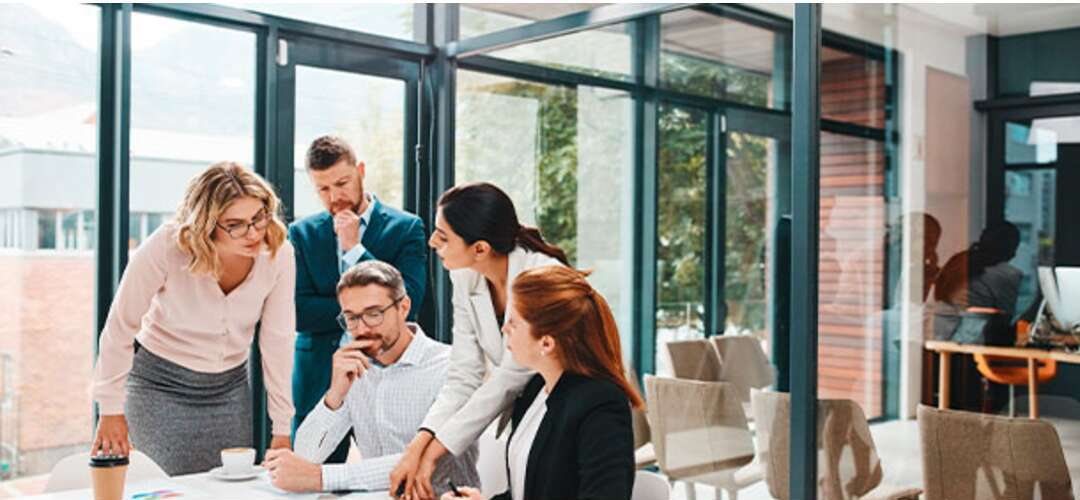
\includegraphics{images/passeio.jpg}
\caption{Produtor repassando software com os revisores}
\end{figure}

Existe uma revisão técnica formal chamada ``Passeio'' onde o \textbf{produtor} ``repassa'' o artefato de software, explicando o material, enquanto os \textbf{revisores} levantam questões com base em sua preparação prévia.

\subsubsection{B) Inspeção do produto}\label{b-inspeuxe7uxe3o-do-produto}

\begin{figure}
\centering

\includegraphics{images/inspecao.jpg}
\caption{Equipe fazendo inspeção constantemente no software}
\end{figure}

Na Inspeção do Produto de software, uma \textbf{pequena equipe} verifica o código sistematicamente, procurando por possíveis erros e omissões. Tudo é executado e controlado minuciosamente com \textbf{planilhas} e \textbf{documentos de formalização} assinados pelos gestores das áreas.

\subsubsection{C) Análise Estática}\label{c-anuxe1lise-estuxe1tica}

\begin{figure}
\centering
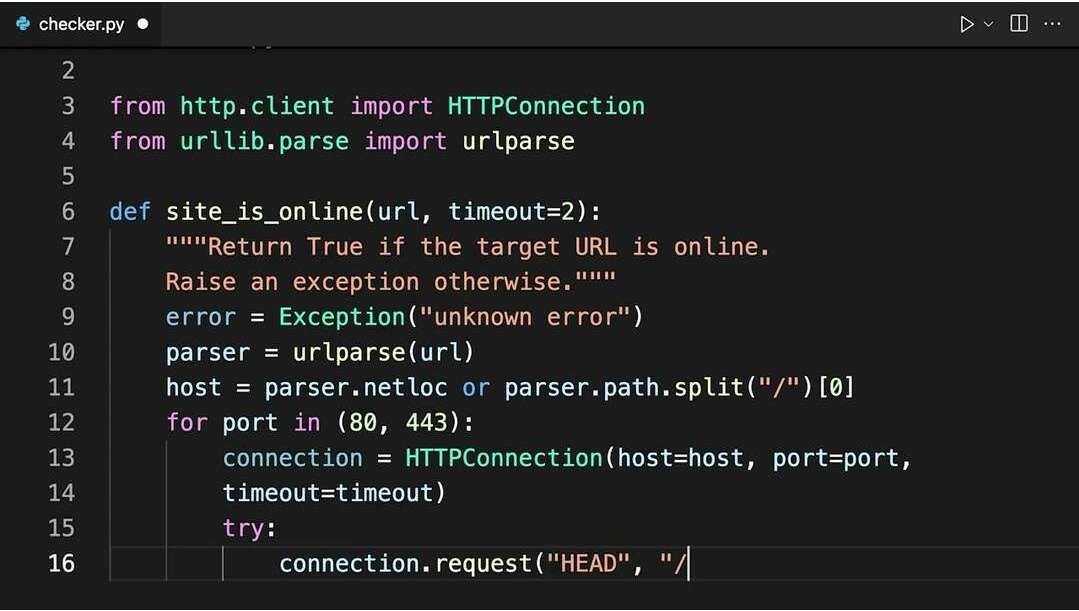
\includegraphics[width=3.875in,height=\textheight]{images/analise-estatica-python.jpg}
\caption{Código python revisado ``a olho''.}
\end{figure}

Inspeciona-se o código fonte do programa \textbf{sem executa-lo}, procurando erros de programação ``na raça''.

\subsubsection{D) Análise Estática Automatizada}\label{d-anuxe1lise-estuxe1tica-automatizada}

Inspeciona-se o código fonte do programa \textbf{com auxílio de um programa}, como por exemplo o \href{https://www.security-database.com/toolswatch/RATS-v2-3-Rough-Auditing-Tool-for.html}{RATS (Rough Auditing Tool for Security)} que significa ``Ferramenta de auditoria bruta para segurança''.

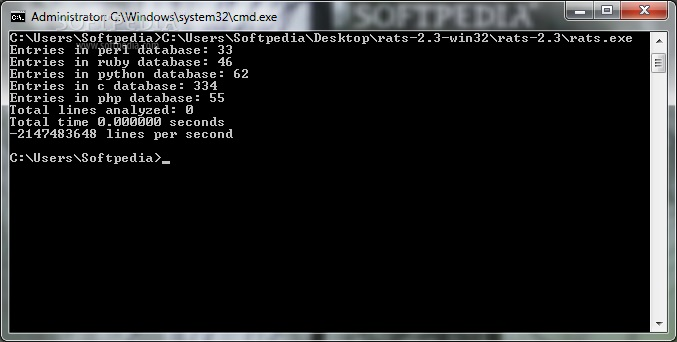
\includegraphics{images/VerificacaoValidacao/TecnicasEstaticas/rats-2.3.jpg}

\subsubsection{E) Verificação Formal do Produto e Métodos Formais}\label{e-verificauxe7uxe3o-formal-do-produto-e-muxe9todos-formais}

\begin{figure}
\centering
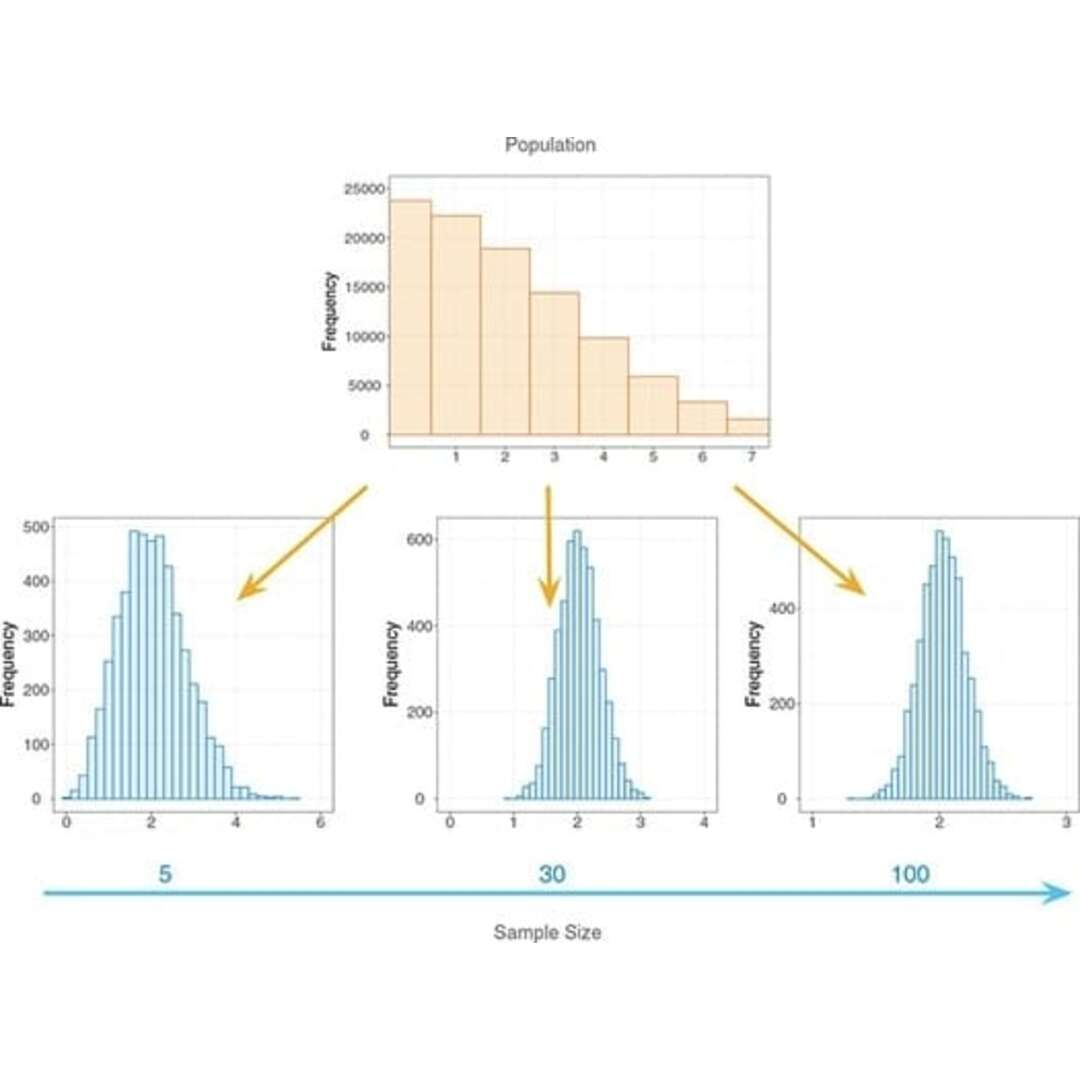
\includegraphics{images/estatistica.jpg}
\caption{Um teste de hipótese para validar software}
\end{figure}

Utiliza-se \textbf{métodos matemáticos e estatísticos} para avaliar o programa. Usado em software de missão crítica como software supervisório de usinas nucleares, cirurgia robótica e software de navegação de aviação.

\section{Verificação e Validação de software por Técnicas Dinâmicas}\label{verificauxe7uxe3o-e-validauxe7uxe3o-de-software-por-tuxe9cnicas-dinuxe2micas}

As Técnicas Dinâmicas são \textbf{testes de software}, nos quais o sistema é executado com dados de testes simulados.

\begin{longtable}[]{@{}
  >{\centering\arraybackslash}p{(\columnwidth - 2\tabcolsep) * \real{0.5000}}
  >{\raggedright\arraybackslash}p{(\columnwidth - 2\tabcolsep) * \real{0.5000}}@{}}
\toprule\noalign{}
\begin{minipage}[b]{\linewidth}\centering
Tipo de Teste
\end{minipage} & \begin{minipage}[b]{\linewidth}\raggedright
Descrição
\end{minipage} \\
\midrule\noalign{}
\endhead
\bottomrule\noalign{}
\endlastfoot
\ul{Teste de Unidade} & Concentra-se em \textbf{testar componentes individuais do software}, como módulos, classes ou funções, de forma isolada. O objetivo é verificar se cada unidade funciona corretamente em relação à sua especificação. Em um contexto orientado a objetos, isso inclui o teste de métodos dentro de uma classe. \\
\ul{Teste de Integração} & Após o teste de unidade, os \textbf{componentes são combinados e testados} em conjunto para \textbf{verificar as interações entre eles}. O teste de integração visa descobrir erros nas interfaces e na colaboração entre os módulos. \\
\ul{Teste de Validação} & Tem como objetivo \textbf{garantir que o software construído atende às expectativas e aos requisitos do cliente}. Os critérios de teste de validação são estabelecidos durante a análise de requisitos. \\
\ul{Teste de Sistema} & Testa o \textbf{software como um sistema completo}, após a integração de todos os componentes. \\
\end{longtable}

O teste de sistema pode ser separado em 6 subtestes:

\begin{longtable}[]{@{}
  >{\centering\arraybackslash}p{(\columnwidth - 2\tabcolsep) * \real{0.5000}}
  >{\raggedright\arraybackslash}p{(\columnwidth - 2\tabcolsep) * \real{0.5000}}@{}}
\toprule\noalign{}
\endhead
\bottomrule\noalign{}
\endlastfoot
\ul{Teste de Recuperação} & Verifica a capacidade do sistema de se \textbf{recuperar de falhas} (software ou hardware) e continuar operando corretamente. \\
\ul{Teste de Segurança} & Avalia se o sistema \textbf{protege dados e funcionalidades contra acessos não autorizados} e se cumpre os requisitos de privacidade e segurança. \\
\ul{Teste por Esforço} & Examina o comportamento do sistema sob \textbf{condições de carga anormal} (volume de dados, número de usuários, etc.) para identificar seus limites e possíveis pontos de falha. \\
\ul{Teste de Desempenho} & Avalia os \textbf{aspectos de desempenho do sistema}, como tempo de resposta, vazão e utilização de recursos, sob condições normais e de carga. \\
\ul{Teste de Disponibilização (Implantação/Configuração)} & Verifica se o software \textbf{opera corretamente em todos os ambientes} (plataformas, sistemas operacionais) para os quais foi projetado. Inclui também a avaliação dos procedimentos de instalação e da documentação associada. \\
\ul{Teste de Regressão} & É realizado após \textbf{alterações no software} (correção de erros, adição de novas funcionalidades) para garantir que as modificações não introduziram novos defeitos ou afetaram adversamente as partes existentes do sistema. \\
\end{longtable}

A escolha das técnicas dinâmicas e dos tipos de testes a serem utilizados depende do \textbf{tipo de software a ser desenvolvido}, dos \textbf{requisitos do projeto}, dos \textbf{recursos disponíveis} e dos \textbf{riscos envolvidos}. O objetivo final é \textbf{encontrar o maior número possível de erros} com o mínimo de esforço e garantir a entrega de software de alta qualidade que atenda às necessidades dos usuários.

\section{Exercícios}\label{exercuxedcios}

\subsection{Testes Sobre Verificação e Validação I}\label{testes-sobre-verificauxe7uxe3o-e-validauxe7uxe3o-i}

\begin{longtable}[]{@{}
  >{\raggedright\arraybackslash}p{(\columnwidth - 0\tabcolsep) * \real{1.0075}}@{}}
\toprule\noalign{}
\begin{minipage}[b]{\linewidth}\raggedright
\textbf{TESTE 1}
\end{minipage} \\
\midrule\noalign{}
\endhead
\bottomrule\noalign{}
\endlastfoot
Qual das seguintes afirmações melhor descreve o conceito de \textbf{verificação de software}? \\
\begin{minipage}[t]{\linewidth}\raggedright
\begin{enumerate}
\def\labelenumi{\Alph{enumi})}
\tightlist
\item
  É o processo de testar o software no ambiente do usuário final para garantir que ele atenda às suas necessidades e expectativas.
\end{enumerate}
\end{minipage} \\
\begin{minipage}[t]{\linewidth}\raggedright
\begin{enumerate}
\def\labelenumi{\Alph{enumi})}
\setcounter{enumi}{1}
\tightlist
\item
  Refere-se ao conjunto de atividades que visam descobrir erros e defeitos no software antes que ele seja entregue.
\end{enumerate}
\end{minipage} \\
\begin{minipage}[t]{\linewidth}\raggedright
\begin{enumerate}
\def\labelenumi{\Alph{enumi})}
\setcounter{enumi}{2}
\tightlist
\item
  Consiste em garantir que o software construído implementa corretamente as funcionalidades e requisitos especificados.
\end{enumerate}
\end{minipage} \\
\begin{minipage}[t]{\linewidth}\raggedright
\begin{enumerate}
\def\labelenumi{\Alph{enumi})}
\setcounter{enumi}{3}
\tightlist
\item
  Envolve a avaliação do desempenho do software em diferentes condições de carga e estresse para identificar gargalos.
\end{enumerate}
\end{minipage} \\
\begin{minipage}[t]{\linewidth}\raggedright
\begin{enumerate}
\def\labelenumi{\Alph{enumi})}
\setcounter{enumi}{4}
\tightlist
\item
  É a prática de gerenciar e controlar as mudanças feitas no software ao longo do seu ciclo de vida.
\end{enumerate}
\end{minipage} \\
\end{longtable}

\begin{longtable}[]{@{}
  >{\raggedright\arraybackslash}p{(\columnwidth - 0\tabcolsep) * \real{1.0062}}@{}}
\toprule\noalign{}
\begin{minipage}[b]{\linewidth}\raggedright
\textbf{TESTE 2}
\end{minipage} \\
\midrule\noalign{}
\endhead
\bottomrule\noalign{}
\endlastfoot
Qual das seguintes afirmações melhor descreve o conceito de \textbf{validação de software}? \\
\begin{minipage}[t]{\linewidth}\raggedright
\begin{enumerate}
\def\labelenumi{\Alph{enumi})}
\tightlist
\item
  É o processo de confirmar se o software está livre de defeitos através da execução de diversos casos de teste que cobrem o código em sua totalidade.
\end{enumerate}
\end{minipage} \\
\begin{minipage}[t]{\linewidth}\raggedright
\begin{enumerate}
\def\labelenumi{\Alph{enumi})}
\setcounter{enumi}{1}
\tightlist
\item
  Refere-se ao conjunto de atividades que garantem que o software foi construído corretamente, ou seja, em conformidade com as especificações de requisitos.
\end{enumerate}
\end{minipage} \\
\begin{minipage}[t]{\linewidth}\raggedright
\begin{enumerate}
\def\labelenumi{\Alph{enumi})}
\setcounter{enumi}{2}
\tightlist
\item
  Envolve a análise estática do código-fonte para identificar potenciais vulnerabilidades de segurança e garantir a conformidade com padrões de codificação.
\end{enumerate}
\end{minipage} \\
\begin{minipage}[t]{\linewidth}\raggedright
\begin{enumerate}
\def\labelenumi{\Alph{enumi})}
\setcounter{enumi}{3}
\tightlist
\item
  É a prática de documentar o design do software e garantir que a implementação esteja alinhada com a arquitetura definida.
\end{enumerate}
\end{minipage} \\
\begin{minipage}[t]{\linewidth}\raggedright
\begin{enumerate}
\def\labelenumi{\Alph{enumi})}
\setcounter{enumi}{4}
\tightlist
\item
  Consiste em avaliar se o software atende às necessidades e expectativas do cliente e dos usuários finais, assegurando que o ``produto certo'' foi construído.
\end{enumerate}
\end{minipage} \\
\end{longtable}

\begin{longtable}[]{@{}
  >{\raggedright\arraybackslash}p{(\columnwidth - 0\tabcolsep) * \real{1.0028}}@{}}
\toprule\noalign{}
\begin{minipage}[b]{\linewidth}\raggedright
\textbf{TESTE 3}
\end{minipage} \\
\midrule\noalign{}
\endhead
\bottomrule\noalign{}
\endlastfoot
Qual das seguintes afirmações descreve melhor a técnica de ``\textbf{Walkthrough}'' (passeio) no contexto de Verificação e Validação de software? \\
\begin{minipage}[t]{\linewidth}\raggedright
\begin{enumerate}
\def\labelenumi{\Alph{enumi})}
\tightlist
\item
  É uma técnica \textbf{dinâmica} que envolve a execução do software com dados de teste para observar seu comportamento e identificar defeitos em tempo de execução.
\end{enumerate}
\end{minipage} \\
\begin{minipage}[t]{\linewidth}\raggedright
\begin{enumerate}
\def\labelenumi{\Alph{enumi})}
\setcounter{enumi}{1}
\tightlist
\item
  Refere-se à aplicação de \textbf{métodos formais} que utilizam notação matemática para especificar e verificar as propriedades do software.
\end{enumerate}
\end{minipage} \\
\begin{minipage}[t]{\linewidth}\raggedright
\begin{enumerate}
\def\labelenumi{\Alph{enumi})}
\setcounter{enumi}{2}
\tightlist
\item
  Consiste na utilização de \textbf{testes automatizados} e ferramentas específicas para executar um grande número de casos de teste e verificar os resultados em relação às expectativas.
\end{enumerate}
\end{minipage} \\
\begin{minipage}[t]{\linewidth}\raggedright
\begin{enumerate}
\def\labelenumi{\Alph{enumi})}
\setcounter{enumi}{3}
\tightlist
\item
  Trata-se de uma \textbf{revisão técnica informal} ou \textbf{passeio informal} realizado com colegas, onde um produto de software (como um documento de requisitos, um projeto ou um trecho de código) é examinado passo a passo por um grupo para identificar possíveis erros, inconsistências, ou áreas que precisam de melhorias, \textbf{sem a execução do software}.
\end{enumerate}
\end{minipage} \\
\begin{minipage}[t]{\linewidth}\raggedright
\begin{enumerate}
\def\labelenumi{\Alph{enumi})}
\setcounter{enumi}{4}
\tightlist
\item
  Envolve a condução de \textbf{testes de aceitação pelo usuário} em um ambiente operacional para determinar se o software atende às necessidades do cliente e está pronto para ser implantado.
\end{enumerate}
\end{minipage} \\
\end{longtable}

\begin{longtable}[]{@{}
  >{\raggedright\arraybackslash}p{(\columnwidth - 0\tabcolsep) * \real{1.0076}}@{}}
\toprule\noalign{}
\begin{minipage}[b]{\linewidth}\raggedright
\textbf{TESTE 4}
\end{minipage} \\
\midrule\noalign{}
\endhead
\bottomrule\noalign{}
\endlastfoot
Qual das seguintes opções lista os tipos mais comuns de \textbf{técnicas estáticas} utilizadas em Verificação e Validação de software? \\
\begin{minipage}[t]{\linewidth}\raggedright
\begin{enumerate}
\def\labelenumi{\Alph{enumi})}
\tightlist
\item
  Revisões técnicas (incluindo inspeções e walkthroughs) e análise estática automatizada.
\end{enumerate}
\end{minipage} \\
\begin{minipage}[t]{\linewidth}\raggedright
\begin{enumerate}
\def\labelenumi{\Alph{enumi})}
\setcounter{enumi}{1}
\tightlist
\item
  Testes de unidade, testes de integração e testes de sistema.
\end{enumerate}
\end{minipage} \\
\begin{minipage}[t]{\linewidth}\raggedright
\begin{enumerate}
\def\labelenumi{\Alph{enumi})}
\setcounter{enumi}{2}
\tightlist
\item
  Testes alfa, testes beta e testes de aceitação pelo usuário.
\end{enumerate}
\end{minipage} \\
\begin{minipage}[t]{\linewidth}\raggedright
\begin{enumerate}
\def\labelenumi{\Alph{enumi})}
\setcounter{enumi}{3}
\tightlist
\item
  Testes de desempenho, testes de segurança e testes de carga.
\end{enumerate}
\end{minipage} \\
\begin{minipage}[t]{\linewidth}\raggedright
\begin{enumerate}
\def\labelenumi{\Alph{enumi})}
\setcounter{enumi}{4}
\tightlist
\item
  Depuração, teste de regressão e teste de fumaça.
\end{enumerate}
\end{minipage} \\
\end{longtable}

\begin{longtable}[]{@{}
  >{\raggedright\arraybackslash}p{(\columnwidth - 0\tabcolsep) * \real{1.0095}}@{}}
\toprule\noalign{}
\begin{minipage}[b]{\linewidth}\raggedright
TESTE 5
\end{minipage} \\
\midrule\noalign{}
\endhead
\bottomrule\noalign{}
\endlastfoot
Quem geralmente participa de uma inspeção formal de software (revisão técnica formal)? \\
\begin{minipage}[t]{\linewidth}\raggedright
\begin{enumerate}
\def\labelenumi{\Alph{enumi})}
\tightlist
\item
  Apenas os desenvolvedores responsáveis pela criação do artefato inspecionado.
\end{enumerate}
\end{minipage} \\
\begin{minipage}[t]{\linewidth}\raggedright
\begin{enumerate}
\def\labelenumi{\Alph{enumi})}
\setcounter{enumi}{1}
\tightlist
\item
  Uma equipe composta por diferentes papéis, como moderador, inspetor, relator e o autor do artefato.
\end{enumerate}
\end{minipage} \\
\begin{minipage}[t]{\linewidth}\raggedright
\begin{enumerate}
\def\labelenumi{\Alph{enumi})}
\setcounter{enumi}{2}
\tightlist
\item
  Somente os gerentes de projeto para avaliar o progresso e a conformidade com o cronograma.
\end{enumerate}
\end{minipage} \\
\begin{minipage}[t]{\linewidth}\raggedright
\begin{enumerate}
\def\labelenumi{\Alph{enumi})}
\setcounter{enumi}{3}
\tightlist
\item
  Exclusivamente os especialistas em testes para planejar os casos de teste futuros.
\end{enumerate}
\end{minipage} \\
\begin{minipage}[t]{\linewidth}\raggedright
\begin{enumerate}
\def\labelenumi{\Alph{enumi})}
\setcounter{enumi}{4}
\tightlist
\item
  Apenas o cliente para garantir que os requisitos foram atendidos.
\end{enumerate}
\end{minipage} \\
\end{longtable}

\begin{longtable}[]{@{}
  >{\raggedright\arraybackslash}p{(\columnwidth - 0\tabcolsep) * \real{1.0079}}@{}}
\toprule\noalign{}
\begin{minipage}[b]{\linewidth}\raggedright
TESTE 6
\end{minipage} \\
\midrule\noalign{}
\endhead
\bottomrule\noalign{}
\endlastfoot
Qual a principal característica que distingue a verificação formal de outras técnicas de verificação e validação de software? \\
\begin{minipage}[t]{\linewidth}\raggedright
\begin{enumerate}
\def\labelenumi{\Alph{enumi})}
\tightlist
\item
  A sua aplicação durante a fase de testes de unidade e integração.
\end{enumerate}
\end{minipage} \\
\begin{minipage}[t]{\linewidth}\raggedright
\begin{enumerate}
\def\labelenumi{\Alph{enumi})}
\setcounter{enumi}{1}
\tightlist
\item
  O uso de métodos matemáticos e lógicos para provar a correção do software em relação às suas especificações.
\end{enumerate}
\end{minipage} \\
\begin{minipage}[t]{\linewidth}\raggedright
\begin{enumerate}
\def\labelenumi{\Alph{enumi})}
\setcounter{enumi}{2}
\tightlist
\item
  A dependência da execução do software com dados de entrada reais.
\end{enumerate}
\end{minipage} \\
\begin{minipage}[t]{\linewidth}\raggedright
\begin{enumerate}
\def\labelenumi{\Alph{enumi})}
\setcounter{enumi}{3}
\tightlist
\item
  O foco na identificação de defeitos de usabilidade na interface do usuário.
\end{enumerate}
\end{minipage} \\
\begin{minipage}[t]{\linewidth}\raggedright
\begin{enumerate}
\def\labelenumi{\Alph{enumi})}
\setcounter{enumi}{4}
\tightlist
\item
  A sua realização por uma equipe de teste independente ao final do desenvolvimento.
\end{enumerate}
\end{minipage} \\
\end{longtable}

\begin{longtable}[]{@{}
  >{\raggedright\arraybackslash}p{(\columnwidth - 0\tabcolsep) * \real{1.0089}}@{}}
\toprule\noalign{}
\begin{minipage}[b]{\linewidth}\raggedright
TESTE 7
\end{minipage} \\
\midrule\noalign{}
\endhead
\bottomrule\noalign{}
\endlastfoot
Qual o principal objetivo da aplicação de métodos formais na verificação de um produto de software? \\
\begin{minipage}[t]{\linewidth}\raggedright
\begin{enumerate}
\def\labelenumi{\Alph{enumi})}
\tightlist
\item
  Melhorar a comunicação entre a equipe de desenvolvimento e os stakeholders.
\end{enumerate}
\end{minipage} \\
\begin{minipage}[t]{\linewidth}\raggedright
\begin{enumerate}
\def\labelenumi{\Alph{enumi})}
\setcounter{enumi}{1}
\tightlist
\item
  Garantir que o software seja portável para diferentes plataformas de hardware.
\end{enumerate}
\end{minipage} \\
\begin{minipage}[t]{\linewidth}\raggedright
\begin{enumerate}
\def\labelenumi{\Alph{enumi})}
\setcounter{enumi}{2}
\tightlist
\item
  Reduzir o tempo e o custo total do ciclo de vida do software.
\end{enumerate}
\end{minipage} \\
\begin{minipage}[t]{\linewidth}\raggedright
\begin{enumerate}
\def\labelenumi{\Alph{enumi})}
\setcounter{enumi}{3}
\tightlist
\item
  Aumentar o nível de confiança na correção do software, através de provas matemáticas de suas propriedades.
\end{enumerate}
\end{minipage} \\
\begin{minipage}[t]{\linewidth}\raggedright
\begin{enumerate}
\def\labelenumi{\Alph{enumi})}
\setcounter{enumi}{4}
\tightlist
\item
  Otimizar o desempenho do software em termos de velocidade e consumo de memória.
\end{enumerate}
\end{minipage} \\
\end{longtable}

\begin{longtable}[]{@{}
  >{\raggedright\arraybackslash}p{(\columnwidth - 0\tabcolsep) * \real{1.0081}}@{}}
\toprule\noalign{}
\begin{minipage}[b]{\linewidth}\raggedright
TESTE 8
\end{minipage} \\
\midrule\noalign{}
\endhead
\bottomrule\noalign{}
\endlastfoot
Qual das seguintes atividades é a principal característica das técnicas dinâmicas de verificação e validação de software? \\
\begin{minipage}[t]{\linewidth}\raggedright
\begin{enumerate}
\def\labelenumi{\Alph{enumi})}
\tightlist
\item
  A análise estática do código-fonte em busca de possíveis defeitos.
\end{enumerate}
\end{minipage} \\
\begin{minipage}[t]{\linewidth}\raggedright
\begin{enumerate}
\def\labelenumi{\Alph{enumi})}
\setcounter{enumi}{1}
\tightlist
\item
  A aplicação de métodos matemáticos para provar a correção do software.
\end{enumerate}
\end{minipage} \\
\begin{minipage}[t]{\linewidth}\raggedright
\begin{enumerate}
\def\labelenumi{\Alph{enumi})}
\setcounter{enumi}{2}
\tightlist
\item
  A revisão manual da documentação do software para garantir a sua completude.
\end{enumerate}
\end{minipage} \\
\begin{minipage}[t]{\linewidth}\raggedright
\begin{enumerate}
\def\labelenumi{\Alph{enumi})}
\setcounter{enumi}{3}
\tightlist
\item
  A execução do software com dados de entrada para observar seu comportamento e identificar erros.
\end{enumerate}
\end{minipage} \\
\begin{minipage}[t]{\linewidth}\raggedright
\begin{enumerate}
\def\labelenumi{\Alph{enumi})}
\setcounter{enumi}{4}
\tightlist
\item
  A inspeção formal dos artefatos de software por uma equipe multidisciplinar.
\end{enumerate}
\end{minipage} \\
\end{longtable}

\begin{longtable}[]{@{}
  >{\raggedright\arraybackslash}p{(\columnwidth - 0\tabcolsep) * \real{1.0076}}@{}}
\toprule\noalign{}
\begin{minipage}[b]{\linewidth}\raggedright
TESTE 9
\end{minipage} \\
\midrule\noalign{}
\endhead
\bottomrule\noalign{}
\endlastfoot
Qual o principal objetivo do teste de software como uma técnica dinâmica de verificação e validação? \\
\begin{minipage}[t]{\linewidth}\raggedright
\begin{enumerate}
\def\labelenumi{\Alph{enumi})}
\tightlist
\item
  Garantir que a documentação do software esteja completa e correta.
\end{enumerate}
\end{minipage} \\
\begin{minipage}[t]{\linewidth}\raggedright
\begin{enumerate}
\def\labelenumi{\Alph{enumi})}
\setcounter{enumi}{1}
\tightlist
\item
  Otimizar o desempenho do software em termos de velocidade e consumo de recursos.
\end{enumerate}
\end{minipage} \\
\begin{minipage}[t]{\linewidth}\raggedright
\begin{enumerate}
\def\labelenumi{\Alph{enumi})}
\setcounter{enumi}{2}
\tightlist
\item
  Encontrar erros no software, demonstrar que suas funções estão funcionando conforme as especificações e validar os requisitos.
\end{enumerate}
\end{minipage} \\
\begin{minipage}[t]{\linewidth}\raggedright
\begin{enumerate}
\def\labelenumi{\Alph{enumi})}
\setcounter{enumi}{3}
\tightlist
\item
  Verificar a conformidade do processo de desenvolvimento com os padrões estabelecidos.
\end{enumerate}
\end{minipage} \\
\begin{minipage}[t]{\linewidth}\raggedright
\begin{enumerate}
\def\labelenumi{\Alph{enumi})}
\setcounter{enumi}{4}
\tightlist
\item
  Avaliar a usabilidade da interface do usuário do software.
\end{enumerate}
\end{minipage} \\
\end{longtable}

\begin{longtable}[]{@{}
  >{\raggedright\arraybackslash}p{(\columnwidth - 0\tabcolsep) * \real{1.0063}}@{}}
\toprule\noalign{}
\begin{minipage}[b]{\linewidth}\raggedright
TESTE 10
\end{minipage} \\
\midrule\noalign{}
\endhead
\bottomrule\noalign{}
\endlastfoot
Qual dos seguintes níveis de teste é considerado uma técnica dinâmica de verificação e validação que foca em exercitar a menor unidade testável do software? \\
\begin{minipage}[t]{\linewidth}\raggedright
\begin{enumerate}
\def\labelenumi{\Alph{enumi})}
\tightlist
\item
  Teste de sistema.
\end{enumerate}
\end{minipage} \\
\begin{minipage}[t]{\linewidth}\raggedright
\begin{enumerate}
\def\labelenumi{\Alph{enumi})}
\setcounter{enumi}{1}
\tightlist
\item
  Teste de integração.
\end{enumerate}
\end{minipage} \\
\begin{minipage}[t]{\linewidth}\raggedright
\begin{enumerate}
\def\labelenumi{\Alph{enumi})}
\setcounter{enumi}{2}
\tightlist
\item
  Teste de validação.
\end{enumerate}
\end{minipage} \\
\begin{minipage}[t]{\linewidth}\raggedright
\begin{enumerate}
\def\labelenumi{\Alph{enumi})}
\setcounter{enumi}{3}
\tightlist
\item
  Teste de unidade.
\end{enumerate}
\end{minipage} \\
\begin{minipage}[t]{\linewidth}\raggedright
\begin{enumerate}
\def\labelenumi{\Alph{enumi})}
\setcounter{enumi}{4}
\tightlist
\item
  Teste de aceitação.
\end{enumerate}
\end{minipage} \\
\end{longtable}

\subsection{Respostas para os Testes}\label{respostas-para-os-testes}

\begin{longtable}[]{@{}ll@{}}
\toprule\noalign{}
Testes & Respostas \\
\midrule\noalign{}
\endhead
\bottomrule\noalign{}
\endlastfoot
Teste\_01 & C \\
Teste\_02 & E \\
Teste\_03 & D \\
Teste\_04 & A \\
Teste\_05 & B \\
Teste\_06 & B \\
Teste\_07 & D \\
Teste\_08 & D \\
Teste\_09 & C \\
Teste\_10 & D \\
\end{longtable}

\chapter{Verificação de Validação de Software II - Continuação}\label{verificauxe7uxe3o-de-validauxe7uxe3o-de-software-ii---continuauxe7uxe3o}

\section{Fundamentos de Teste de Software}\label{fundamentos-de-teste-de-software}

\textbf{O objetivo primordial do teste de software é descobrir erros}. Um bom teste é aquele que tem alta probabilidade de encontrar um erro. Como benefício secundário, os testes demonstram que as funções do software estão funcionando de acordo com as especificações e que os requisitos relativos ao desempenho e ao comportamento parecem estar sendo atingidos. Os dados coletados durante os testes fornecem um bom indício da confiabilidade e da qualidade geral do software. No entanto, é fundamental lembrar que \textbf{os testes não podem mostrar a ausência de erros e defeitos, apenas que erros e defeitos de software estão presentes}. Por isso, não se deve considerar o teste como uma ``rede de segurança'' que detectará todos os erros decorrentes de práticas deficientes de engenharia de software.

\section{Os testes e o Ciclo de Vida do Software}\label{os-testes-e-o-ciclo-de-vida-do-software}

\subsection{Teste de Unidade ou Unitários}\label{teste-de-unidade-ou-unituxe1rios}

Focado em testar cada componente individualmente para garantir que funcione adequadamente como uma unidade.

\paragraph{Ferramentas (bibliotecas) de teste unitário das linguagens de programação mais populares e robustas}\label{ferramentas-bibliotecas-de-teste-unituxe1rio-das-linguagens-de-programauxe7uxe3o-mais-populares-e-robustas}

\begin{longtable}[]{@{}
  >{\raggedright\arraybackslash}p{(\columnwidth - 4\tabcolsep) * \real{0.3333}}
  >{\raggedright\arraybackslash}p{(\columnwidth - 4\tabcolsep) * \real{0.3333}}
  >{\raggedright\arraybackslash}p{(\columnwidth - 4\tabcolsep) * \real{0.3333}}@{}}
\toprule\noalign{}
\begin{minipage}[b]{\linewidth}\raggedright
Nome do framework de teste de unidade
\end{minipage} & \begin{minipage}[b]{\linewidth}\raggedright
Linguagem
\end{minipage} & \begin{minipage}[b]{\linewidth}\raggedright
Logotipo
\end{minipage} \\
\midrule\noalign{}
\endhead
\bottomrule\noalign{}
\endlastfoot
Pytest & Python & 
\includegraphics[width=1.0625in,height=\textheight]{images/VerificacaoValidacao/TestesSoftware/pytest.jpg} \\
JUnit & Java & 
\includegraphics{images/VerificacaoValidacao/TestesSoftware/junit.jpg} \\
CTest & C++ & 
\includegraphics[width=0.95833in,height=\textheight]{images/VerificacaoValidacao/TestesSoftware/ctest.jpg} \\
\end{longtable}

\subsubsection{Exemplo de Teste Unitário no Python}\label{exemplo-de-teste-unituxe1rio-no-python}

Vamos testar uma função chamada \texttt{soma} que faça adição de dois números \texttt{a} e \texttt{b}.

Crie um arquivo \textbf{soma.py} que contém função chamada \texttt{soma} que faça adição de dois números \texttt{a} e \texttt{b} :

Código do arquivo soma segue abaixo:

\begin{Shaded}
\begin{Highlighting}[]

\CommentTok{\# arquivo soma.py}


\KeywordTok{def}\NormalTok{ soma(a, b):}
    \ControlFlowTok{return}\NormalTok{ a }\OperatorTok{+}\NormalTok{ b}
\end{Highlighting}
\end{Shaded}

Agora crie, no mesmo diretório, um arquivo cahamdo \textbf{test\_soma.py} .

Esse arquivo cria a função de este testa \texttt{test\_soma\_positivos()} que testa a função soma \texttt{soma} passando dois números \texttt{2} e \texttt{3} para ela.

O resultado esperado é 5 :

\begin{Shaded}
\begin{Highlighting}[]
\ImportTok{from}\NormalTok{ soma }\ImportTok{import}\NormalTok{ soma}

\KeywordTok{def}\NormalTok{ test\_soma\_positivos():}
    \ControlFlowTok{assert}\NormalTok{ soma(}\DecValTok{2}\NormalTok{, }\DecValTok{3}\NormalTok{) }\OperatorTok{==} \DecValTok{5}
    
\end{Highlighting}
\end{Shaded}

Então, estando os arquivos \textbf{soma.py} e \textbf{test\_soma.py} no mesmo arquivo, basta executar a ferramenta \textbf{pytest}

\begin{Shaded}
\begin{Highlighting}[]
\NormalTok{============================= test session starts ==============================}
\NormalTok{platform linux {-}{-} Python 3.x.x, pytest}\AttributeTok{{-}x}\NormalTok{.x.x, py}\AttributeTok{{-}x}\NormalTok{.x.x, pluggy}\AttributeTok{{-}x}\NormalTok{.x.x}
\NormalTok{rootdir: }\AttributeTok{/path/to/your/directory}

\NormalTok{collected 5 items}

\NormalTok{test\_soma.py .....                                                    [100\%]}

\NormalTok{============================== 5 passed in 0.01s ==============================}
\end{Highlighting}
\end{Shaded}

A função \textbf{soma()} passou no teste unitário.

\subsection{Teste de Integração}\label{teste-de-integrauxe7uxe3o}

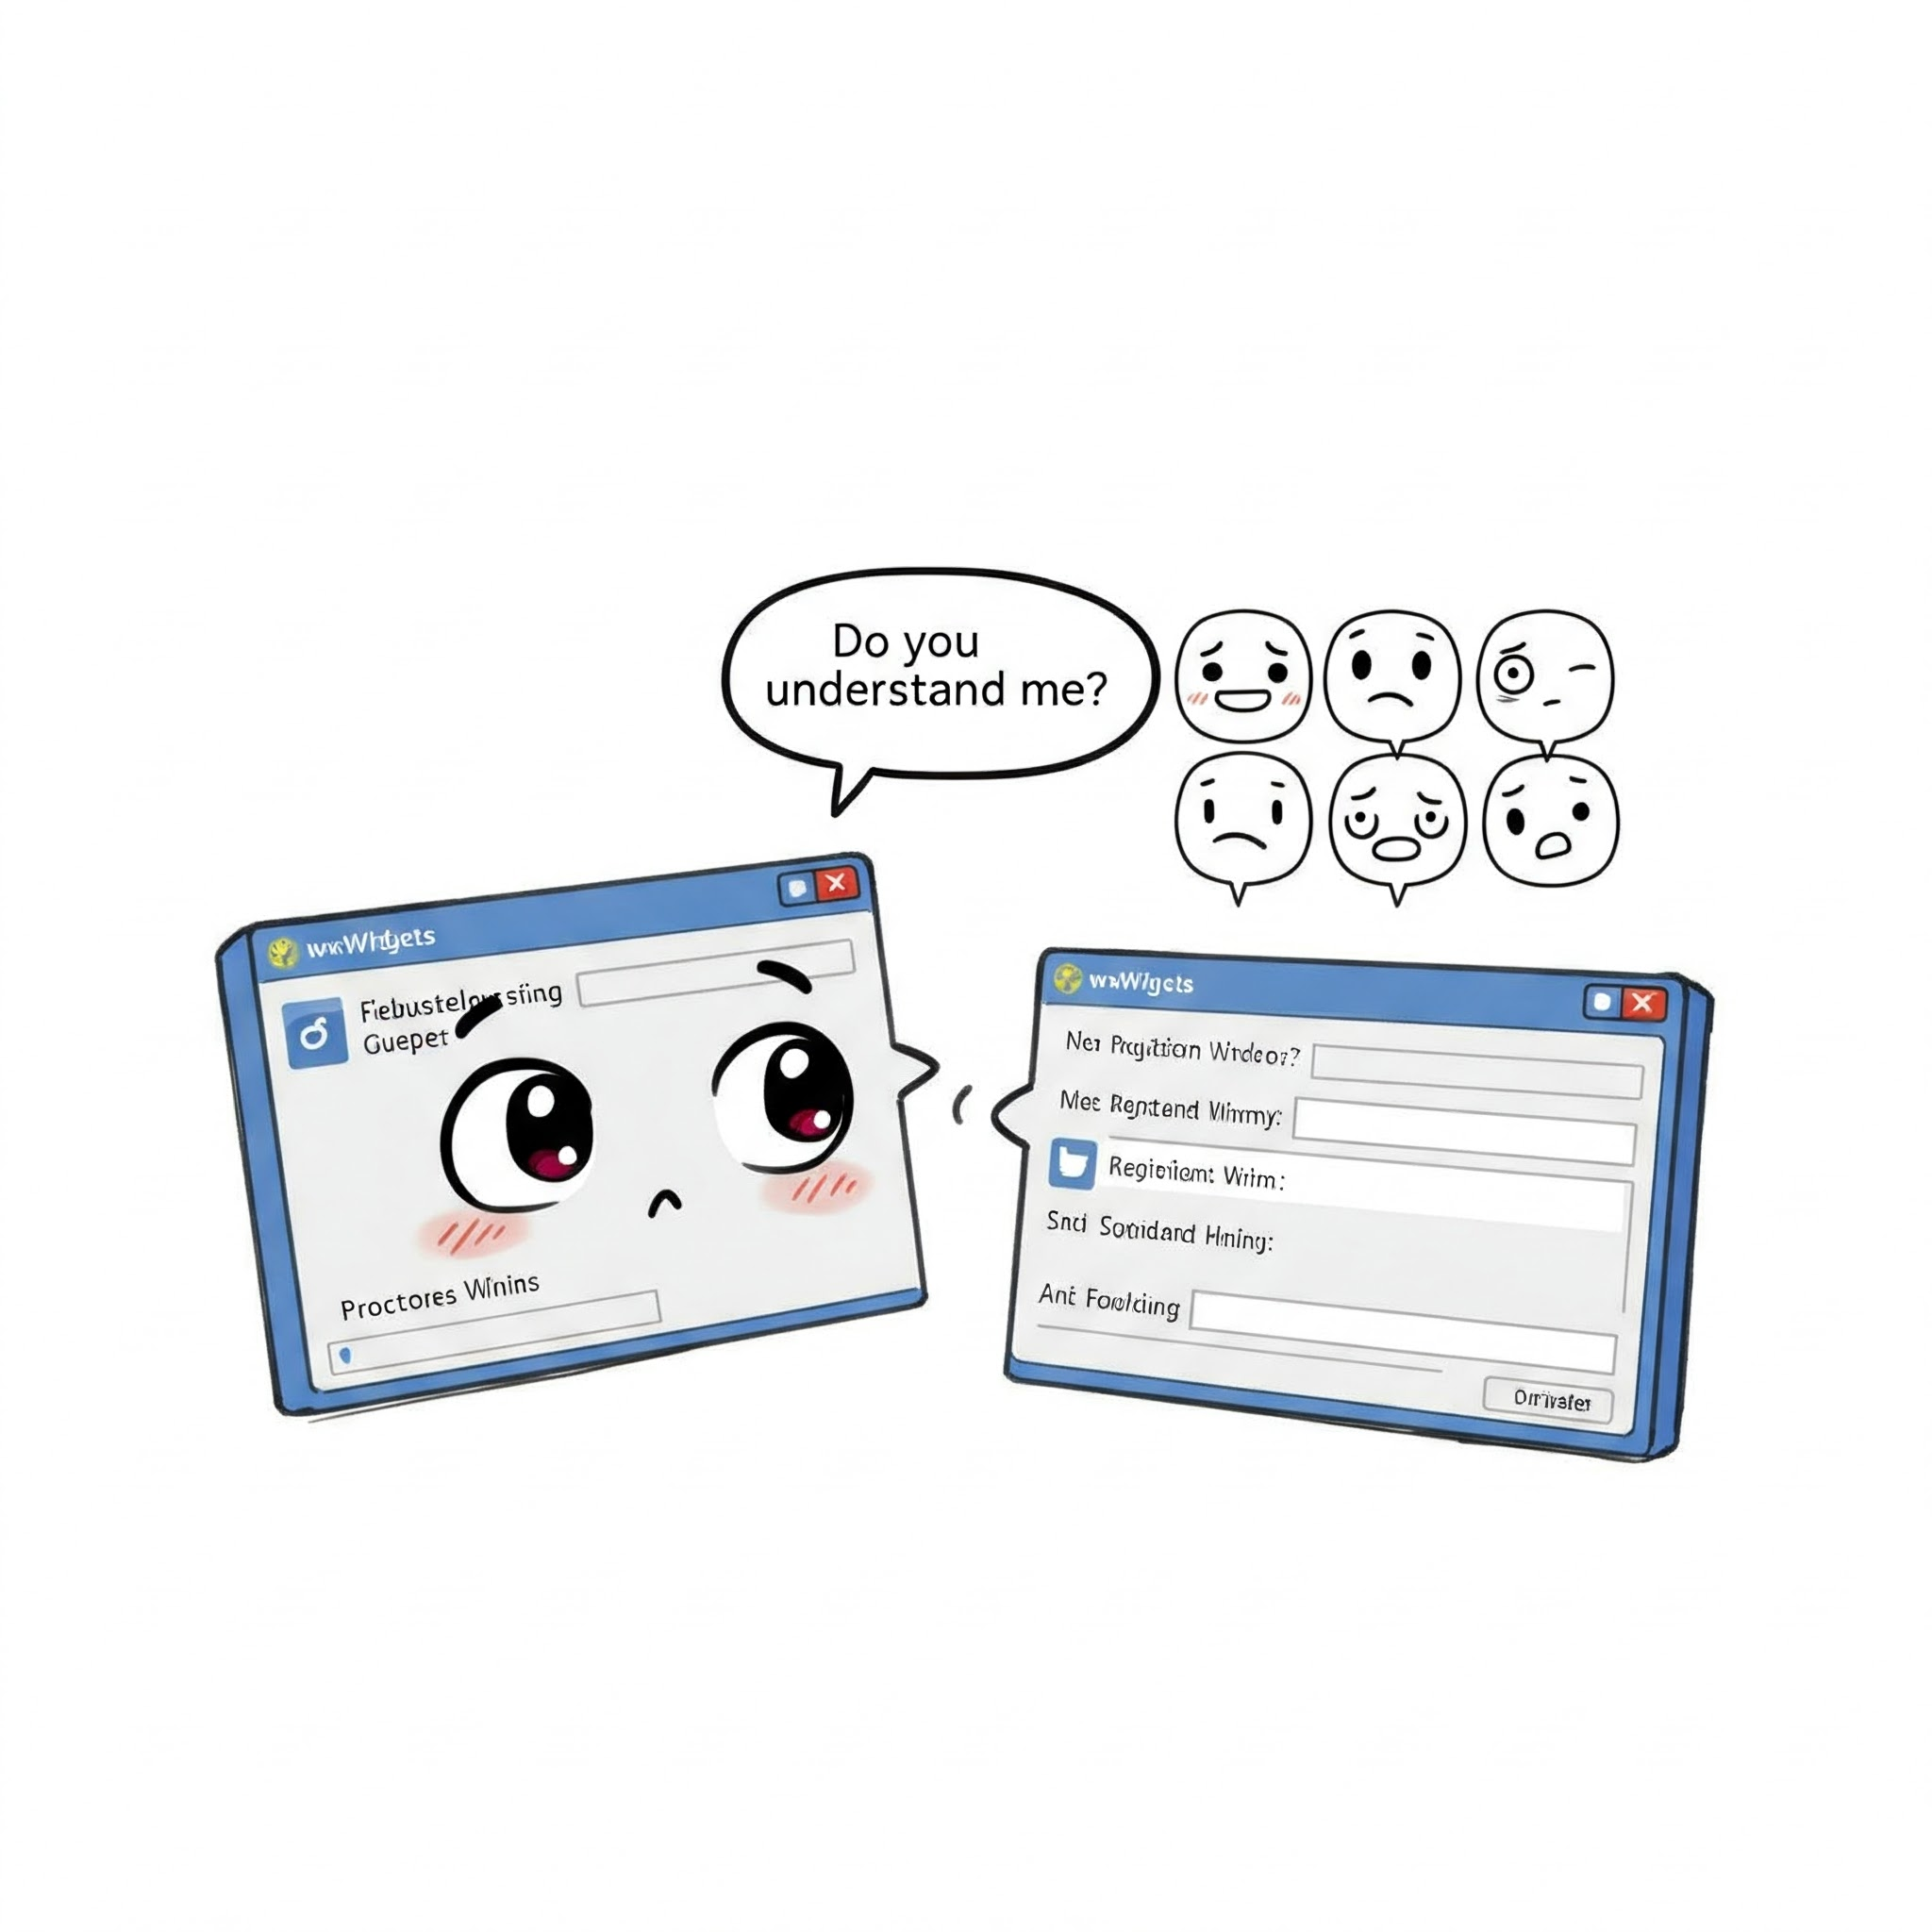
\includegraphics[width=3.60417in,height=\textheight]{images/VerificacaoValidacao/TestesSoftware/teste_integracao.jpeg}

Focado em testar cada componente individualmente para garantir que funcione adequadamente como uma unidade.

\subsection{Teste de Validação}\label{teste-de-validauxe7uxe3o}

Focado em testar cada componente individualmente para garantir que funcione adequadamente como uma unidade.

\subsection{Testes de Sistema}\label{testes-de-sistema}


\includegraphics[width=2.64583in,height=\textheight]{images/VerificacaoValidacao/TestesSoftware/teste_de_sistema.jpeg}

Focado em testar cada componente individualmente para garantir que funcione adequadamente como uma unidade.

\section{Modelo V}\label{modelo-v}


\includegraphics[width=2.02083in,height=\textheight]{images/VerificacaoValidacao/TestesSoftware/modelo_v.jpeg}

Em Testes de Software, o \textbf{Diagrama V (ou Modelo V)} é uma variação na representação do modelo cascata (ciclo de vida clássico) que descreve a relação entre \textbf{ações de garantia da qualidade (testes)} e as \textbf{ações associadas a comunicação, modelagem e atividades de construção iniciais}. Ele oferece uma maneira de \textbf{visualizar como as ações de verificação e validação são aplicadas a um trabalho de engenharia anterior}.

Em outras palavras, o modelo V correlaciona os \textbf{testes de Verificação e Validação de Software} ao \textbf{ciclo de Vida} do processo de desenvolvimento de Software \textbf{fornecendo a noção que o software é testado em todo seu ciclo de vida}:

\begin{longtable}[]{@{}
  >{\centering\arraybackslash}p{(\columnwidth - 2\tabcolsep) * \real{0.5373}}
  >{\centering\arraybackslash}p{(\columnwidth - 2\tabcolsep) * \real{0.4627}}@{}}
\toprule\noalign{}
\endhead
\bottomrule\noalign{}
\endlastfoot
\textbf{Etapa do Ciclo de Vida do Processo de Desenvolvimento de Software} & \textbf{Qualidade Testes de Verificação e Validação do Software} \\
\begin{minipage}[t]{\linewidth}\centering
\begin{itemize}
\tightlist
\item
  Elicitação de Requisitos
\end{itemize}
\end{minipage} & \begin{minipage}[t]{\linewidth}\centering
\begin{itemize}
\tightlist
\item
  Teste de aceitação
\end{itemize}
\end{minipage} \\
\begin{minipage}[t]{\linewidth}\centering
\begin{itemize}
\tightlist
\item
  Planejameno: Arquitetura do sistema
\end{itemize}
\end{minipage} & \begin{minipage}[t]{\linewidth}\centering
\begin{itemize}
\tightlist
\item
  Teste de Sistema
\end{itemize}
\end{minipage} \\
\begin{minipage}[t]{\linewidth}\centering
\begin{itemize}
\tightlist
\item
  Planejameno: Arquitetura dos Módulos
\end{itemize}
\end{minipage} & \begin{minipage}[t]{\linewidth}\centering
\begin{itemize}
\tightlist
\item
  Teste de Integração
\end{itemize}
\end{minipage} \\
\begin{minipage}[t]{\linewidth}\centering
\begin{itemize}
\tightlist
\item
  Codificação
\end{itemize}
\end{minipage} & \begin{minipage}[t]{\linewidth}\centering
\begin{itemize}
\tightlist
\item
  Teste Unitário
\end{itemize}
\end{minipage} \\
\end{longtable}

\begin{longtable}[]{@{}c@{}}
\toprule\noalign{}
\endhead
\bottomrule\noalign{}
\endlastfoot
\textbf{SOFTWARE PRONTO} \\
\end{longtable}

Esse correlacionamento pode ser visualizado na figura abaixo, em formato ``V'':

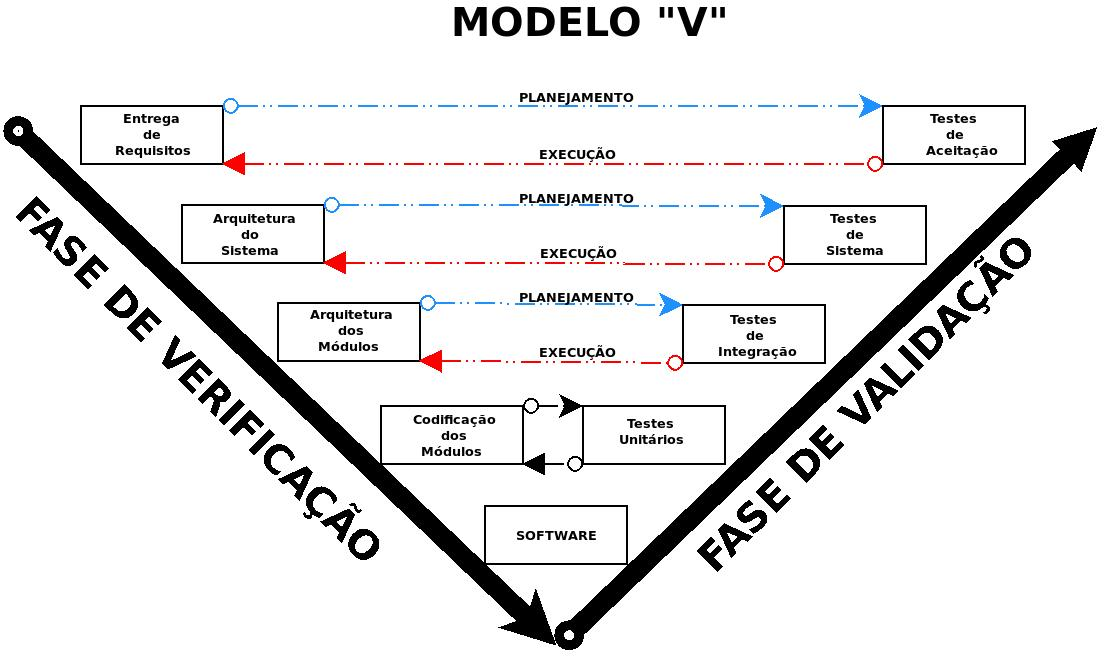
\includegraphics[width=8.33333in,height=\textheight]{images/VerificacaoValidacao/Modelo-V.jpg}

\section{Testes Unitários}\label{testes-unituxe1rios}

O objetivo primordial do teste unitário é \textbf{focar o esforço de verificação na menor unidade de projeto do software para descobrir erros dentro dos limites dessa unidade}. Ele busca garantir que cada parte individual do sistema funcione corretamente.

O teste unitário se concentra na \textbf{lógica interna de processamento e nas estruturas de dados dentro dos limites de um componente}. Ele examina os caminhos de controle importantes para descobrir erros na lógica do módulo.

\subsection{Testes Estruturais (Caixa-Branca)}\label{testes-estruturais-caixa-branca}


\includegraphics[width=3.16667in,height=\textheight]{images/VerificacaoValidacao/TestesSoftware/caixa_branca.jpeg}

Os t\textbf{estes caixa-branca}, também chamados de teste da caixa-de-vidro ou \textbf{teste estrutural}, são uma filosofia de projeto de casos de teste que utiliza a estrutura de controle descrita como parte do projeto no nível de componentes para derivar casos de teste.

O \textbf{teste de caixa-branca se alinha com o teste unitário}. O teste caixa-branca é frequentemente aplicado a \textbf{pequenos componentes de programas (por exemplo, módulos ou pequenos grupos de módulos)}, sendo considerado um ``teste no pequeno''.

\subsection{Testes Funcionais (Caixa-Preta)}\label{testes-funcionais-caixa-preta}


\includegraphics[width=4.125in,height=\textheight]{images/VerificacaoValidacao/TestesSoftware/caixa_preta.jpeg}

Os \textbf{testes caixa-preta}, também chamados de \textbf{teste comportamental} ou \textbf{teste funcional}, são uma abordagem de teste que \textbf{focaliza os requisitos funcionais do software}. Diferentemente dos testes caixa-branca, que examinam a estrutura lógica interna do software, o teste caixa-preta \textbf{faz referência a testes realizados na interface do software}, com \textbf{pouca preocupação em relação à estrutura lógica interna do software}. Em vez de olhar o código-fonte, os testadores caixa-preta trabalham com a \textbf{visão externa do software}.

\subsubsection{Técnicas de testes funcionais}\label{tuxe9cnicas-de-testes-funcionais}

\section{Exercícios}\label{exercuxedcios-1}

\subsection{Testes}\label{testes-1}

\begin{longtable}[]{@{}
  >{\raggedright\arraybackslash}p{(\columnwidth - 0\tabcolsep) * \real{1.0093}}@{}}
\toprule\noalign{}
\begin{minipage}[b]{\linewidth}\raggedright
TESTE 01
\end{minipage} \\
\midrule\noalign{}
\endhead
\bottomrule\noalign{}
\endlastfoot
Qual é o objetivo fundamental do Teste de Software ? \\
\begin{minipage}[t]{\linewidth}\raggedright
\begin{enumerate}
\def\labelenumi{\alph{enumi})}
\tightlist
\item
  Otimizar o desempenho do software para garantir uma melhor experiência do usuário.
\end{enumerate}
\end{minipage} \\
\begin{minipage}[t]{\linewidth}\raggedright
\begin{enumerate}
\def\labelenumi{\alph{enumi})}
\setcounter{enumi}{1}
\tightlist
\item
  Descobrir o maior número possível de erros e defeitos no software antes de sua entrega ou implantação.
\end{enumerate}
\end{minipage} \\
\begin{minipage}[t]{\linewidth}\raggedright
\begin{enumerate}
\def\labelenumi{\alph{enumi})}
\setcounter{enumi}{2}
\tightlist
\item
  Validar se o software está sendo desenvolvido dentro do prazo e do orçamento estipulados.
\end{enumerate}
\end{minipage} \\
\begin{minipage}[t]{\linewidth}\raggedright
\begin{enumerate}
\def\labelenumi{\alph{enumi})}
\setcounter{enumi}{3}
\tightlist
\item
  Garantir que o software seja compatível com todas as plataformas e dispositivos existentes.
\end{enumerate}
\end{minipage} \\
\begin{minipage}[t]{\linewidth}\raggedright
\begin{enumerate}
\def\labelenumi{\alph{enumi})}
\setcounter{enumi}{4}
\tightlist
\item
  Documentar detalhadamente todas as funcionalidades do software para referência futura.
\end{enumerate}
\end{minipage} \\
\end{longtable}

\begin{longtable}[]{@{}
  >{\raggedright\arraybackslash}p{(\columnwidth - 0\tabcolsep) * \real{1.0071}}@{}}
\toprule\noalign{}
\begin{minipage}[b]{\linewidth}\raggedright
TESTE 02
\end{minipage} \\
\midrule\noalign{}
\endhead
\bottomrule\noalign{}
\endlastfoot
No contexto de Testes de Software, qual a distinção essencial entre \textbf{verificação e validação}? \\
\begin{minipage}[t]{\linewidth}\raggedright
\begin{enumerate}
\def\labelenumi{\alph{enumi})}
\tightlist
\item
  Verificação foca em testar o software em diferentes ambientes, enquanto validação se concentra na sua funcionalidade.
\end{enumerate}
\end{minipage} \\
\begin{minipage}[t]{\linewidth}\raggedright
\begin{enumerate}
\def\labelenumi{\alph{enumi})}
\setcounter{enumi}{1}
\tightlist
\item
  Verificação é realizada pelos desenvolvedores, e validação é feita pelos usuários finais.
\end{enumerate}
\end{minipage} \\
\begin{minipage}[t]{\linewidth}\raggedright
\begin{enumerate}
\def\labelenumi{\alph{enumi})}
\setcounter{enumi}{2}
\tightlist
\item
  Verificação pergunta ``Estamos construindo o produto corretamente?'', enquanto validação pergunta ``Estamos construindo o produto certo?''
\end{enumerate}
\end{minipage} \\
\begin{minipage}[t]{\linewidth}\raggedright
\begin{enumerate}
\def\labelenumi{\alph{enumi})}
\setcounter{enumi}{3}
\tightlist
\item
  Validação ocorre antes da verificação no ciclo de vida de desenvolvimento de software.
\end{enumerate}
\end{minipage} \\
\begin{minipage}[t]{\linewidth}\raggedright
\begin{enumerate}
\def\labelenumi{\alph{enumi})}
\setcounter{enumi}{4}
\tightlist
\item
  Ambas se referem ao mesmo conjunto de atividades de garantia da qualidade.
\end{enumerate}
\end{minipage} \\
\end{longtable}

\begin{longtable}[]{@{}
  >{\raggedright\arraybackslash}p{(\columnwidth - 0\tabcolsep) * \real{1.0068}}@{}}
\toprule\noalign{}
\begin{minipage}[b]{\linewidth}\raggedright
TESTE 03
\end{minipage} \\
\midrule\noalign{}
\endhead
\bottomrule\noalign{}
\endlastfoot
Qual tipo de teste de software se baseia no \textbf{exame da estrutura interna} do software, incluindo seu código-fonte, para projetar casos de teste? \\
\begin{minipage}[t]{\linewidth}\raggedright
\begin{enumerate}
\def\labelenumi{\alph{enumi})}
\tightlist
\item
  Teste de caixa-preta
\end{enumerate}
\end{minipage} \\
\begin{minipage}[t]{\linewidth}\raggedright
\begin{enumerate}
\def\labelenumi{\alph{enumi})}
\setcounter{enumi}{1}
\tightlist
\item
  Teste de desempenho.
\end{enumerate}
\end{minipage} \\
\begin{minipage}[t]{\linewidth}\raggedright
\begin{enumerate}
\def\labelenumi{\alph{enumi})}
\setcounter{enumi}{2}
\tightlist
\item
  Teste de usabilidade.
\end{enumerate}
\end{minipage} \\
\begin{minipage}[t]{\linewidth}\raggedright
\begin{enumerate}
\def\labelenumi{\alph{enumi})}
\setcounter{enumi}{3}
\tightlist
\item
  Teste de caixa-branca (ou estrutural)
\end{enumerate}
\end{minipage} \\
\begin{minipage}[t]{\linewidth}\raggedright
\begin{enumerate}
\def\labelenumi{\alph{enumi})}
\setcounter{enumi}{4}
\tightlist
\item
  Teste de integração.
\end{enumerate}
\end{minipage} \\
\end{longtable}

\begin{longtable}[]{@{}
  >{\raggedright\arraybackslash}p{(\columnwidth - 0\tabcolsep) * \real{1.0098}}@{}}
\toprule\noalign{}
\begin{minipage}[b]{\linewidth}\raggedright
TESTE 4
\end{minipage} \\
\midrule\noalign{}
\endhead
\bottomrule\noalign{}
\endlastfoot
Por que é importante realizar testes em diferentes níveis (unidade, integração, validação, sistema)? \\
\begin{minipage}[t]{\linewidth}\raggedright
\begin{enumerate}
\def\labelenumi{\Alph{enumi})}
\tightlist
\item
  Para reduzir o custo total do processo de teste.
\end{enumerate}
\end{minipage} \\
\begin{minipage}[t]{\linewidth}\raggedright
\begin{enumerate}
\def\labelenumi{\Alph{enumi})}
\setcounter{enumi}{1}
\tightlist
\item
  Para facilitar a comunicação entre as equipes de desenvolvimento e teste.
\end{enumerate}
\end{minipage} \\
\begin{minipage}[t]{\linewidth}\raggedright
\begin{enumerate}
\def\labelenumi{\Alph{enumi})}
\setcounter{enumi}{2}
\tightlist
\item
  Porque diferentes tipos de erros são mais facilmente detectados em diferentes níveis de teste.
\end{enumerate}
\end{minipage} \\
\begin{minipage}[t]{\linewidth}\raggedright
\begin{enumerate}
\def\labelenumi{\Alph{enumi})}
\setcounter{enumi}{3}
\tightlist
\item
  Para garantir que todos os membros da equipe participem do processo de teste.
\end{enumerate}
\end{minipage} \\
\begin{minipage}[t]{\linewidth}\raggedright
\begin{enumerate}
\def\labelenumi{\Alph{enumi})}
\setcounter{enumi}{4}
\tightlist
\item
  Para cumprir as exigências de normas e padrões de qualidade como a ISO 9000.
\end{enumerate}
\end{minipage} \\
\end{longtable}

\begin{longtable}[]{@{}
  >{\raggedright\arraybackslash}p{(\columnwidth - 0\tabcolsep) * \real{1.0092}}@{}}
\toprule\noalign{}
\begin{minipage}[b]{\linewidth}\raggedright
TESTE 5
\end{minipage} \\
\midrule\noalign{}
\endhead
\bottomrule\noalign{}
\endlastfoot
Qual é a principal característica que o \textbf{Modelo V} busca explicitar em relação ao ciclo de vida clássico? \\
\begin{minipage}[t]{\linewidth}\raggedright
\begin{enumerate}
\def\labelenumi{\Alph{enumi})}
\tightlist
\item
  A natureza iterativa e incremental do desenvolvimento.
\end{enumerate}
\end{minipage} \\
\begin{minipage}[t]{\linewidth}\raggedright
\begin{enumerate}
\def\labelenumi{\Alph{enumi})}
\setcounter{enumi}{1}
\tightlist
\item
  A forte ênfase na comunicação com o cliente em todas as fases.
\end{enumerate}
\end{minipage} \\
\begin{minipage}[t]{\linewidth}\raggedright
\begin{enumerate}
\def\labelenumi{\Alph{enumi})}
\setcounter{enumi}{2}
\tightlist
\item
  O uso extensivo de prototipagem para validação precoce dos requisitos.
\end{enumerate}
\end{minipage} \\
\begin{minipage}[t]{\linewidth}\raggedright
\begin{enumerate}
\def\labelenumi{\Alph{enumi})}
\setcounter{enumi}{3}
\tightlist
\item
  A priorização da flexibilidade e adaptabilidade a mudanças nos requisitos.
\end{enumerate}
\end{minipage} \\
\begin{minipage}[t]{\linewidth}\raggedright
\begin{enumerate}
\def\labelenumi{\Alph{enumi})}
\setcounter{enumi}{4}
\tightlist
\item
  A relação entre as fases de desenvolvimento iniciais e as ações de garantia da qualidade (testes).
\end{enumerate}
\end{minipage} \\
\end{longtable}

\begin{longtable}[]{@{}
  >{\raggedright\arraybackslash}p{(\columnwidth - 0\tabcolsep) * \real{1.0081}}@{}}
\toprule\noalign{}
\begin{minipage}[b]{\linewidth}\raggedright
TESTE 6
\end{minipage} \\
\midrule\noalign{}
\endhead
\bottomrule\noalign{}
\endlastfoot
\textbf{Modelo V}, à medida que a equipe de software ``desce'' pelo lado esquerdo do ``V'', qual é o foco principal das atividades? \\
\begin{minipage}[t]{\linewidth}\raggedright
\begin{enumerate}
\def\labelenumi{\Alph{enumi})}
\tightlist
\item
  Implementação e codificação do sistema.
\end{enumerate}
\end{minipage} \\
\begin{minipage}[t]{\linewidth}\raggedright
\begin{enumerate}
\def\labelenumi{\Alph{enumi})}
\setcounter{enumi}{1}
\tightlist
\item
  Execução de testes unitários e de integração.
\end{enumerate}
\end{minipage} \\
\begin{minipage}[t]{\linewidth}\raggedright
\begin{enumerate}
\def\labelenumi{\Alph{enumi})}
\setcounter{enumi}{2}
\tightlist
\item
  Refinamento dos requisitos básicos em representações cada vez mais detalhadas do problema e da solução.
\end{enumerate}
\end{minipage} \\
\begin{minipage}[t]{\linewidth}\raggedright
\begin{enumerate}
\def\labelenumi{\Alph{enumi})}
\setcounter{enumi}{3}
\tightlist
\item
  Implantação e suporte contínuo do software.
\end{enumerate}
\end{minipage} \\
\begin{minipage}[t]{\linewidth}\raggedright
\begin{enumerate}
\def\labelenumi{\Alph{enumi})}
\setcounter{enumi}{4}
\tightlist
\item
  Gerenciamento do projeto e controle das mudanças.
\end{enumerate}
\end{minipage} \\
\end{longtable}

\begin{longtable}[]{@{}
  >{\raggedright\arraybackslash}p{(\columnwidth - 0\tabcolsep) * \real{1.0076}}@{}}
\toprule\noalign{}
\begin{minipage}[b]{\linewidth}\raggedright
TESTE 7
\end{minipage} \\
\midrule\noalign{}
\endhead
\bottomrule\noalign{}
\endlastfoot
No \textbf{Modelo V}, qual tipo de atividade de garantia da qualidade está tipicamente associada à fase de especificação de requisitos? \\
\begin{minipage}[t]{\linewidth}\raggedright
\begin{enumerate}
\def\labelenumi{\Alph{enumi})}
\tightlist
\item
  Teste de unidade.
\end{enumerate}
\end{minipage} \\
\begin{minipage}[t]{\linewidth}\raggedright
\begin{enumerate}
\def\labelenumi{\Alph{enumi})}
\setcounter{enumi}{1}
\tightlist
\item
  Teste de integração.
\end{enumerate}
\end{minipage} \\
\begin{minipage}[t]{\linewidth}\raggedright
\begin{enumerate}
\def\labelenumi{\Alph{enumi})}
\setcounter{enumi}{2}
\tightlist
\item
  Teste de sistema.
\end{enumerate}
\end{minipage} \\
\begin{minipage}[t]{\linewidth}\raggedright
\begin{enumerate}
\def\labelenumi{\Alph{enumi})}
\setcounter{enumi}{3}
\tightlist
\item
  Teste de aceitação (validação dos requisitos).
\end{enumerate}
\end{minipage} \\
\begin{minipage}[t]{\linewidth}\raggedright
\begin{enumerate}
\def\labelenumi{\Alph{enumi})}
\setcounter{enumi}{4}
\tightlist
\item
  Teste de desempenho.
\end{enumerate}
\end{minipage} \\
\end{longtable}

\begin{longtable}[]{@{}
  >{\raggedright\arraybackslash}p{(\columnwidth - 0\tabcolsep) * \real{1.0100}}@{}}
\toprule\noalign{}
\begin{minipage}[b]{\linewidth}\raggedright
TESTE 8
\end{minipage} \\
\midrule\noalign{}
\endhead
\bottomrule\noalign{}
\endlastfoot
Segundo o \textbf{Modelo V}, as atividades de teste no lado direito do ``V'' têm como objetivo principal: \\
\begin{minipage}[t]{\linewidth}\raggedright
\begin{enumerate}
\def\labelenumi{\Alph{enumi})}
\tightlist
\item
  Otimizar o desempenho do software.
\end{enumerate}
\end{minipage} \\
\begin{minipage}[t]{\linewidth}\raggedright
\begin{enumerate}
\def\labelenumi{\Alph{enumi})}
\setcounter{enumi}{1}
\tightlist
\item
  Validar cada um dos modelos criados à medida que a equipe ``desceu'' pelo lado esquerdo.
\end{enumerate}
\end{minipage} \\
\begin{minipage}[t]{\linewidth}\raggedright
\begin{enumerate}
\def\labelenumi{\Alph{enumi})}
\setcounter{enumi}{2}
\tightlist
\item
  Garantir a segurança do sistema contra ameaças.
\end{enumerate}
\end{minipage} \\
\begin{minipage}[t]{\linewidth}\raggedright
\begin{enumerate}
\def\labelenumi{\Alph{enumi})}
\setcounter{enumi}{3}
\tightlist
\item
  Documentar o código-fonte de forma detalhada.
\end{enumerate}
\end{minipage} \\
\begin{minipage}[t]{\linewidth}\raggedright
\begin{enumerate}
\def\labelenumi{\Alph{enumi})}
\setcounter{enumi}{4}
\tightlist
\item
  Facilitar a manutenção futura do software.
\end{enumerate}
\end{minipage} \\
\end{longtable}

\begin{longtable}[]{@{}
  >{\raggedright\arraybackslash}p{(\columnwidth - 0\tabcolsep) * \real{1.0095}}@{}}
\toprule\noalign{}
\begin{minipage}[b]{\linewidth}\raggedright
TESTE 9
\end{minipage} \\
\midrule\noalign{}
\endhead
\bottomrule\noalign{}
\endlastfoot
No \textbf{Modelo V}, o teste de sistema, que está ligado à fase de projeto da arquitetura do sistema, visa: \\
\begin{minipage}[t]{\linewidth}\raggedright
\begin{enumerate}
\def\labelenumi{\Alph{enumi})}
\tightlist
\item
  Testar as interações entre os componentes.
\end{enumerate}
\end{minipage} \\
\begin{minipage}[t]{\linewidth}\raggedright
\begin{enumerate}
\def\labelenumi{\Alph{enumi})}
\setcounter{enumi}{1}
\tightlist
\item
  Avaliar a facilidade de manutenção do código.
\end{enumerate}
\end{minipage} \\
\begin{minipage}[t]{\linewidth}\raggedright
\begin{enumerate}
\def\labelenumi{\Alph{enumi})}
\setcounter{enumi}{2}
\tightlist
\item
  Validar os requisitos do cliente em um ambiente de produção.
\end{enumerate}
\end{minipage} \\
\begin{minipage}[t]{\linewidth}\raggedright
\begin{enumerate}
\def\labelenumi{\Alph{enumi})}
\setcounter{enumi}{3}
\tightlist
\item
  Garantir que cada unidade de código funcione corretamente.
\end{enumerate}
\end{minipage} \\
\begin{minipage}[t]{\linewidth}\raggedright
\begin{enumerate}
\def\labelenumi{\Alph{enumi})}
\setcounter{enumi}{4}
\tightlist
\item
  Verificar se o software integrado funciona conforme o especificado nos requisitos do sistema.
\end{enumerate}
\end{minipage} \\
\end{longtable}

\begin{longtable}[]{@{}
  >{\raggedright\arraybackslash}p{(\columnwidth - 0\tabcolsep) * \real{1.0079}}@{}}
\toprule\noalign{}
\begin{minipage}[b]{\linewidth}\raggedright
TESTE 10
\end{minipage} \\
\midrule\noalign{}
\endhead
\bottomrule\noalign{}
\endlastfoot
Qual a principal vantagem de visualizar o processo de teste através do \textbf{Modelo V}? \\
\begin{minipage}[t]{\linewidth}\raggedright
\begin{enumerate}
\def\labelenumi{\Alph{enumi})}
\tightlist
\item
  Facilita a adoção de metodologias ágeis.
\end{enumerate}
\end{minipage} \\
\begin{minipage}[t]{\linewidth}\raggedright
\begin{enumerate}
\def\labelenumi{\Alph{enumi})}
\setcounter{enumi}{1}
\tightlist
\item
  Reduz a necessidade de documentação detalhada.
\end{enumerate}
\end{minipage} \\
\begin{minipage}[t]{\linewidth}\raggedright
\begin{enumerate}
\def\labelenumi{\Alph{enumi})}
\setcounter{enumi}{2}
\tightlist
\item
  Oferece uma maneira clara de como as ações de verificação e validação se relacionam com as atividades de desenvolvimento.
\end{enumerate}
\end{minipage} \\
\begin{minipage}[t]{\linewidth}\raggedright
\begin{enumerate}
\def\labelenumi{\Alph{enumi})}
\setcounter{enumi}{3}
\tightlist
\item
  Garante a automação completa de todos os testes.
\end{enumerate}
\end{minipage} \\
\begin{minipage}[t]{\linewidth}\raggedright
\begin{enumerate}
\def\labelenumi{\Alph{enumi})}
\setcounter{enumi}{4}
\tightlist
\item
  Elimina a necessidade de revisões técnicas.
\end{enumerate}
\end{minipage} \\
\end{longtable}

\subsection{Respostas dos Testes}\label{respostas-dos-testes}

\begin{longtable}[]{@{}ll@{}}
\toprule\noalign{}
Teste & Resposta \\
\midrule\noalign{}
\endhead
\bottomrule\noalign{}
\endlastfoot
\textbf{Teste\_01} & B \\
\textbf{Teste\_02} & C \\
\textbf{Teste\_03} & D \\
\textbf{Teste\_04} & C \\
\textbf{Teste\_05} & E \\
\textbf{Teste\_06} & C \\
\textbf{Teste\_07} & D \\
\textbf{Teste\_08} & B \\
\textbf{Teste\_09} & E \\
\textbf{Teste\_10} & C \\
\end{longtable}

\subsection{Questões Dissertativas:}\label{questuxf5es-dissertativas}

\begin{longtable}[]{@{}
  >{\raggedright\arraybackslash}p{(\columnwidth - 0\tabcolsep) * \real{1.0000}}@{}}
\toprule\noalign{}
\endhead
\bottomrule\noalign{}
\endlastfoot
\textbf{Questão 1} \\
Discuta a \textbf{importância da distinção entre verificação e validação} no contexto de testes de software. Explique como cada uma dessas atividades contribui para a garantia da qualidade do produto final, citando as definições apresentadas nas fontes. \\
\end{longtable}

\textbf{Resposta:} \_\_\_\_\_\_\_\_\_\_\_\_\_\_\_\_\_\_\_\_\_\_\_\_\_\_\_\_\_\_\_\_\_\_\_\_\_\_\_\_\_\_\_\_\_\_\_\_\_\_\_\_\_\_\_\_\_\_\_\_\_\_\_\_\_\_\_\_\_\_\_\_\_\_\_\_\_\_\_\_\_\_\_\_\_\_\_\_\_\_\_\_\_\_\_\_\_\_\_\_\_\_\_\_\_\_\_\_\_\_\_\_\_\_\_\_\_\_\_\_\_\_\_\_\_\_\_\_\_\_\_\_\_\_\_\_\_\_\_\_\_\_\_\_\_\_\_\_\_\_\_\_\_\_\_\_\_\_\_\_\_\_\_\_\_\_\_\_\_\_\_\_\_\_\_\_\_\_\_\_\_\_\_\_\_\_\_\_\_\_\_\_\_\_\_\_\_\_\_\_\_\_\_\_\_\_\_\_\_\_\_\_\_\_\_\_\_\_\_\_\_\_\_\_\_\_\_\_\_\_\_\_\_\_\_\_\_\_\_\_\_\_\_\_\_\_\_\_\_\_\_\_\_\_\_\_\_\_\_\_\_\_\_\_\_\_\_\_\_\_\_\_\_\_\_\_\_\_\_\_\_\_\_\_\_\_\_\_\_\_\_\_\_\_\_\_\_\_\_\_\_\_\_\_\_\_\_\_\_\_\_\_\_\_\_\_\_\_\_\_\_\_\_\_\_\_\_\_\_\_\_\_\_\_\_\_\_\_\_\_\_\_\_\_\_\_\_\_\_\_\_\_\_\_\_\_\_\_\_\_\_\_\_\_\_\_\_\_\_\_\_\_\_\_\_\_\_\_\_\_\_\_\_\_\_\_\_\_\_\_\_\_\_\_\_\_\_\_\_\_\_\_\_\_\_\_\_\_\_\_\_\_\_\_\_\_\_\_\_\_\_\_\_\_\_\_\_\_\_\_\_\_\_\_\_\_\_\_\_\_\_\_\_\_\_\_\_\_\_\_\_\_\_\_\_\_\_\_\_\_\_\_\_\_\_\_\_\_\_\_\_\_\_\_\_\_\_\_\_\_\_\_\_\_\_\_\_\_\_\_\_\_\_\_\_\_\_\_\_\_\_\_\_\_\_\_\_\_\_\_\_\_\_\_\_\_\_\_\_\_\_\_\_\_\_\_\_\_\_\_\_\_\_\_\_\_\_\_\_\_\_\_\_\_\_\_\_\_\_\_\_\_\_\_\_\_\_\_\_\_\_\_\_\_\_\_\_\_\_\_\_\_\_\_\_\_\_\_\_\_\_\_\_\_\_\_\_\_\_\_\_\_\_\_\_\_\_\_\_\_\_\_\_\_\_\_\_\_\_\_\_\_\_\_\_\_\_\_\_\_\_\_\_\_\_\_\_\_\_\_\_\_\_\_\_\_\_\_\_\_\_\_\_\_\_\_\_\_\_\_\_\_\_\_\_\_\_\_\_\_\_\_\_\_\_\_\_\_\_\_\_\_\_\_\_\_\_\_\_\_\_\_\_\_\_\_\_\_\_\_\_\_\_\_\_\_\_\_\_\_\_\_\_\_\_\_\_\_\_\_\_\_\_\_\_\_\_\_\_\_\_\_\_\_\_\_\_\_\_\_\_\_\_\_\_\_\_\_\_\_\_\_\_\_\_\_\_\_\_\_\_\_\_\_\_\_\_\_\_\_\_\_\_\_\_\_\_\_\_\_\_\_\_\_\_\_\_\_\_\_\_\_\_\_\_\_\_\_\_\_\_\_\_\_\_\_\_\_\_\_\_\_\_\_\_\_\_\_\_\_\_\_\_\_\_\_\_\_\_\_\_\_\_\_\_\_\_\_\_\_\_\_\_\_\_\_\_\_\_\_\_\_\_\_\_\_\_\_\_\_\_\_\_\_\_\_\_\_\_\_\_\_\_\_\_\_\_\_\_\_\_\_\_\_\_\_\_\_\_\_\_\_\_\_\_\_\_\_\_\_\_\_\_\_\_\_\_\_\_\_\_\_\_\_\_\_\_\_\_\_\_\_\_\_\_\_\_\_\_\_\_\_\_\_\_\_\_\_\_\_\_\_\_\_\_\_\_\_\_\_\_\_\_\_\_\_\_\_\_\_\_\_\_\_\_\_\_\_\_\_\_\_\_\_\_\_\_\_\_\_\_\_\_\_\_\_\_\_\_\_\_\_\_\_\_\_\_\_\_\_\_\_\_\_\_\_\_\_\_\_\_\_\_\_\_\_\_\_\_\_\_\_\_\_\_\_\_\_\_\_\_\_\_\_\_\_\_\_\_\_\_\_\_\_\_\_\_\_\_\_\_\_\_\_\_\_\_\_\_\_\_\_\_\_\_\_\_\_\_\_\_\_\_\_\_\_\_\_\_\_\_\_\_\_\_\_\_\_\_\_\_\_\_\_\_\_\_\_\_\_\_\_\_\_\_\_\_\_\_\_\_\_\_\_\_\_\_\_\_\_\_\_\_\_\_\_\_\_\_\_\_\_\_\_\_\_\_\_\_\_\_\_\_\_\_\_\_\_\_\_\_\_\_\_\_\_\_\_\_\_\_\_\_\_\_\_\_\_\_\_\_\_\_\_\_\_\_\_\_\_\_\_\_\_\_\_\_\_\_\_\_\_\_\_\_\_\_\_\_\_\_\_\_\_\_\_\_\_\_\_\_\_\_\_\_\_\_\_\_\_\_\_\_\_\_\_\_\_\_\_\_\_\_\_\_\_\_\_\_\_\_\_\_\_\_\_\_\_\_\_\_\_\_\_\_\_\_\_\_\_\_\_\_\_\_\_\_\_\_\_\_\_\_\_\_\_\_\_\_\_\_\_\_\_\_\_\_\_\_\_\_\_\_\_\_\_\_\_\_\_\_\_\_\_\_\_\_\_\_\_\_\_\_\_\_\_\_\_\_\_\_\_\_\_\_\_\_\_\_\_\_\_\_\_\_\_\_\_\_\_\_\_\_\_\_\_\_\_\_\_\_\_\_\_\_\_\_\_\_\_\_\_\_\_\_\_\_\_\_\_\_\_\_\_\_\_\_\_\_\_\_\_\_\_\_\_\_\_\_\_\_\_\_\_\_\_\_\_\_\_\_\_\_\_\_\_\_\_\_\_\_\_\_\_\_\_\_\_\_\_\_\_\_\_\_\_\_\_\_\_\_\_\_\_\_\_\_\_\_\_\_\_\_\_\_\_\_\_\_\_\_\_\_\_\_\_\_\_\_\_\_\_\_\_\_\_\_\_\_\_\_\_\_\_\_\_\_\_\_\_\_\_\_\_\_\_\_\_\_\_\_\_\_\_\_\_\_\_\_\_\_\_\_\_\_\_\_\_\_\_\_\_\_\_\_\_\_\_\_\_\_\_\_\_\_\_\_\_\_\_\_\_\_\_\_\_\_\_\_\_\_\_\_\_\_\_\_\_\_\_\_\_\_\_\_\_\_\_\_\_\_\_\_\_\_\_\_\_\_\_\_\_\_\_\_\_\_\_

\begin{longtable}[]{@{}
  >{\raggedright\arraybackslash}p{(\columnwidth - 0\tabcolsep) * \real{1.0000}}@{}}
\toprule\noalign{}
\endhead
\bottomrule\noalign{}
\endlastfoot
\textbf{Questão 2} \\
Compare e contraste as abordagens de teste de \textbf{caixa-branca} e \textbf{caixa-preta}. Para cada abordagem, descreva seus focos principais, as informações necessárias para sua aplicação. Avalie as vantagens e desvantagens de cada uma na detecção de diferentes tipos de defeitos. \\
\end{longtable}

\textbf{Resposta:} \_\_\_\_\_\_\_\_\_\_\_\_\_\_\_\_\_\_\_\_\_\_\_\_\_\_\_\_\_\_\_\_\_\_\_\_\_\_\_\_\_\_\_\_\_\_\_\_\_\_\_\_\_\_\_\_\_\_\_\_\_\_\_\_\_\_\_\_\_\_\_\_\_\_\_\_\_\_\_\_\_\_\_\_\_\_\_\_\_\_\_\_\_\_\_\_\_\_\_\_\_\_\_\_\_\_\_\_\_\_\_\_\_\_\_\_\_\_\_\_\_\_\_\_\_\_\_\_\_\_\_\_\_\_\_\_\_\_\_\_\_\_\_\_\_\_\_\_\_\_\_\_\_\_\_\_\_\_\_\_\_\_\_\_\_\_\_\_\_\_\_\_\_\_\_\_\_\_\_\_\_\_\_\_\_\_\_\_\_\_\_\_\_\_\_\_\_\_\_\_\_\_\_\_\_\_\_\_\_\_\_\_\_\_\_\_\_\_\_\_\_\_\_\_\_\_\_\_\_\_\_\_\_\_\_\_\_\_\_\_\_\_\_\_\_\_\_\_\_\_\_\_\_\_\_\_\_\_\_\_\_\_\_\_\_\_\_\_\_\_\_\_\_\_\_\_\_\_\_\_\_\_\_\_\_\_\_\_\_\_\_\_\_\_\_\_\_\_\_\_\_\_\_\_\_\_\_\_\_\_\_\_\_\_\_\_\_\_\_\_\_\_\_\_\_\_\_\_\_\_\_\_\_\_\_\_\_\_\_\_\_\_\_\_\_\_\_\_\_\_\_\_\_\_\_\_\_\_\_\_\_\_\_\_\_\_\_\_\_\_\_\_\_\_\_\_\_\_\_\_\_\_\_\_\_\_\_\_\_\_\_\_\_\_\_\_\_\_\_\_\_\_\_\_\_\_\_\_\_\_\_\_\_\_\_\_\_\_\_\_\_\_\_\_\_\_\_\_\_\_\_\_\_\_\_\_\_\_\_\_\_\_\_\_\_\_\_\_\_\_\_\_\_\_\_\_\_\_\_\_\_\_\_\_\_\_\_\_\_\_\_\_\_\_\_\_\_\_\_\_\_\_\_\_\_\_\_\_\_\_\_\_\_\_\_\_\_\_\_\_\_\_\_\_\_\_\_\_\_\_\_\_\_\_\_\_\_\_\_\_\_\_\_\_\_\_\_\_\_\_\_\_\_\_\_\_\_\_\_\_\_\_\_\_\_\_\_\_\_\_\_\_\_\_\_\_\_\_\_\_\_\_\_\_\_\_\_\_\_\_\_\_\_\_\_\_\_\_\_\_\_\_\_\_\_\_\_\_\_\_\_\_\_\_\_\_\_\_\_\_\_\_\_\_\_\_\_\_\_\_\_\_\_\_\_\_\_\_\_\_\_\_\_\_\_\_\_\_\_\_\_\_\_\_\_\_\_\_\_\_\_\_\_\_\_\_\_\_\_\_\_\_\_\_\_\_\_\_\_\_\_\_\_\_\_\_\_\_\_\_\_\_\_\_\_\_\_\_\_\_\_\_\_\_\_\_\_\_\_\_\_\_\_\_\_\_\_\_\_\_\_\_\_\_\_\_\_\_\_\_\_\_\_\_\_\_\_\_\_\_\_\_\_\_\_\_\_\_\_\_\_\_\_\_\_\_\_\_\_\_\_\_\_\_\_\_\_\_\_\_\_\_\_\_\_\_\_\_\_\_\_\_\_\_\_\_\_\_\_\_\_\_\_\_\_\_\_\_\_\_\_\_\_\_\_\_\_\_\_\_\_\_\_\_\_\_\_\_\_\_\_\_\_\_\_\_\_\_\_\_\_\_\_\_\_\_\_\_\_\_\_\_\_\_\_\_\_\_\_\_\_\_\_\_\_\_\_\_\_\_\_\_\_\_\_\_\_\_\_\_\_\_\_\_\_\_\_\_\_\_\_\_\_\_\_\_\_\_\_\_\_\_\_\_\_\_\_\_\_\_\_\_\_\_\_\_\_\_\_\_\_\_\_\_\_\_\_\_\_\_\_\_\_\_\_\_\_\_\_\_\_\_\_\_\_\_\_\_\_\_\_\_\_\_\_\_\_\_\_\_\_\_\_\_\_\_\_\_\_\_\_\_\_\_\_\_\_\_\_\_\_\_\_\_\_\_\_\_\_\_\_\_\_\_\_\_\_\_\_\_\_\_\_\_\_\_\_\_\_\_\_\_\_\_\_\_\_\_\_\_\_\_\_\_\_\_\_\_\_\_\_\_\_\_\_\_\_\_\_\_\_\_\_\_\_\_\_\_\_\_\_\_\_\_\_\_\_\_\_\_\_\_\_\_\_\_\_\_\_\_\_\_\_\_\_\_\_\_\_\_\_\_\_\_\_\_\_\_\_\_\_\_\_\_\_\_\_\_\_\_\_\_\_\_\_\_\_\_\_\_\_\_\_\_\_\_\_\_\_\_\_\_\_\_\_\_\_\_\_\_\_\_\_\_\_\_\_\_\_\_\_\_\_\_\_\_\_\_\_\_\_\_\_\_\_\_\_\_\_\_\_\_\_\_\_\_\_\_\_\_\_\_\_\_\_\_\_\_\_\_\_\_\_\_\_\_\_\_\_\_\_\_\_\_\_\_\_\_\_\_\_\_\_\_\_\_\_\_\_\_\_\_\_\_\_\_\_\_\_\_\_\_\_\_\_\_\_\_\_\_\_\_\_\_\_\_\_\_\_\_\_\_\_\_\_\_\_\_\_\_\_\_\_\_\_\_\_\_\_\_\_\_\_\_\_\_\_\_\_\_\_\_\_\_\_\_\_\_\_\_\_\_\_\_\_\_\_\_\_\_\_\_\_\_\_\_\_\_\_\_\_\_\_\_\_\_\_\_\_\_\_\_\_\_\_\_\_\_\_\_\_\_\_\_\_\_\_\_\_\_\_\_\_\_\_\_\_\_\_\_\_\_\_\_\_\_\_\_\_\_\_\_\_\_\_\_\_\_\_\_\_\_\_\_\_\_\_\_\_\_\_\_\_\_\_\_\_\_\_\_\_\_\_\_\_\_\_\_\_\_\_\_\_\_\_\_\_\_\_\_\_\_\_\_\_\_\_\_\_\_\_\_\_\_\_\_\_\_\_\_\_\_\_\_\_\_\_\_\_\_\_\_\_\_\_\_\_\_\_\_\_\_\_\_\_\_\_\_\_\_\_\_\_\_\_\_\_\_\_\_\_\_\_\_\_\_\_\_\_\_\_\_\_\_\_\_\_\_\_\_\_\_\_\_\_\_\_\_\_\_\_\_\_\_\_\_\_\_\_\_\_\_\_\_\_\_\_\_\_\_\_\_\_\_\_\_\_\_\_\_\_\_\_\_\_\_\_\_\_\_\_\_\_\_\_\_\_\_\_\_\_\_\_\_\_\_\_\_\_\_\_\_\_\_\_\_\_\_\_\_\_\_\_\_\_\_\_\_\_\_\_\_\_\_\_\_\_\_\_\_\_\_\_\_\_\_\_\_\_\_\_\_\_\_\_\_\_\_

\begin{longtable}[]{@{}
  >{\raggedright\arraybackslash}p{(\columnwidth - 0\tabcolsep) * \real{1.0000}}@{}}
\toprule\noalign{}
\endhead
\bottomrule\noalign{}
\endlastfoot
\textbf{Questão 3} \\
Explore a \textbf{relação entre os diferentes níveis de teste} (unidade, integração, validação e sistema) no ciclo de vida do software. Explique os objetivos específicos de cada nível e como eles se complementam para garantir a qualidade em diferentes granularidades do sistema. \\
\end{longtable}

\textbf{Resposta:} \_\_\_\_\_\_\_\_\_\_\_\_\_\_\_\_\_\_\_\_\_\_\_\_\_\_\_\_\_\_\_\_\_\_\_\_\_\_\_\_\_\_\_\_\_\_\_\_\_\_\_\_\_\_\_\_\_\_\_\_\_\_\_\_\_\_\_\_\_\_\_\_\_\_\_\_\_\_\_\_\_\_\_\_\_\_\_\_\_\_\_\_\_\_\_\_\_\_\_\_\_\_\_\_\_\_\_\_\_\_\_\_\_\_\_\_\_\_\_\_\_\_\_\_\_\_\_\_\_\_\_\_\_\_\_\_\_\_\_\_\_\_\_\_\_\_\_\_\_\_\_\_\_\_\_\_\_\_\_\_\_\_\_\_\_\_\_\_\_\_\_\_\_\_\_\_\_\_\_\_\_\_\_\_\_\_\_\_\_\_\_\_\_\_\_\_\_\_\_\_\_\_\_\_\_\_\_\_\_\_\_\_\_\_\_\_\_\_\_\_\_\_\_\_\_\_\_\_\_\_\_\_\_\_\_\_\_\_\_\_\_\_\_\_\_\_\_\_\_\_\_\_\_\_\_\_\_\_\_\_\_\_\_\_\_\_\_\_\_\_\_\_\_\_\_\_\_\_\_\_\_\_\_\_\_\_\_\_\_\_\_\_\_\_\_\_\_\_\_\_\_\_\_\_\_\_\_\_\_\_\_\_\_\_\_\_\_\_\_\_\_\_\_\_\_\_\_\_\_\_\_\_\_\_\_\_\_\_\_\_\_\_\_\_\_\_\_\_\_\_\_\_\_\_\_\_\_\_\_\_\_\_\_\_\_\_\_\_\_\_\_\_\_\_\_\_\_\_\_\_\_\_\_\_\_\_\_\_\_\_\_\_\_\_\_\_\_\_\_\_\_\_\_\_\_\_\_\_\_\_\_\_\_\_\_\_\_\_\_\_\_\_\_\_\_\_\_\_\_\_\_\_\_\_\_\_\_\_\_\_\_\_\_\_\_\_\_\_\_\_\_\_\_\_\_\_\_\_\_\_\_\_\_\_\_\_\_\_\_\_\_\_\_\_\_\_\_\_\_\_\_\_\_\_\_\_\_\_\_\_\_\_\_\_\_\_\_\_\_\_\_\_\_\_\_\_\_\_\_\_\_\_\_\_\_\_\_\_\_\_\_\_\_\_\_\_\_\_\_\_\_\_\_\_\_\_\_\_\_\_\_\_\_\_\_\_\_\_\_\_\_\_\_\_\_\_\_\_\_\_\_\_\_\_\_\_\_\_\_\_\_\_\_\_\_\_\_\_\_\_\_\_\_\_\_\_\_\_\_\_\_\_\_\_\_\_\_\_\_\_\_\_\_\_\_\_\_\_\_\_\_\_\_\_\_\_\_\_\_\_\_\_\_\_\_\_\_\_\_\_\_\_\_\_\_\_\_\_\_\_\_\_\_\_\_\_\_\_\_\_\_\_\_\_\_\_\_\_\_\_\_\_\_\_\_\_\_\_\_\_\_\_\_\_\_\_\_\_\_\_\_\_\_\_\_\_\_\_\_\_\_\_\_\_\_\_\_\_\_\_\_\_\_\_\_\_\_\_\_\_\_\_\_\_\_\_\_\_\_\_\_\_\_\_\_\_\_\_\_\_\_\_\_\_\_\_\_\_\_\_\_\_\_\_\_\_\_\_\_\_\_\_\_\_\_\_\_\_\_\_\_\_\_\_\_\_\_\_\_\_\_\_\_\_\_\_\_\_\_\_\_\_\_\_\_\_\_\_\_\_\_\_\_\_\_\_\_\_\_\_\_\_\_\_\_\_\_\_\_\_\_\_\_\_\_\_\_\_\_\_\_\_\_\_\_\_\_\_\_\_\_\_\_\_\_\_\_\_\_\_\_\_\_\_\_\_\_\_\_\_\_\_\_\_\_\_\_\_\_\_\_\_\_\_\_\_\_\_\_\_\_\_\_\_\_\_\_\_\_\_\_\_\_\_\_\_\_\_\_\_\_\_\_\_\_\_\_\_\_\_\_\_\_\_\_\_\_\_\_\_\_\_\_\_\_\_\_\_\_\_\_\_\_\_\_\_\_\_\_\_\_\_\_\_\_\_\_\_\_\_\_\_\_\_\_\_\_\_\_\_\_\_\_\_\_\_\_\_\_\_\_\_\_\_\_\_\_\_\_\_\_\_\_\_\_\_\_\_\_\_\_\_\_\_\_\_\_\_\_\_\_\_\_\_\_\_\_\_\_\_\_\_\_\_\_\_\_\_\_\_\_\_\_\_\_\_\_\_\_\_\_\_\_\_\_\_\_\_\_\_\_\_\_\_\_\_\_\_\_\_\_\_\_\_\_\_\_\_\_\_\_\_\_\_\_\_\_\_\_\_\_\_\_\_\_\_\_\_\_\_\_\_\_\_\_\_\_\_\_\_\_\_\_\_\_\_\_\_\_\_\_\_\_\_\_\_\_\_\_\_\_\_\_\_\_\_\_\_\_\_\_\_\_\_\_\_\_\_\_\_\_\_\_\_\_\_\_\_\_\_\_\_\_\_\_\_\_\_\_\_\_\_\_\_\_\_\_\_\_\_\_\_\_\_\_\_\_\_\_\_\_\_\_\_\_\_\_\_\_\_\_\_\_\_\_\_\_\_\_\_\_\_\_\_\_\_\_\_\_\_\_\_\_\_\_\_\_\_\_\_\_\_\_\_\_\_\_\_\_\_\_\_\_\_\_\_\_\_\_\_\_\_\_\_\_\_\_\_\_\_\_\_\_\_\_\_\_\_\_\_\_\_\_\_\_\_\_\_\_\_\_\_\_\_\_\_\_\_\_\_\_\_\_\_\_\_\_\_\_\_\_\_\_\_\_\_\_\_\_\_\_\_\_\_\_\_\_\_\_\_\_\_\_\_\_\_\_\_\_\_\_\_\_\_\_\_\_\_\_\_\_\_\_\_\_\_\_\_\_\_\_\_\_\_\_\_\_\_\_\_\_\_\_\_\_\_\_\_\_\_\_\_\_\_\_\_\_\_\_\_\_\_\_\_\_\_\_\_\_\_\_\_\_\_\_\_\_\_\_\_\_\_\_\_\_\_\_\_\_\_\_\_\_\_\_\_\_\_\_\_\_\_\_\_\_\_\_\_\_\_\_\_\_\_\_\_\_\_\_\_\_\_\_\_\_\_\_\_\_\_\_\_\_\_\_\_\_\_\_\_\_\_\_\_\_\_\_\_\_\_\_\_\_\_\_\_\_\_\_\_\_\_\_\_\_\_\_\_\_\_\_\_\_\_\_\_\_\_\_\_\_\_\_\_\_\_\_\_\_\_\_\_\_\_\_\_\_\_\_\_\_\_\_\_\_\_\_\_\_\_\_\_\_\_\_\_\_\_\_\_\_\_\_\_\_\_\_\_\_\_\_\_\_\_\_\_\_\_\_\_\_\_\_\_\_\_\_\_\_\_\_\_\_\_\_\_\_\_\_\_\_\_\_\_\_\_\_\_\_\_\_\_\_\_\_\_\_\_

\subsection{Respostas Questões Dissertativas:}\label{respostas-questuxf5es-dissertativas}

\begin{longtable}[]{@{}
  >{\raggedright\arraybackslash}p{(\columnwidth - 0\tabcolsep) * \real{1.0024}}@{}}
\toprule\noalign{}
\endhead
\bottomrule\noalign{}
\endlastfoot
\textbf{Resposta questão 1} \\
A distinção entre \textbf{verificação} e \textbf{validação} é fundamental em testes de software para garantir a qualidade sob diferentes perspectivas.

\textbf{Verificação} busca responder à pergunta: ``\textbf{Estamos criando o produto corretamente?}''. Envolve um conjunto de tarefas que asseguram que o software foi construído e pode ser rastreado segundo os requisitos do cliente. Isso inclui diversas atividades de garantia da qualidade de software (SQA), como revisões técnicas, auditorias de qualidade e configuração, monitoramento de desempenho e revisão de documentação.

Por outro lado, a \textbf{validação} procura responder: ``\textbf{Estamos criando o produto certo?}''. Ela se refere a um conjunto de tarefas que asseguram que o software criado atende às reais necessidades dos usuários. A validação de software é alcançada por meio de uma série de testes que demonstram conformidade com os requisitos.

Um plano de teste descreve as classes de testes a serem realizados para garantir que todos os requisitos funcionais, características comportamentais, conteúdo, requisitos de desempenho e documentação estejam corretos.

Ambas as atividades são cruciais: a verificação garante que o software está sendo construído de acordo com as especificações, enquanto a validação assegura que as especificações atendem às necessidades do cliente, contribuindo assim para um produto final de alta qualidade. \\
\end{longtable}

\begin{longtable}[]{@{}
  >{\raggedright\arraybackslash}p{(\columnwidth - 0\tabcolsep) * \real{1.0015}}@{}}
\toprule\noalign{}
\endhead
\bottomrule\noalign{}
\endlastfoot
\textbf{Resposta questão 2} \\
As abordagens de teste de software podem ser amplamente categorizadas em \textbf{caixa-branca} (ou \emph{white-box}) e \textbf{caixa-preta} (ou \emph{black-box}). O \textbf{teste caixa-branca} foca na \textbf{estrutura interna do software}, incluindo sua lógica, código e fluxo de controle. Para aplicar testes de caixa-branca, é necessário \textbf{conhecimento detalhado do código-fonte} e do design do software. A vantagem do teste caixa-branca é sua capacidade de \textbf{descobrir erros lógicos internos}, caminhos não percorridos e problemas na implementação. No entanto, pode ser \textbf{difícil e demorado} para sistemas complexos e não detecta necessariamente erros relacionados aos requisitos ou à usabilidade.

Em contraste, o \textbf{teste caixa-preta} examina a \textbf{funcionalidade do software} do ponto de vista do usuário, \textbf{sem conhecimento de sua implementação interna}. As informações necessárias são os \textbf{requisitos do software}, as especificações e a interface do usuário. A principal vantagem do teste caixa-preta é sua capacidade de \textbf{validar os requisitos do software} e identificar problemas na funcionalidade e usabilidade percebidas pelo usuário. Sua desvantagem é que ele \textbf{não garante a cobertura de toda a lógica interna} do software e pode não detectar certos tipos de erros de implementação.

Ambas as abordagens são importantes e complementares para garantir uma qualidade abrangente do software. \\
\end{longtable}

\begin{longtable}[]{@{}
  >{\raggedright\arraybackslash}p{(\columnwidth - 0\tabcolsep) * \real{1.0021}}@{}}
\toprule\noalign{}
\endhead
\bottomrule\noalign{}
\endlastfoot
\textbf{Resposta questão 3} \\
A estratégia de teste de software geralmente envolve múltiplos níveis que abordam a qualidade em diferentes granularidades do sistema.

O \textbf{teste de unidade} é o primeiro nível e se concentra em \textbf{testar individualmente cada unidade} (componente, classe ou função) do software, conforme implementado no código-fonte. O objetivo é \textbf{verificar a funcionalidade básica e a correção} de cada parte isoladamente.

Após as unidades serem testadas, o próximo nível é o \textbf{teste de integração}, que se concentra em \textbf{testar as interfaces e a interação entre os diferentes componentes} que foram integrados para construir a arquitetura do software. O objetivo é \textbf{descobrir erros nas interfaces entre módulos} e os efeitos colaterais causados pela adição de novas unidades.

O \textbf{teste de sistema} avalia o \textbf{software integrado como um todo}, juntamente com outros elementos do sistema (hardware, outros softwares, pessoas). O objetivo é \textbf{aprovar o software quando ele é incorporado em um sistema maior} e verificar os requisitos do sistema. Tipos de teste de sistema incluem teste de recuperação, teste de segurança, teste de esforço e teste de desempenho. Esses níveis de teste são complementares e progressivos.

Finalmente, o \textbf{teste de aceitação (validação)} ocorre após a integração e tem como objetivo \textbf{demonstrar a conformidade do software com os requisitos estabelecidos} como parte da modelagem de requisitos. Ele busca responder à pergunta se o software construído atende às necessidades do cliente. Os critérios de validação, derivados dos requisitos do software, formam a base para essa fase de teste.

Resumindo: o teste de unidade ajuda a identificar e corrigir erros nas partes menores do software, o teste de integração garante que essas partes funcionem juntas corretamente, o teste de sistema assegura que o software funcione de forma adequada dentro do sistema completo e o teste de aceitação (validação) verifica se o software atende aos requisitos do cliente. Cada nível foca em diferentes tipos de defeitos, contribuindo para uma garantia de qualidade mais abrangente. \\
\end{longtable}

\begin{longtable}[]{@{}l@{}}
\toprule\noalign{}
\endhead
\bottomrule\noalign{}
\endlastfoot
\textbf{Resposta questão 4} \\
 \\
\end{longtable}

\begin{longtable}[]{@{}l@{}}
\toprule\noalign{}
\endhead
\bottomrule\noalign{}
\endlastfoot
\textbf{Resposta questão 5} \\
 \\
\end{longtable}

\begin{longtable}[]{@{}l@{}}
\toprule\noalign{}
\endhead
\bottomrule\noalign{}
\endlastfoot
\textbf{Resposta questão 6} \\
 \\
\end{longtable}

\begin{longtable}[]{@{}l@{}}
\toprule\noalign{}
\endhead
\bottomrule\noalign{}
\endlastfoot
\textbf{Resposta questão 7} \\
 \\
\end{longtable}

\begin{longtable}[]{@{}l@{}}
\toprule\noalign{}
\endhead
\bottomrule\noalign{}
\endlastfoot
\textbf{Resposta questão 8} \\
 \\
\end{longtable}

\begin{longtable}[]{@{}l@{}}
\toprule\noalign{}
\endhead
\bottomrule\noalign{}
\endlastfoot
\textbf{Resposta questão 9} \\
 \\
\end{longtable}

\begin{longtable}[]{@{}l@{}}
\toprule\noalign{}
\endhead
\bottomrule\noalign{}
\endlastfoot
\textbf{Resposta questão 10} \\
 \\
\end{longtable}

=======================================================

\section{Cadastro de Clientes}\label{cadastro-de-clientes}

Acesso ao Banco de Dados na núvem POSTGRES para você testar o seu:

\begin{longtable}[]{@{}ll@{}}
\toprule\noalign{}
host: & pg-ads-engs2-miguel7penteado-ads-engs2.c.aivencloud.com \\
\midrule\noalign{}
\endhead
\bottomrule\noalign{}
\endlastfoot
porta: & 17135 \\
usuario: & SEU RA \\
senha: & SEU RA \\
banco: & banco-dados-ra \\
SSL: & require \\
\end{longtable}

OBS: substitua ``ra'' pelo seu ra, obviamente.

Cliente para testar via celular:

Android Postgresql Client

\url{https://play.google.com/store/apps/details?id=rafrobsystems.postgresclient&pcampaignid=web_share}


\includegraphics{images/clipboard-78059825.png}

\subsection{Tabela Clientes}\label{tabela-clientes}

\begin{Shaded}
\begin{Highlighting}[]
\KeywordTok{CREATE} \KeywordTok{TABLE}\NormalTok{ clientes}
\NormalTok{(}
\KeywordTok{id}         \DataTypeTok{varchar}\NormalTok{(}\DecValTok{15}\NormalTok{) }\KeywordTok{unique} \KeywordTok{not} \KeywordTok{null}\NormalTok{,}
\NormalTok{nome       }\DataTypeTok{varchar}\NormalTok{(}\DecValTok{500}\NormalTok{) }\KeywordTok{not} \KeywordTok{null}\NormalTok{ ,}
\NormalTok{endereco   }\DataTypeTok{varchar}\NormalTok{(}\DecValTok{500}\NormalTok{) }\KeywordTok{not} \KeywordTok{null}\NormalTok{ ,}
\NormalTok{nascimento }\DataTypeTok{date}
\NormalTok{);}
\end{Highlighting}
\end{Shaded}

\section{Cadastro de Fornecedores}\label{cadastro-de-fornecedores}

\section{Cadastro de Produtos}\label{cadastro-de-produtos}

\chapter{Introdução à Manutenção de Software}\label{introduuxe7uxe3o-uxe0-manutenuxe7uxe3o-de-software}

\section{1- Manutenção: definição e características''}\label{manutenuxe7uxe3o-definiuxe7uxe3o-e-caracteruxedsticas}

\subsection{Definição de Manutenção de Software:}\label{definiuxe7uxe3o-de-manutenuxe7uxe3o-de-software}

O processo de modificação de um produto de software após a entrega, para corrigir defeitos, melhorar o desempenho ou outros atributos {[}Sommerville{]}. A manutenção é uma parte importante da evolução do software {[}Sommerville{]}.

\subsection{Natureza da Mudança:}\label{natureza-da-mudanuxe7a}

Discutir por que o software precisa ser mantido, incluindo correções de bugs, adaptação a novos ambientes, implementação de novos requisitos e manutenção preventiva {[}Sommerville, Pressman{]}. A Primeira Lei da Engenharia de Sistemas afirma que não importa em qual estágio do ciclo de vida, o sistema mudará {[}Sommerville - referindo-se à inevitabilidade da mudança{]}.

\subsection{Tipos de Manutenção:}\label{tipos-de-manutenuxe7uxe3o}

Apresentar as categorias comuns de manutenção, como corretiva, adaptativa, perfectiva e preventiva {[}Pressman{]}. O livro ``ENGENHARIA DE SOFTWARE II.pdf'' lista ``Tipos de manutenção'' como um subtópico dentro de ``Manutenção de software''.

\subsection{Custos da Manutenção:}\label{custos-da-manutenuxe7uxe3o}

Mencionar que os custos de manutenção podem frequentemente exceder os custos iniciais de desenvolvimento {[}Sommerville, Pressman{]}.

\section{2- Introdução à Manutenibilidade}\label{introduuxe7uxe3o-uxe0-manutenibilidade}

\subsection{Definição Preliminar:}\label{definiuxe7uxe3o-preliminar}

Apresentar o conceito de manutenibilidade como a facilidade com que o software pode ser modificado {[}Sommerville, Pressman{]}. A manutenibilidade é um atributo essencial de um bom software {[}Sommerville{]} e um indicativo qualitativo da facilidade de corrigir, adaptar ou melhorar o software {[}Pressman, 74{]}.

\subsection{Importância da Manutenibilidade:}\label{importuxe2ncia-da-manutenibilidade}

Discutir por que a manutenibilidade é crucial para reduzir os custos e o esforço da manutenção a longo prazo {[}Sommerville, Pressman{]}. Qualidade e facilidade de manutenção são resultantes de um projeto bem feito {[}Pressman, 24{]}.

\chapter{APROFUNDANDO A MANUTENIBILIDADE E AS TÉCNICAS DE DESENVOLVIMENTO}\label{aprofundando-a-manutenibilidade-e-as-tuxe9cnicas-de-desenvolvimento}

\section{Manutenibilidade}\label{manutenibilidade}

\subsection{Atributos da Manutenibilidade:}\label{atributos-da-manutenibilidade}

Detalhar as características que influenciam a manutenibilidade, como modularidade, clareza do código, documentação adequada, complexidade, acoplamento e coesão {[}Pressman, Sommerville{]}. A boa prática de engenharia de software demanda modularidade efetiva, com alta coesão e baixo acoplamento {[}Pressman, 45{]}.

\subsection{Métricas de Manutenibilidade:}\label{muxe9tricas-de-manutenibilidade}

Introduzir a ideia de que a manutenibilidade pode ser avaliada e até mesmo medida através de métricas de software {[}Pressman, Sommerville{]}. O livro ``Engenharia-de-software-8-ed-roger-pressman.pdf'' menciona ``Métricas para manutenção'' no Capítulo 30.

\section{Técnicas de Desenvolvimento para a Manutenibilidade}\label{tuxe9cnicas-de-desenvolvimento-para-a-manutenibilidade}

\subsection{Princípios de Projeto:}\label{princuxedpios-de-projeto}

Discutir como princípios de projeto como separação de interesses, abstração, encapsulamento e baixo acoplamento impactam positivamente a manutenibilidade {[}Pressman, Sommerville{]}. A separação de interesses é um princípio-chave de projeto e implementação de software {[}Sommerville, 127{]}.

\subsection{Qualidade do Código:}\label{qualidade-do-cuxf3digo}

Enfatizar a importância de práticas de codificação limpa, convenções de estilo consistentes e evitar construções complexas para facilitar a compreensão e modificação do código.

\subsection{Documentação:}\label{documentauxe7uxe3o}

Ressaltar a necessidade de documentação interna (comentários no código) e externa (manuais, diagramas de projeto) para auxiliar na manutenção {[}Sommerville, Pressman{]}.

\chapter{PROCESSOS E PADRÕES NA MANUTENÇÃO DE SOFTWARE}\label{processos-e-padruxf5es-na-manutenuxe7uxe3o-de-software}

(Making off da aula )

\section{Processos de Manutenção}\label{processos-de-manutenuxe7uxe3o}

\subsection{Fluxo do Processo de Manutenção}\label{fluxo-do-processo-de-manutenuxe7uxe3o}

Apresentar as etapas típicas envolvidas em um processo de manutenção, como identificação da necessidade de mudança, análise da solicitação, projeto da modificação, implementação, teste e implantação {[}Pressman, Sommerville{]}.

\subsection{Gerenciamento de Mudanças}\label{gerenciamento-de-mudanuxe7as}

Discutir a importância de um processo formal de gerenciamento de mudanças para controlar as alterações aplicadas ao software durante a manutenção {[}Pressman, Sommerville{]}. O Princípio 6 da prática da engenharia de software é ``Gerencie mudanças'' {[}Pressman, 44{]}. O gerenciamento de configuração (abordado em nossa aula anterior) está intimamente ligado ao gerenciamento de mudanças na manutenção {[}Pressman, Sommerville{]}.

\section{Padrões de Desenvolvimento}\label{padruxf5es-de-desenvolvimento}

\subsection{Impacto na Manutenção}\label{impacto-na-manutenuxe7uxe3o}

Explicar como a adoção de padrões de desenvolvimento bem estabelecidos (arquiteturais, de projeto, de implementação) pode melhorar significativamente a manutenibilidade, promovendo consistência e compreensão do código {[}Pressman, Sommerville{]}. O projeto baseado em padrões é considerado {[}Pressman, 5, 13, 354{]}.

\subsection{Exemplos de Padrões Relevantes}\label{exemplos-de-padruxf5es-relevantes}

Apresentar exemplos de padrões que favorecem a manutenibilidade, como padrões de projeto GoF (Observer {[}Sommerville, 107{]}), padrões arquiteturais (camadas {[}Pressman, 15{]}), etc.

\section{Padrões de Manutenção}\label{padruxf5es-de-manutenuxe7uxe3o}

\subsection{Conceito e Exemplos}\label{conceito-e-exemplos}

Introduzir a ideia de padrões específicos para atividades de manutenção, como padrões de refatoração {[}Pressman, 12, 52{]} para melhorar a estrutura do código sem alterar seu comportamento externo.

\chapter{ABORDAGENS MODERNAS E ATIVIDADES DE APOIO À MANUTENÇÃO}\label{abordagens-modernas-e-atividades-de-apoio-uxe0-manutenuxe7uxe3o}

(Making Off)

\section{Desenvolvimento Baseado em Componentes e Impactos na Manutenção}\label{desenvolvimento-baseado-em-componentes-e-impactos-na-manutenuxe7uxe3o}

\subsection{Conceito de Desenvolvimento Baseado em Componentes (DBC):}\label{conceito-de-desenvolvimento-baseado-em-componentes-dbc}

Apresentar o DBC como uma abordagem que enfatiza a construção de sistemas a partir de componentes de software reutilizáveis {[}Pressman, Sommerville{]}. O desenvolvimento baseado em componentes é um modelo de processo especializado {[}Pressman, 9, 52{]}.

\subsection{Impactos na Manutenção:}\label{impactos-na-manutenuxe7uxe3o}

Discutir como o DBC pode influenciar a manutenção, facilitando a substituição, atualização ou reutilização de componentes, mas também introduzindo desafios relacionados à compatibilidade e dependências {[}Pressman{]}.

\section{Desenvolvimento Orientado a Aspectos e Impactos na Manutenção}\label{desenvolvimento-orientado-a-aspectos-e-impactos-na-manutenuxe7uxe3o}

\subsection{Conceito de Desenvolvimento Orientado a Aspectos (DOA):}\label{conceito-de-desenvolvimento-orientado-a-aspectos-doa}

Introduzir o DOA como uma técnica para modularizar interesses transversais (aspectos) que podem estar espalhados por vários módulos em um sistema orientado a objetos tradicional {[}Pressman, Sommerville{]}. O desenvolvimento de software orientado a aspectos é um modelo de processo especializado {[}Pressman, 9, 54{]}.

\subsection{Impactos na Manutenção:}\label{impactos-na-manutenuxe7uxe3o-1}

Explicar como o DOA pode melhorar a manutenibilidade ao isolar e gerenciar esses interesses transversais, tornando o código mais limpo e facilitando modificações em funcionalidades como logging, segurança ou tratamento de erros {[}Pressman, Sommerville{]}.

\section{Atividades de Apoio a Manutenção}\label{atividades-de-apoio-a-manutenuxe7uxe3o}

\subsection{Gerenciamento de Configuração na Manutenção:}\label{gerenciamento-de-configurauxe7uxe3o-na-manutenuxe7uxe3o}

Reforçar a importância do GC (que discutimos em uma aula anterior) para rastrear e controlar as mudanças realizadas durante a manutenção {[}Pressman, Sommerville{]}.

\subsection{Reengenharia:}\label{reengenharia}

Introduzir o conceito de reengenharia como uma forma de melhorar a manutenibilidade de sistemas legados através da reestruturação ou reimplementação {[}Pressman, Sommerville{]}. O Capítulo 36 do livro ``Engenharia-de-software-8-ed-roger-pressman.pdf'' trata de ``Manutenção e reengenharia''.

\subsection{Testes de Regressão:}\label{testes-de-regressuxe3o}

Destacar a necessidade de testes de regressão para garantir que as modificações realizadas durante a manutenção não introduzam novos defeitos {[}Pressman, Sommerville{]}.

\chapter{Gerência de Configuração}\label{geruxeancia-de-configurauxe7uxe3o}


\includegraphics{images/processos/manutencao/github-icone.jpg}

(aula em processo de edição)

\section{Introdução à Gerência de Configuração}\label{introduuxe7uxe3o-uxe0-geruxeancia-de-configurauxe7uxe3o}

\subsection{Definição de Gerência de Configuração (GC):}\label{definiuxe7uxe3o-de-geruxeancia-de-configurauxe7uxe3o-gc}

GC é o nome do processo geral de gerenciamento de um sistema de software em mudança. O objetivo do gerenciamento de configuração é apoiar o processo de integração do sistema para que todos os desenvolvedores possam acessar o código do projeto e os documentos relacionados de forma controlada, descobrir quais mudanças foram feitas, bem como compilar e ligar componentes para criar um sistema.

\subsection{A Natureza da Mudança em Software:}\label{a-natureza-da-mudanuxe7a-em-software}

A mudança é uma realidade para grandes sistemas. As necessidades e requisitos organizacionais se alteram durante a vida útil de um sistema, bugs precisam ser reparados e os sistemas necessitam se adaptar às mudanças em seu ambiente. De fato, a Primeira Lei da Engenharia de Sistemas afirma que não importa em qual estágio do ciclo de vida, o sistema mudará.

\subsection{Importância da GC:}\label{importuxe2ncia-da-gc}

Sem o gerenciamento de configuração, as mudanças aplicadas ao sistema podem ocorrer de forma descontrolada, levando a inconsistências, perda de trabalho e dificuldades na manutenção e evolução do software. A GC garante que as mudanças sejam aplicadas ao sistema de uma forma controlada.

\section{Elementos da Gerência de Configuração}\label{elementos-da-geruxeancia-de-configurauxe7uxe3o}

\subsection{Itens de Configuração de Software (ICIs)}\label{itens-de-configurauxe7uxe3o-de-software-icis}

Os itens que compõem todas as informações produzidas como parte do processo de software são chamados coletivamente de configuração de software. Isso inclui programas de computador (código fonte e executável), produtos que descrevem os programas (documentação para diversos stakeholders) e dados ou conteúdo. Um ICI é um elemento de informação com nome, que pode variar desde um simples diagrama UML até um documento de projeto completo. Diferentes versões de um ICI podem existir.

\subsection{Identificação:}\label{identificauxe7uxe3o}

Cada ICI deve ter um nome único para permitir seu rastreamento e gerenciamento.

\subsection{Controle de Versão:}\label{controle-de-versuxe3o}

Suporte para manter o controle das diferentes versões de ICIs ao longo do tempo. Isso permite rastrear o histórico de mudanças, reverter para versões anteriores e gerenciar múltiplas linhas de desenvolvimento.

\subsection{Controle de Mudanças:}\label{controle-de-mudanuxe7as}

O processo de garantia de que as mudanças em sistemas e componentes sejam registradas e mantidas para que as mudanças sejam gerenciadas e todas as versões de componentes sejam identificadas e armazenadas por todo o tempo de vida do sistema. Isso geralmente envolve solicitação de mudança, avaliação, aprovação e implementação controlada das alterações. Um formulário de solicitação de mudança pode ser utilizado.

\subsection{Auditoria de Configuração:}\label{auditoria-de-configurauxe7uxe3o}

Avaliações para garantir que os ICIs e seus registros correspondam à configuração real do software em um determinado momento.

\subsection{Relatório de Status:}\label{relatuxf3rio-de-status}

Documentação e comunicação sobre o status dos ICIs e das mudanças realizadas.

\section{Processo de Gerência de Configuração}\label{processo-de-geruxeancia-de-configurauxe7uxe3o}

\subsection{Planejamento da GC:}\label{planejamento-da-gc}

Definição das políticas, procedimentos e ferramentas a serem utilizadas para a GC.

\begin{longtable}[]{@{}
  >{\raggedright\arraybackslash}p{(\columnwidth - 2\tabcolsep) * \real{0.3087}}
  >{\raggedright\arraybackslash}p{(\columnwidth - 2\tabcolsep) * \real{0.6913}}@{}}
\toprule\noalign{}
\endhead
\bottomrule\noalign{}
\endlastfoot
\textbf{Etapa} & \textbf{Descrição} \\
\textbf{1-Identificação da Configuração} & Seleção dos itens de trabalho que serão controlados pela GC. \\
\textbf{2-Controle de Mudanças} & Implementação do processo para gerenciar solicitações de mudança, incluindo:

Solicitação formal de alteração.

Avaliação da alteração (impacto, custo, etc.).

Aprovação da alteração (geralmente por um Grupo de Controle de Alterações).

Implementação da alteração.

Verificação da alteração. \\
\textbf{3-Liberação da Configuração} & Preparação e disponibilização de versões específicas do software para teste, implantação ou entrega. \\
\textbf{4-Auditoria e Relatório da Configuração} & Verificação da conformidade com o plano de GC e comunicação do status da configuração. \\
\end{longtable}

\section{Ferramentas de Gerência de Configuração}\label{ferramentas-de-geruxeancia-de-configurauxe7uxe3o}

Muitas ferramentas de gerenciamento de configurações foram desenvolvidas para dar suporte aos processos de GC. Elas variam desde ferramentas simples que oferecem suporte a uma única tarefa (como rastreamento de bugs) até conjuntos complexos e caros de ferramentas integradas que oferecem suporte a todas as atividades de GC. Exemplos de funcionalidades comuns em ferramentas de GC incluem:

\begin{verbatim}
    *   Armazenamento e gerenciamento de versões de arquivos.
    *   Controle de acesso e permissões.
    *   Rastreamento de mudanças e histórico.
    *   Suporte a ramificações (branches) e merges.
    *   Gerenciamento de solicitações de mudança.
    *   Construção automatizada de sistemas.
*   Ambientes de Desenvolvimento Colaborativo (CDEs) como GForge, OneDesk e Rational Team Concert contêm recursos de gerenciamento de projeto e código, incluindo funcionalidades de GC.
\end{verbatim}

\section{GC em Contextos Ágeis e Tradicionais}\label{gc-em-contextos-uxe1geis-e-tradicionais}

A necessidade de gerenciamento de configuração é fundamental para todos os grandes sistemas desenvolvidos por equipes. Métodos ágeis também desenvolveram suas próprias terminologias de GC, às vezes para distinguir a abordagem ágil dos métodos tradicionais. Mesmo em desenvolvimento ágil, onde a mudança é bem-vinda, a GC é essencial para manter a organização e o controle sobre o software em evolução.

\section{Referências:}\label{referuxeancias}

Leitura dos Capítulos 25 de ``Engenharia-de-software-9-ed-Ian-Sommerville.pdf'' Leitura dos Capítulos 29 de ``Engenharia-de-software-8-ed-roger-pressman.pdf''. * Explorar ferramentas de Gerência de Configuração como Git, SVN, etc.

\chapter{Revisão para NP2}\label{revisuxe3o-para-np2}

\chapter{Revisão para a Substitutiva}\label{revisuxe3o-para-a-substitutiva}

\chapter{Referencias}\label{referencias}

\chapter{Apêndice I - Estudo da - ERP Agrotec}\label{apuxeandice-i---estudo-da---erp-agrotec}

\section{Entrega \#01 - Módulo Cadastros}\label{entrega-01---muxf3dulo-cadastros}

\section{Interface JanelaPrincipal}\label{interface-janelaprincipal}

Os aquivos estão na pasta \texttt{ProjetoERP-AGROTE\textbackslash{}01ModuloCadastros\textbackslash{}03codificacao\textbackslash{}source} do repositório da disciplina

Arquivo \emph{ERPAgroTech.py}

\begin{Shaded}
\begin{Highlighting}[]

\CommentTok{\# {-}*{-} coding: utf{-}8 {-}*{-}}

\CommentTok{\#\#\#\#\#\#\#\#\#\#\#\#\#\#\#\#\#\#\#\#\#\#\#\#\#\#\#\#\#\#\#\#\#\#\#\#\#\#\#\#\#\#\#\#\#\#\#\#\#\#\#\#\#\#\#\#\#\#\#\#\#\#\#\#\#\#\#\#\#\#\#\#\#\#\#}
\CommentTok{\#\# Python code generated with wxFormBuilder (version 4.2.1{-}0{-}g80c4cb6)}
\CommentTok{\#\# http://www.wxformbuilder.org/}
\CommentTok{\#\#}
\CommentTok{\#\# PLEASE DO *NOT* EDIT THIS FILE!}
\CommentTok{\#\#\#\#\#\#\#\#\#\#\#\#\#\#\#\#\#\#\#\#\#\#\#\#\#\#\#\#\#\#\#\#\#\#\#\#\#\#\#\#\#\#\#\#\#\#\#\#\#\#\#\#\#\#\#\#\#\#\#\#\#\#\#\#\#\#\#\#\#\#\#\#\#\#\#}

\ImportTok{import}\NormalTok{ wx}
\ImportTok{import}\NormalTok{ wx.xrc}

\ImportTok{import}\NormalTok{ gettext}
\NormalTok{\_ }\OperatorTok{=}\NormalTok{ gettext.gettext}


\ImportTok{from}\NormalTok{ CadastroClientes }\ImportTok{import}\NormalTok{ TipoCadastroClientes}

\CommentTok{\#\#\#\#\#\#\#\#\#\#\#\#\#\#\#\#\#\#\#\#\#\#\#\#\#\#\#\#\#\#\#\#\#\#\#\#\#\#\#\#\#\#\#\#\#\#\#\#\#\#\#\#\#\#\#\#\#\#\#\#\#\#\#\#\#\#\#\#\#\#\#\#\#\#\#}
\CommentTok{\#\# Class TipoJanelaPrincipal}
\CommentTok{\#\#\#\#\#\#\#\#\#\#\#\#\#\#\#\#\#\#\#\#\#\#\#\#\#\#\#\#\#\#\#\#\#\#\#\#\#\#\#\#\#\#\#\#\#\#\#\#\#\#\#\#\#\#\#\#\#\#\#\#\#\#\#\#\#\#\#\#\#\#\#\#\#\#\#}

\KeywordTok{class}\NormalTok{ TipoJanelaPrincipal ( wx.Frame ):}

   \KeywordTok{def} \FunctionTok{\_\_init\_\_}\NormalTok{( }\VariableTok{self}\NormalTok{, parent ):}
\NormalTok{       wx.Frame.}\FunctionTok{\_\_init\_\_}\NormalTok{ ( }\VariableTok{self}\NormalTok{, parent, }\BuiltInTok{id} \OperatorTok{=}\NormalTok{ wx.ID\_ANY, title }\OperatorTok{=}\NormalTok{ \_(}\StringTok{u"ERP AGROTEC {-} Entrega 01"}\NormalTok{), pos }\OperatorTok{=}\NormalTok{ wx.DefaultPosition, size }\OperatorTok{=}\NormalTok{ wx.Size( }\DecValTok{641}\NormalTok{,}\DecValTok{514}\NormalTok{ ), style }\OperatorTok{=}\NormalTok{ wx.DEFAULT\_FRAME\_STYLE}\OperatorTok{|}\NormalTok{wx.TAB\_TRAVERSAL )}

       \VariableTok{self}\NormalTok{.SetSizeHints( wx.DefaultSize, wx.DefaultSize )}

       \VariableTok{self}\NormalTok{.TipoMenuPrincipal }\OperatorTok{=}\NormalTok{ wx.MenuBar( }\DecValTok{0}\NormalTok{ )}
       \VariableTok{self}\NormalTok{.TipoMenuArquivo }\OperatorTok{=}\NormalTok{ wx.Menu()}
       \VariableTok{self}\NormalTok{.TipoMenuItemSair }\OperatorTok{=}\NormalTok{ wx.MenuItem( }\VariableTok{self}\NormalTok{.TipoMenuArquivo, wx.ID\_ANY, \_(}\StringTok{u"Sair"}\NormalTok{), wx.EmptyString, wx.ITEM\_NORMAL )}
       \VariableTok{self}\NormalTok{.TipoMenuArquivo.Append( }\VariableTok{self}\NormalTok{.TipoMenuItemSair )}

       \VariableTok{self}\NormalTok{.TipoMenuPrincipal.Append( }\VariableTok{self}\NormalTok{.TipoMenuArquivo, \_(}\StringTok{u"Arquivo"}\NormalTok{) )}

       \VariableTok{self}\NormalTok{.TipoMenuCadastro }\OperatorTok{=}\NormalTok{ wx.Menu()}
       \VariableTok{self}\NormalTok{.TipoMenuItemClientes }\OperatorTok{=}\NormalTok{ wx.MenuItem( }\VariableTok{self}\NormalTok{.TipoMenuCadastro, wx.ID\_ANY, \_(}\StringTok{u"Clientes"}\NormalTok{), wx.EmptyString, wx.ITEM\_NORMAL )}
       \VariableTok{self}\NormalTok{.TipoMenuCadastro.Append( }\VariableTok{self}\NormalTok{.TipoMenuItemClientes )}

       \VariableTok{self}\NormalTok{.TipoMenuItemFornecedores }\OperatorTok{=}\NormalTok{ wx.MenuItem( }\VariableTok{self}\NormalTok{.TipoMenuCadastro, wx.ID\_ANY, \_(}\StringTok{u"Fornecedores"}\NormalTok{), wx.EmptyString, wx.ITEM\_NORMAL )}
       \VariableTok{self}\NormalTok{.TipoMenuCadastro.Append( }\VariableTok{self}\NormalTok{.TipoMenuItemFornecedores )}

       \VariableTok{self}\NormalTok{.TipoMenuItemProdutos }\OperatorTok{=}\NormalTok{ wx.MenuItem( }\VariableTok{self}\NormalTok{.TipoMenuCadastro, wx.ID\_ANY, \_(}\StringTok{u"Produtos"}\NormalTok{), wx.EmptyString, wx.ITEM\_NORMAL )}
       \VariableTok{self}\NormalTok{.TipoMenuCadastro.Append( }\VariableTok{self}\NormalTok{.TipoMenuItemProdutos )}

       \VariableTok{self}\NormalTok{.TipoSubmenuRelatorios }\OperatorTok{=}\NormalTok{ wx.Menu()}
       \VariableTok{self}\NormalTok{.TipoMenuItemRelatorioClientes }\OperatorTok{=}\NormalTok{ wx.MenuItem( }\VariableTok{self}\NormalTok{.TipoSubmenuRelatorios, wx.ID\_ANY, \_(}\StringTok{u"Relatório de Clientes"}\NormalTok{), wx.EmptyString, wx.ITEM\_NORMAL )}
       \VariableTok{self}\NormalTok{.TipoSubmenuRelatorios.Append( }\VariableTok{self}\NormalTok{.TipoMenuItemRelatorioClientes )}

       \VariableTok{self}\NormalTok{.TipoMenuItemRelatorioFornecedores }\OperatorTok{=}\NormalTok{ wx.MenuItem( }\VariableTok{self}\NormalTok{.TipoSubmenuRelatorios, wx.ID\_ANY, \_(}\StringTok{u"Relatório de Fornecedores"}\NormalTok{), wx.EmptyString, wx.ITEM\_NORMAL )}
       \VariableTok{self}\NormalTok{.TipoSubmenuRelatorios.Append( }\VariableTok{self}\NormalTok{.TipoMenuItemRelatorioFornecedores )}

       \VariableTok{self}\NormalTok{.TipoMenuItemRelatorioProdutos }\OperatorTok{=}\NormalTok{ wx.MenuItem( }\VariableTok{self}\NormalTok{.TipoSubmenuRelatorios, wx.ID\_ANY, \_(}\StringTok{u"Relatório de Produtos"}\NormalTok{), wx.EmptyString, wx.ITEM\_NORMAL )}
       \VariableTok{self}\NormalTok{.TipoSubmenuRelatorios.Append( }\VariableTok{self}\NormalTok{.TipoMenuItemRelatorioProdutos )}

       \VariableTok{self}\NormalTok{.TipoMenuCadastro.AppendSubMenu( }\VariableTok{self}\NormalTok{.TipoSubmenuRelatorios, \_(}\StringTok{u"Relatórios"}\NormalTok{) )}

       \VariableTok{self}\NormalTok{.TipoMenuPrincipal.Append( }\VariableTok{self}\NormalTok{.TipoMenuCadastro, \_(}\StringTok{u"Cadastro"}\NormalTok{) )}

       \VariableTok{self}\NormalTok{.SetMenuBar( }\VariableTok{self}\NormalTok{.TipoMenuPrincipal )}

       \VariableTok{self}\NormalTok{.TipoBarraStatus }\OperatorTok{=} \VariableTok{self}\NormalTok{.CreateStatusBar( }\DecValTok{1}\NormalTok{, wx.STB\_SIZEGRIP, wx.ID\_ANY )}
       \VariableTok{self}\NormalTok{.TipoBarraStatus.SetBackgroundColour( wx.SystemSettings.GetColour( wx.SYS\_COLOUR\_INFOBK ) )}


       \VariableTok{self}\NormalTok{.Centre( wx.BOTH )}

       \CommentTok{\# Connect Events}
       \VariableTok{self}\NormalTok{.Bind( wx.EVT\_MENU, }\VariableTok{self}\NormalTok{.EventoTerminarPrograma,                }\BuiltInTok{id} \OperatorTok{=} \VariableTok{self}\NormalTok{.TipoMenuItemSair.GetId()                  )}
       \VariableTok{self}\NormalTok{.Bind( wx.EVT\_MENU, }\VariableTok{self}\NormalTok{.EventoAbrePainelClientes,              }\BuiltInTok{id} \OperatorTok{=} \VariableTok{self}\NormalTok{.TipoMenuItemClientes.GetId()              )}
       \VariableTok{self}\NormalTok{.Bind( wx.EVT\_MENU, }\VariableTok{self}\NormalTok{.EventoAbrePainelFornecedores,          }\BuiltInTok{id} \OperatorTok{=} \VariableTok{self}\NormalTok{.TipoMenuItemFornecedores.GetId()          )}
       \VariableTok{self}\NormalTok{.Bind( wx.EVT\_MENU, }\VariableTok{self}\NormalTok{.EventoAbrePainelProdutos,              }\BuiltInTok{id} \OperatorTok{=} \VariableTok{self}\NormalTok{.TipoMenuItemProdutos.GetId()              )}
       \VariableTok{self}\NormalTok{.Bind( wx.EVT\_MENU, }\VariableTok{self}\NormalTok{.EventoAbrePainelRelatorioClientes,     }\BuiltInTok{id} \OperatorTok{=} \VariableTok{self}\NormalTok{.TipoMenuItemRelatorioClientes.GetId()     )}
       \VariableTok{self}\NormalTok{.Bind( wx.EVT\_MENU, }\VariableTok{self}\NormalTok{.EventoAbrePainelRelatorioFornecedores, }\BuiltInTok{id} \OperatorTok{=} \VariableTok{self}\NormalTok{.TipoMenuItemRelatorioFornecedores.GetId() )}
       \VariableTok{self}\NormalTok{.Bind( wx.EVT\_MENU, }\VariableTok{self}\NormalTok{.EventoAbrePainelRelatorioProdutos,     }\BuiltInTok{id} \OperatorTok{=} \VariableTok{self}\NormalTok{.TipoMenuItemRelatorioProdutos.GetId()     )}

   \KeywordTok{def} \FunctionTok{\_\_del\_\_}\NormalTok{( }\VariableTok{self}\NormalTok{ ):}
       \ControlFlowTok{pass}

   \KeywordTok{def}\NormalTok{ MakeModal(}\VariableTok{self}\NormalTok{, modal}\OperatorTok{=}\VariableTok{True}\NormalTok{):}
       \ControlFlowTok{if}\NormalTok{ modal }\KeywordTok{and} \KeywordTok{not} \BuiltInTok{hasattr}\NormalTok{(}\VariableTok{self}\NormalTok{, }\StringTok{\textquotesingle{}\_disabler\textquotesingle{}}\NormalTok{):}
           \VariableTok{self}\NormalTok{.\_disabler }\OperatorTok{=}\NormalTok{ wx.WindowDisabler(}\VariableTok{self}\NormalTok{)}
       \ControlFlowTok{if} \KeywordTok{not}\NormalTok{ modal }\KeywordTok{and} \BuiltInTok{hasattr}\NormalTok{(}\VariableTok{self}\NormalTok{, }\StringTok{\textquotesingle{}\_disabler\textquotesingle{}}\NormalTok{):}
           \KeywordTok{del} \VariableTok{self}\NormalTok{.\_disabler}

   \CommentTok{\# Virtual event handlers, override them in your derived class}
   \KeywordTok{def}\NormalTok{ EventoTerminarPrograma( }\VariableTok{self}\NormalTok{, event ):}
\NormalTok{       event.Skip()}

   \KeywordTok{def}\NormalTok{ EventoAbrePainelClientes( }\VariableTok{self}\NormalTok{, event ):}
\NormalTok{       janelaClientes }\OperatorTok{=}\NormalTok{ TipoCadastroClientes(}\VariableTok{None}\NormalTok{)}
\NormalTok{       janelaClientes.MakeModal()}
\NormalTok{       janelaClientes.Show()}
       

   \KeywordTok{def}\NormalTok{ EventoAbrePainelFornecedores( }\VariableTok{self}\NormalTok{, event ):}
\NormalTok{       event.Skip()}

   \KeywordTok{def}\NormalTok{ EventoAbrePainelProdutos( }\VariableTok{self}\NormalTok{, event ):}
\NormalTok{       event.Skip()}

   \KeywordTok{def}\NormalTok{ EventoAbrePainelRelatorioClientes( }\VariableTok{self}\NormalTok{, event ):}
\NormalTok{       event.Skip()}

   \KeywordTok{def}\NormalTok{ EventoAbrePainelRelatorioFornecedores( }\VariableTok{self}\NormalTok{, event ):}
\NormalTok{       event.Skip()}

   \KeywordTok{def}\NormalTok{ EventoAbrePainelRelatorioProdutos( }\VariableTok{self}\NormalTok{, event ):}
\NormalTok{       event.Skip()}
\end{Highlighting}
\end{Shaded}

Arquivo main.py

\begin{Shaded}
\begin{Highlighting}[]

\CommentTok{\# {-}*{-} coding: utf{-}8 {-}*{-}}


\ImportTok{import}\NormalTok{ wx}

\ImportTok{from}\NormalTok{ ERPAgroTech }\ImportTok{import}\NormalTok{ TipoJanelaPrincipal}

\KeywordTok{class}\NormalTok{ Programa(TipoJanelaPrincipal):}
    \KeywordTok{def} \FunctionTok{\_\_init\_\_}\NormalTok{(}\VariableTok{self}\NormalTok{, parent):}
\NormalTok{        TipoJanelaPrincipal.}\FunctionTok{\_\_init\_\_}\NormalTok{(}\VariableTok{self}\NormalTok{, parent)}




\NormalTok{app }\OperatorTok{=}\NormalTok{ wx.App(}\VariableTok{False}\NormalTok{)    }\CommentTok{\# cria uma nova aplicação e não redireciona stdout e stderr para janela principal}
\NormalTok{frame }\OperatorTok{=}\NormalTok{ Programa(}\VariableTok{None}\NormalTok{) }\CommentTok{\# frame é uma janela de nível de topo}
\NormalTok{frame.MakeModal()}
\NormalTok{frame.Show()           }\CommentTok{\# Mostra a janela}
\NormalTok{app.MainLoop()         }\CommentTok{\# aplicação entra em loop até finalizar}
\end{Highlighting}
\end{Shaded}

\subsection{Como executar a janela principal}\label{como-executar-a-janela-principal}

\begin{enumerate}
\def\labelenumi{\arabic{enumi}.}
\item
  Baixar o e instalar o Python (preferencialmente a \href{https://www.python.org/ftp/python/3.9.0/python-3.9.0-amd64.exe}{versão 3.9 para Windows 10 ou 11})
\item
  Abrir uma janela do MS-DOS (prompt de comando) e mandar o utilitário \textbf{PIP} instalar o pacote \textbf{wxpython:}
\end{enumerate}

\begin{Shaded}
\begin{Highlighting}[]
\NormalTok{pip install {-}}\AttributeTok{{-}upgrade}\NormalTok{ wxphython}
\end{Highlighting}
\end{Shaded}

\begin{enumerate}
\def\labelenumi{\arabic{enumi}.}
\setcounter{enumi}{2}
\tightlist
\item
  Abrir uma janela do MS-DOS (prompt de comando) e mandar o utilitário e baixar o repositório da disciplina com a ferramenta GIT:
\end{enumerate}

\begin{Shaded}
\begin{Highlighting}[]
\NormalTok{git clone git@github.com:miguel7penteado}\AttributeTok{/ADS{-}EngenhariaSoftware2025}\NormalTok{.git}
\end{Highlighting}
\end{Shaded}

\begin{enumerate}
\def\labelenumi{\arabic{enumi}.}
\setcounter{enumi}{3}
\tightlist
\item
  Pelo MS-DOS entrar na pasta \texttt{ProjetoERP-AGROTEC\textbackslash{}01ModuloCadastros\textbackslash{}03codificacao\textbackslash{}source} :
\end{enumerate}

\begin{Shaded}
\begin{Highlighting}[]
\BuiltInTok{cd}\NormalTok{ ADS{-}EngenhariaSoftware2025\textbackslash{}ProjetoERP{-}AGROTEC\textbackslash{}01ModuloCadastros\textbackslash{}03codificacao\textbackslash{}source}
\end{Highlighting}
\end{Shaded}

\begin{enumerate}
\def\labelenumi{\arabic{enumi}.}
\setcounter{enumi}{4}
\tightlist
\item
  Pelo MS-DOS mandar o interpretador python executar o ERP AGROTEC
\end{enumerate}

\begin{Shaded}
\begin{Highlighting}[]
\NormalTok{python3 main.py}
\end{Highlighting}
\end{Shaded}

\section{Cadastro de Clientes}\label{cadastro-de-clientes-1}

Acesso ao Banco de Dados na núvem POSTGRES para você testar o seu:

\begin{longtable}[]{@{}ll@{}}
\toprule\noalign{}
host: & pg-ads-engs2-miguel7penteado-ads-engs2.c.aivencloud.com \\
\midrule\noalign{}
\endhead
\bottomrule\noalign{}
\endlastfoot
porta: & 17135 \\
usuario: & SEU RA \\
senha: & SEU RA \\
banco: & banco-dados-ra \\
SSL: & require \\
\end{longtable}

OBS: substitua ``ra'' pelo seu ra, obviamente.

Cliente para testar via celular:

Android Postgresql Client

\url{https://play.google.com/store/apps/details?id=rafrobsystems.postgresclient&pcampaignid=web_share}


\includegraphics{images/clipboard-78059825.png}

\subsection{Tabela Clientes}\label{tabela-clientes-1}

\begin{Shaded}
\begin{Highlighting}[]
\KeywordTok{CREATE} \KeywordTok{TABLE}\NormalTok{ clientes}
\NormalTok{(}
\KeywordTok{id}         \DataTypeTok{varchar}\NormalTok{(}\DecValTok{15}\NormalTok{) }\KeywordTok{unique} \KeywordTok{not} \KeywordTok{null}\NormalTok{,}
\NormalTok{nome       }\DataTypeTok{varchar}\NormalTok{(}\DecValTok{500}\NormalTok{) }\KeywordTok{not} \KeywordTok{null}\NormalTok{ ,}
\NormalTok{endereco   }\DataTypeTok{varchar}\NormalTok{(}\DecValTok{500}\NormalTok{) }\KeywordTok{not} \KeywordTok{null}\NormalTok{ ,}
\NormalTok{nascimento }\DataTypeTok{date}
\NormalTok{);}
\end{Highlighting}
\end{Shaded}

\section{Cadastro de Fornecedores}\label{cadastro-de-fornecedores-1}

\section{Cadastro de Produtos}\label{cadastro-de-produtos-1}

\chapter{Apendice II}\label{apendice-ii}

\chapter{Apendice III}\label{apendice-iii}

  \bibliography{book.bib,packages.bib}

\end{document}
